% SIAM Article Template
\documentclass{article}
%==========================================
% required by KRM journal
\usepackage[pagewise]{lineno}\linenumbers
% end of the requirement by KRM
% To solve the issue that line number does not appear where we have equations
\usepackage{lineno}   %% <- no mathlines option
\usepackage{amsmath}  %% <- after lineno
\usepackage{etoolbox} %% <- for \cspreto, \csappto

%% Patch 'normal' math environments:
\newcommand*\linenomathpatch[1]{%
  \cspreto{#1}{\linenomath}%
  \cspreto{#1*}{\linenomath}%
  \csappto{end#1}{\endlinenomath}%
  \csappto{end#1*}{\endlinenomath}%
}

\linenomathpatch{equation}
\linenomathpatch{gather}
\linenomathpatch{multline}
\linenomathpatch{align}
\linenomathpatch{alignat}
\linenomathpatch{flalign}
% End of the part
% =====================================
\usepackage[utf8]{inputenc}
%\usepackage{amsmath,amsthm,amsfonts,color} 
\usepackage{amssymb,amsthm,amsfonts,amstext,amsbsy,amscd,color,ulem}
\usepackage{graphicx,float,mathtools}
\usepackage[dvipdfm,a4paper,left=30mm,right=35mm,top=35mm,bottom=35mm]{geometry}

% Information that is shared between the article and the supplement
% (title and author information, macros, packages, etc.) goes into
% ex_shared.tex. If there is no supplement, this file can be included
% directly.

%% SIAM Shared Information Template
% This is information that is shared between the main document and any
% supplement. If no supplement is required, then this information can
% be included directly in the main document.


% Packages and macros go here
\usepackage{lipsum}
\usepackage{amsfonts}
\usepackage{graphicx}
\usepackage{epstopdf}
\usepackage{algorithmic}
\ifpdf
  \DeclareGraphicsExtensions{.eps,.pdf,.png,.jpg}
\else
  \DeclareGraphicsExtensions{.eps}
\fi

% Add a serial/Oxford comma by default.
\newcommand{\creflastconjunction}{, and~}

% Used for creating new theorem and remark environments
\newsiamremark{remark}{Remark}
\newsiamremark{hypothesis}{Hypothesis}
\crefname{hypothesis}{Hypothesis}{Hypotheses}
\newsiamthm{claim}{Claim}

% Sets running headers as well as PDF title and authors
\headers{AP methods for volume-exclusion chemotaxis}{G. Estrada-Rodriguez, D. Peurichard and X. Ruan}

% Title. If the supplement option is on, then "Supplementary Material"
% is automatically inserted before the title.
%\title{An asymptotic preserving scheme for a nonlinear kinetic equation leading to volume-exclusion chemotaxis in the diffusive limit\thanks{Submitted to the journal’s Multiscale Modeling and Simulations.
\title{From a nonlinear kinetic equation to a volume-exclusion chemotaxis via asymptotic preserving methods}


% Authors: full names plus addresses.
\author{Gissell Estrada-Rodriguez\thanks{Mathematical Institute, University of Oxford, Oxford, U.K. 
  (\email{estradarodri@maths.ox.ac.uk}).}
\and Diane Peurichard\thanks{Inria Paris - MAMBA project team; 
Laboratoire Jacques-Louis Lions, Sorbonne Universit\'e, Paris, France
  (\email{diane.a.peurichard@inria.fr}).}
\and Xinran Ruan\thanks{(corresponding author) School of Mathematical Sciences, Capital Normal University, Beijing, China}
(\email{xinran.ruan@cnu.edu.cn}).}

\usepackage{amsopn}
\DeclareMathOperator{\diag}{diag}


%%% Local Variables: 
%%% mode:latex
%%% TeX-master: "ex_article"
%%% End: 

\title{From a nonlinear kinetic equation to a volume-exclusion chemotaxis model via asymptotic preserving methods}

\author{Gissell Estrada-Rodriguez\thanks{Mathematical Institute, University of Oxford, Oxford, U.K. 
(Email: {estradarodri@maths.ox.ac.uk}).}
\and Diane Peurichard\thanks{ Sorbonne Universit\'e, Inria Paris - MUSCLEES project team, Universit\'e de Paris, CNRS, Laboratoire Jacques-Louis Lions UMR7598, Paris, France (Email: {diane.a.peurichard@inria.fr}).}
\and Xinran Ruan\thanks{(corresponding author) Capital Normal University, School of Mathematical Sciences, Beijing 100048, Peoples R China
(Email: {xinran.ruan@cnu.edu.cn})}.}


\newtheorem{remark}{Remark}
\newtheorem{lemma}{Lemma}
\newtheorem{assumption}{Assumption}
\newtheorem{proposition}{Proposition}
\newtheorem{defi}{Definition}
\newtheorem{theorem}{Theorem}
\usepackage{cancel}

% ===================================================
%     my new commands
% ===================================================
\newcommand  \ind[1]  {   {1\hspace{-1.2mm}{\rm I}}_{\{#1\} }    }
\newcommand {\wt}[1] {{\widetilde #1}}
\newcommand{\commentout}[1]{}
\newcommand{\R}{\mathbb{R}}
\newcommand{\N}{\mathbb{N}}
\newcommand{\Z}{\mathbb{Z}}
\newcommand\blue[1]{\color{blue}#1}
\newcommand {\al} {\alpha}
\newcommand {\e}  {\varepsilon}
\newcommand {\da} {\delta}
\newcommand {\sg} {\sigma}
\newcommand {\vp} {\varphi}
\newcommand {\lb} {\lambda}
\newcommand {\dt}   {\Delta t}
\newcommand {\dx}   {\Delta x}
\newcommand {\sgn} { {\rm sgn} }
\newcommand {\dv}  { {\rm div} }
\newcommand {\cae} { {\mathcal E} }
\newcommand {\cah} { {\mathcal H} }
\newcommand {\cas} { {\mathcal S} }
\newcommand {\bv} { {\mathbf{v}} }
\newcommand {\bx} { {\mathbf{x}} }
\newcommand {\tR} { {\tilde{R}} }
\newcommand {\f}   {\frac}
\newcommand {\p}   {\partial}
\newcommand{\dis}{\displaystyle}
\newcommand{\beq}{\begin{equation}}
\newcommand{\eeq}{\end{equation}}
\newcommand{\bea} {\begin{array}{rl}}
\newcommand{\eea} {\end{array}}
\newcommand{\bepa}{\left\{ \begin{array}{l}}
\newcommand{\eepa} {\end{array}\right.}
\newcommand*\diff{\mathop{}\!\mathrm{d}}
\newcommand{\brho}{\boldsymbol{\rho}}
\newcommand{\br}{\boldsymbol{r}}

% revision by Xinran Ruan
%\newcommand{} {\color{red}}
% ===================================================
%\definecolor{myblue}{rgb}{0.0352,0.4981,0.6509}
%\newcommand{\DP}{\color{myblue}}

\begin{document}

\maketitle

% REQUIRED
\begin{abstract}
In this work we first prove, by formal arguments, that the diffusion limit of nonlinear kinetic equations, where both the \textit{transport term and the turning operator are density-dependent}, leads to volume-exclusion chemotactic equations. We then numerically study this diffusive limit via an asymptotic preserving scheme based on a micro-macro decomposition. By properly discretizing the nonlinear term implicitly-explicitly in an upwind manner, the scheme produces accurate approximations also in the case of strong chemosensitivity. We show, via detailed calculations, that the scheme is asymptotic preserving and {{bound preserving}} and show numerically an {energy dissipation} property, which are essential for practical applications. We extend this scheme to two dimensional kinetic models and we  validate its efficiency by means of 1D and 2D numerical experiments of pattern formation in biological systems.
\end{abstract}

% REQUIRED
\section*{Keywords}
Kinetic equations, Asymptotic preserving (AP) methods, Chemotaxis equations, Diffusion approximation, Velocity-jump processes


% REQUIRED
\section*{MSCcodes}
35Q70, 76M45, 35B36, 35Q20, 92C17, 35K55, 65M06, 35Q92, 92B05

\section{Introduction}
Chemotaxis is the mechanism by which cells and organisms adapt their movement in response to a chemical stimulus present in their environment. This phenomenon has been observed in many biological systems \cite{Alt1980,Kaupp2012,Jin2008,Roussos2011}. 

{The mathematical study of chemotaxis started from the seminal contributions of Patlak \cite{patlak1953random}, Keller, Segel and Alt \cite{keller1970initiation,keller1971model,Alt1980}, where the authors introduced the celebrated Patlak-Keller-Segel-Alt (PKSA) model. This model was originally proposed for pattern formation in bacterial populations through an advection-diffusion system of two coupled parabolic equations describing the evolution of the cell density and the chemoattractant. The PKSA model has become the prevailing method for representing chemotactic behaviour in biological systems at population level (see Ref.~\cite{Hillen2009} for a review about Keller-Segel type models). A drawback of studying biological systems directly at the continuous level, i.e. through partial differential equations (PDEs), is that the interactions comprised in such models can be difficult to interpret in terms of mechanisms at the cellular level. Therefore it is fundamental to explain the origin of these macroscopic models from a mechanistic/microscopic description of motion. In the case of the PKSA model, tremendous amount of works in this direction have been made by various authors (see reviews of Horstmann \cite{horstmann2003,horstmann2004}). Among other approaches, several authors showed that the chemotaxis models could be obtained from biased random walk approaches \cite{Alt1980, Othmer1997}, or as the parabolic limit of velocity-jump processes / transport models \cite{othmer2000diffusion,othmer2002diffusion,chalub2004kinetic}. For instance in \cite{othmer2002diffusion}, the authors study the diffusion-limit of transport equations under a variety of external biases imposed on the turning operator. Depending on the strength of the bias, the authors show that this leads to anisotropic diffusion, drift term in the flux, or both. In particular, they show that the PKSA model only arises if the perturbation of the turning kernel is sufficiently small. They consider several examples of prototype models for chemotaxis of bacteria, of slime molds and of myxobacteria and present a general discussion of the derivation of diffusion approximations from various stochastic processes that model chemotaxis (see \cite{othmer2000diffusion} and references therein). These works not only give insights into how the continuum PKSA model relates to models at the microscopic scale, but also enable to understand the link between different microscopic models and modeling assumptions.

The PKSA model has also been extensively studied in the literature from a theoretical viewpoint. Of particular interest is the tendency of solutions to exhibit finite-time blow-up \cite{Brener1999,Herrero1998,Nagai1997,Othmer1997,chalub2004kinetic}. It is now well established that in dimension $n\geq 2$, finite-time blow-up may occur if the initial condition exceeds some threshold. However, under the biologically relevant cases for aggregation to occur, initial conditions typically lie {above} this threshold. For these cases, the solutions of the PKSA model would correctly predict pattern formation {but in the form of blow-up, i.e. the model will not be relevant for later stages following aggregation in real systems.} Therefore, it is necessary to modify the model to allow pattern formation without blow-up. In this direction, the PKSA original model has been modified by various authors with the aim of improving its consistency with biological systems (see \cite{Hillen2009} for a comprehensive review). One example is the volume-exclusion chemotactic system (VEPKS) introduced by Hillen and Painter \cite{painter2002volume} to take into account the finite size of cells and volume limitations. In such models the chemotactic sensitivity (i.e. the term leading to cell aggregation) depends on both the chemical concentration in the medium and the local cell density, thus, the population directly modulates its own sensitivity response. The coupled system reads, in its parabolic-elliptic form as
\begin{equation}
\begin{aligned}
    \partial_t\rho-\nabla\cdot\bigg(D_0(q(\rho)-\rho q'(\rho))\nabla\rho-\chi_0q(\rho)\rho\nabla c\bigg)&=h(\rho,c)\ , \ \quad t\geq 0\ , \mathbf{x}\in \Omega\subset\mathbb{R}^n\ ,\\
    D_c\Delta c+g(\rho,c)& = 0\ .
    \label{eq: starting model equation}
\end{aligned}
\end{equation}
Here, $\rho(t,\mathbf{x})$ is the cell density, $c(t,\mathbf{x})$ is the chemoattractant concentration and  $q(\rho)$ is a function that describes the packing capacity of the cell aggregates.  The diffusion coefficients for the cells and chemoattractant are $D_0$ and $D_c$, respectively, and $\chi_0$ is the chemotactic sensitivity. The proliferation (or death) of the cells is described by $h(\rho,c)$,  and the production and consumption of the chemoattractant is given by $g(\rho,c)$. The dependency of $h$ and $g$ on the cell density $\rho$ enables to account for density-limited phenomena such as the logistic-growth function for $h$ commonly used in the literature \cite{murray2002introduction,murray2003mathematical}. Note that from \eqref{eq: starting model equation}, we recover the classical PKSA model by taking $q(\rho) = 1$.  It has been shown \cite{wrzosek2010volume,calvez2006volume,zheng2015boundedness} that such volume-exclusion effects prevent blow-ups in finite time compared to the model without density effects (with $q(\rho) = 1$). The volume-exclusion chemotactic equation has been widely studied in the literature, from a modeling \cite{painter2002volume,wang2010chemotaxis}, analytic \cite{wrzosek2010volume,han2017pattern,ma2012stationary,dolak2005keller} and numerical perspectives \cite{ibrahim2014efficacy}. A relevant example where volume-exclusion effects play a crucial role is in the modeling of glioblastoma (GBM) aggregates  \cite{Vital2011}. In particular, the  system \eqref{eq: starting model equation} was used in \cite{almeida2020treatment} to explain the mechanical changes at the cell level  due to the presence of a chemical treatment. In \cite{almeida2020treatment}, the cell's elasticity is modeled through the term $q(\rho)$ which incorporates the cell-cell interactions \cite{wang2007classical}. This function $q(\rho)$ was chosen to be $q(\rho)=1-(\rho/\bar{\rho})^\gamma$ where $\gamma$ is a parameter that depends on the concentration of the treatment and $\bar{\rho}$ is the maximum cell density in each aggregate. For $\gamma=1$ the cells were considered as solid particles while {$\gamma>1$  corresponded to semi-elastic particles} that can squeeze into empty spaces. 

%A drawback of studying volume-exclusion effects directly at the continuous (PDE) level is that the interactions comprised in such models are mostly based on phenomenological considerations at the population level.  However, neglecting the microstructural features makes these models difficult to interpret in terms of mechanisms at the cellular level. 

In one dimension, Hillen and Painter \cite{painter2002volume} derived the VEPKS from a discrete-space random walk. The derivation begins with a master equation for a continuous-time and discrete space random walk model as in \cite{Othmer1997}, but including the volume-filling effect by making the probability of making a jump depend on the availability of space into which cells can move.  A natural question that arises is whether the VEPKS model can be obtained as the limit of a kinetic velocity-jump model as done for the PKSA model. 
In this paper, our first aim is to provide an interpretation of the volume-exclusion chemotactic system \eqref{eq: starting model equation} as the diffusion limit of a kinetic {{velocity-jump}} model.

Inspired by the approach in \cite{othmer2002diffusion,othmer2000diffusion}, we first show, by formal arguments, that the system \eqref{eq: starting model equation} can be obtained in the diffusion limit of a nonlinear kinetic equation, provided that both the transport term and the turning operator are density-dependent { (Theorem \ref{theorem1} in Section \ref{sec:macroscopic derivation})}. The corresponding kinetic velocity-jump model we propose reads 
\begin{equation}
    \partial_t f+\mathbf{v}\cdot \nabla \big(F[\rho](t,\mathbf{x},\mathbf{v}) f\big)= \lambda q(\rho)\big(-f+\rho T(\mathbf{v},\rho,\nabla c)\big) {\ +\ r_0f\Bigl(1-\frac{\rho}{\rho_{\textnormal{max}}} \Bigr)_+}\ ,\label{eq: inital model without scaling}
\end{equation} where $f(t,\mathbf{x},\mathbf{v}) \geq 0$ is the phase space cell density,  $\mathbf{x}\in \Omega \subset \mathbb{R}^n$ denotes the position, $\mathbf{v} \in V \subset \mathbb{R}^n$ is the velocity where $V$ denotes the unit sphere  $V=\{\mathbf{x}\in\mathbb{R}^n:\ |\mathbf{x}|=1 \}$ and $t \in \mathbb{R}^+$ the time. {Note that we have considered that cells proliferate according to a logistic-growth law $h(\rho,c) \equiv h(\rho) =  r_0f\Bigl(1-\frac{\rho}{\rho_{\textnormal{max}}} \Bigr)_+$ where $\rho_{\textnormal{max}}$ is the carrying capacity and $r_0$ is the proliferation rate.} In \eqref{eq: inital model without scaling}, $\lambda$ is the constant turning rate, with $1/\lambda$ giving a measure of the mean run length between velocity jumps, \textcolor{blue}{$T(\mathbf{v},\rho,\nabla c)$ gives the probability of a velocity jump to velocity $\mathbf{v}$, which accounts for cell preference to move up the chemotactic gradient $\nabla c$}, and the term $F[\rho](t,\mathbf{x},\mathbf{v})$ describes the anisotropic transport due to the density limited motion. \textcolor{blue}{The fact that the turning operator $T(\mathbf{v},\rho,c,\nabla c)$ depends on the gradient of chemical concentration $\nabla c$ is necessary to obtain the chemotactic behavior described by \eqref{eq: inital model without scaling}, as discussed thoroughly in \cite{othmer2002diffusion}. For simplicity, we have assumed here that the turning rate only depends on $\nabla c$ but the derivation extends to more general choices $T(\mathbf{v},\rho,c,\nabla c)$, as briefly discussed in remark \ref{remark}}. While similar models have been considered in the literature,  \cite{othmer2002diffusion,othmer2000diffusion}, ours extends to higher dimensions and includes an extra nonlinearity in the transport term.

In model \eqref{eq: inital model without scaling}, it is noteworthy that cell motion is not only biased by external factors (leading to chemotactic motion) but also biased to account for density-limited motion/crowding effects. Model \eqref{eq: inital model without scaling} shows that the minimal hypothesis on the run-and-tumble process enabling to obtain the VEPKS system \eqref{eq: starting model equation} in the diffusion limit are density-dependent transport term and turning kernel. The first hypothesis (density-dependent transport) is the most natural in terms of a modeling viewpoint, and expresses that cells will only be able to move in not already crowded regions. The second hypothesis (density-dependent turning kernel) is a more `active' mechanism expressing that cells have less probability to turn towards crowding regions. Applied to bacteria, these hypothesis are consistent with experimental evidence showing that tightly packed colonies could collectively move faster by reducing the speed of their individual bacteria \cite{Meacock2021}.} 

The second goal in this paper is to numerically investigate whether the relevant macroscopic volume exclusion equation corresponds to the underlying physical system described by the kinetic equation {in the diffusion limit}. These methods are widely known as asymptotic preserving schemes (AP) \cite{filbet2010class,jin1999efficient} since they mimic the asymptotic behaviour of the kinetic equation when the scaling parameter approaches to zero and the mesh size and time steps are fixed. In this paper, we use a micro-macro decomposition of the unknown in the sense of  \cite{LemouMieussens} as detailed in Section \ref{sec:micro-macro}. {The finite difference discretization is explained in Section  \ref{sec: implicit-explicit scheme}, where a proper implicit-explicit discretization of the nonlinear terms, including the chemosensitivity term, is applied to improve the efficiency and stability of our numerical scheme.} This decomposition of the solution of the kinetic equation is analogous to a Chapman-Enskog expansion in the case of the classical Boltzmann equation. It uses the properties of the ``collisional operator'', which in our formulation describes the run and tumble movement of the individual. For the kinetic counterpart of the classical PKSA equation we refer to \cite{carrillo2013asymptotic}, where the authors used an odd-even splitting at the kinetic level and studied {the blow-up behaviour of solutions.}
%the behaviour of solutions (blow up).
Other related works can be found in \cite{emako2016well,wang2019asymptotic,jin2011class,chertock2019high}. 

\paragraph{Outline of the paper} This paper is organized as follows. In Section \ref{sec:model} we {introduce the new version of the kinetic velocity-jump model given by \eqref{eq: inital model without scaling}} and consider its diffusion limit using a Hilbert expansion method as in Ref.~\cite{othmer2002diffusion} under appropriate scaling assumptions for the turning operator. We show that the limiting system has a dissipating free energy and we derive an energy estimate used to validate the numerical method. {In Section \ref{sec:micro-macro}, we present the micro-macro decomposition of the kinetic model that we use to build the AP scheme presented, and analyzed various properties (positivity preserving, AP etc) in Section \ref{sec: implicit-explicit scheme}.} Finally, we present the numerical experiments and draw conclusions in Section \ref{numerical results}. 


\section{Volume-exclusion kinetic equation: Macroscopic limit}
\label{sec:model}
In this section, we analyze the diffusion limit of the following transport equation
\begin{equation}
    \partial_t f+\mathbf{v}\cdot \nabla\big(F[\rho](t,\mathbf{x},\mathbf{v}) f\big)= \lambda q(\rho)\big(-f+\rho T(\mathbf{v},\rho,\nabla c)\big){\ +\ r_0f\Bigl(1-\frac{\rho}{\rho_{\textnormal{max}}} \Bigr)_+}\ . \nonumber
\end{equation}
The turning kernel is supposed to be independent on the previous velocity of the jumping particle, and only dependent on the new velocity $\mathbf{v}$, the chemical concentration is given by $c(t,\mathbf{x})$ and the density of particles by $\rho(t,\mathbf{x})=\int_V f(t,\textbf{x},\mathbf{v})\diff \mathbf{v}$ near position $\mathbf{x}$.
\noindent The function $q(\rho)$ is the probability {for a cell to find} space at its neighbouring locations, and we assume that only a finite number of cells, $\bar{\rho}$, can be accommodated at any site. We will therefore consider functions $q(\rho)$ such that
\begin{equation}
q(\bar{\rho}) = 0 \quad \text{and} \quad q(\rho) \geq 0 \quad \text{for all } \; 0\leq \rho \leq \bar{\rho}\ . \nonumber
\end{equation}
We {suppose that the turning kernel $T$ integrates to 1 in the velocity variable},
\begin{equation}
\int_V T(\textbf{v},\rho,\nabla c)\diff \mathbf{v}=1\ . \nonumber
\end{equation}
In the volume-exclusion approach, following the lines of \cite{Hillen2009}, we assume that the probability of making a jump depends upon the availability of space into which {{a cell}} can move. To this aim, we suppose that cells can only make a turn in directions where space is available, and we choose the turning operator $T$ to be
\begin{equation*}
    T(\mathbf{v},\rho,\nabla c)=\tilde{c}(t,\mathbf{x})\psi(\mathbf{v},\nabla c) q(\rho(t,\mathbf{x}+ \alpha \mathbf{v}))\ ,
\end{equation*}
\noindent where $\alpha$ is a small parameter, \textcolor{blue}{$\psi(\mathbf{v},\nabla c)$ will be defined later in \eqref{expansion_psi},}  and $\tilde{c}(t,\mathbf{x})$ is a normalisation factor given by
\[
\tilde{c}(t,\mathbf{x})=\frac{1}{\displaystyle\int_{V} \psi(\mathbf{v},\nabla c) q(\rho(t,\mathbf{x}+ \alpha \mathbf{v}))\diff \mathbf{v} }\ .
\]
\noindent Note that under these assumptions, particles will only make a turn  if (i) they are not already trapped in a high density region (where they stop) and (ii) only in directions where the density of cells is not already too large. 

In order to take into account density limited motion, we will also consider that cells are only transported to non-overcrowded regions, and choose for the transport term
\begin{equation*}
F[\rho](t,\mathbf{x},\mathbf{v}) = q\big(\rho(t,\mathbf{x}+\alpha \mathbf{v})\big)\ .
\end{equation*}
Note that $F[\rho](t,\bx,\bv)=0$ when $\rho(t,\bx)=\bar{\rho}$, meaning that when the maximum capacity of an aggregate is reached, cells cannot move in that direction.

\textcolor{blue}{We consider that the saturation on both the turning operator $T$ and the density-dependent transport $F$, is given by the same function $q$. This is because cells will sense crowded regions in the same way either when they are going to choose the next direction of movement, or when they are in the running phase. This is of course a modeling assumption in our case, but in general, different functions can be considered.}

\subsection{Diffusion scaling} Following the lines of \cite{Hillen2009}, we aim to obtain a macroscopic limit by choosing space and time scales on which {there are many velocity jumps in one order of time, but small net displacements on this time scale}. To this aim, we define the dimensionless velocity, space and time variables as
\begin{equation}
\mathbf{u} = \frac{\mathbf{v}}{s}\ , \quad \mathbf{\xi} = \frac{\mathbf{x}}{L}\ , \quad \tau = \frac{t}{\sigma}\ , \nonumber
\end{equation}
\noindent where $s$ is the characteristic speed, $L$ the characteristic length scale and $\sigma$ yet to be determined. Equation \eqref{eq: inital model without scaling} now writes,
\begin{equation}
    {{\frac{1}{\sigma}}} \partial_\tau \tilde{f}+ \frac{s}{L} \mathbf{u} \cdot \nabla_\xi (F[\tilde{\rho}](\tau,\mathbf{\xi},\mathbf{u}) \tilde{f})= \lambda q(\tilde{\rho})(-\tilde{f}+\tilde{\rho} T(\mathbf{u},\tilde{\rho},\nabla c)){\ +\ \frac{1}{\sigma} r_0\tilde{f}\Bigl(1-\frac{\tilde{\rho}}{\rho_{\textnormal{max}}} \Bigr)_+}\ ,\label{eq: scaled model}
\end{equation}
\noindent where {{$\tilde{f}(\tau,\mathbf{\xi},\mathbf{u}) = f(\sigma \tau,L \mathbf{\xi} ,s \mathbf{u})$}}, $\tilde{\rho}(\tau,\mathbf{\xi}) = \rho(\sigma t,L \mathbf{\xi})$ and therefore 
\begin{equation}
F[\tilde{\rho}](\tau,\mathbf{\xi},\mathbf{u}) = {{q(\tilde{\rho}(\tau, \mathbf{\xi} + \alpha \frac{s}{L} \mathbf{u}))}}\ , \nonumber
\end{equation}
{where the parameter $\alpha$ carries a dimension of time}. We estimate the diffusion coefficient as the product of the characteristic speed times the distance traveled between velocity jumps, giving $D \approx \mathcal{O}(\frac{s^2}{\lambda})$, and we deduce the characteristic diffusion time on the length scale $L$ by $\tau_{diff} \approx \frac{L^2 \lambda}{s^2}$. The characteristic drift time is defined by $\tau_{drift} = \frac{L}{s}$ and we assume that the space scale is such that $\tau_{run} = \frac{1}{\lambda} \ll \tau_{drift} \ll \tau_{diff}$. We therefore introduce a small parameter $\varepsilon \ll 1$ and ensure that $\tau_{run} = \mathcal{O}(1)$, $\tau_{drift} = \mathcal{O}(\frac{1}{\varepsilon})$ and $\tau_{diff} = \mathcal{O}(\frac{1}{\varepsilon^2})$ by choosing the time and space scales to be $L \approx \mathcal{O}(\frac{s}{\varepsilon})$ and $\sigma = \tau_{diff}$. {Finally, the parameter $\alpha$ follows the fastest time scale, i.e $\tilde{\alpha} = \frac{1}{\lambda} \alpha $ and without loss of generality we set $\tilde{\alpha} = \lambda = 1$}. Now equation \eqref{eq: scaled model} becomes (dropping the tildes {and, with a slight abuse of notations, going back to $\mathbf{x},\mathbf{v}$ and $t$ for the dimensionless quantities $\xi, \mathbf{u}$ and $\tau$),
\begin{equation}
    \varepsilon^2 \partial_t f^\varepsilon+\varepsilon\mathbf{v}\cdot \nabla(F_\varepsilon[\rho](t,\mathbf{x},\mathbf{v}) f^\varepsilon) = q(\rho)(-f^\varepsilon+\rho T_\varepsilon(\mathbf{v},\rho,\nabla c))\ {+\ \varepsilon^2 r_0f^\varepsilon\Bigl(1-\frac{\rho}{\rho_{\textnormal{max}}} \Bigr)_+}\ , \label{eq: inital model with scaling}
\end{equation}
\noindent where
\begin{equation}\label{TepsFeps}
%\begin{cases}
    T_\varepsilon(\mathbf{v},\rho,\nabla c)=\frac{\psi_\varepsilon(\mathbf{v},\nabla c) q(\rho(t,\mathbf{x}+\varepsilon \mathbf{v}))}{\displaystyle\int_{V}\psi_\varepsilon(\mathbf{v},\nabla c) q(\rho(t,\mathbf{x}+\varepsilon \mathbf{v})) \diff \mathbf{v}}\ ,\qquad
    F_\varepsilon[\rho](t,\mathbf{x},\mathbf{v}) = q(\rho(t,\mathbf{x}+\varepsilon \mathbf{v}))\ .
 %   \end{cases}
\end{equation}
} 

\textcolor{blue}{We denote by $\langle. \rangle$ the integration in the $\mathbf{v}$ variable, $\langle u \rangle=\int_V u(\mathbf{v}) d \bv\ $, and we will consider that $\langle\psi_\varepsilon \rangle = \int_V \psi_\varepsilon (\mathbf{v},\nabla c) \diff \mathbf{v} = 1$, where $\psi_\varepsilon(\mathbf{v},\nabla c)$ is a non-negative and decreasing function in $\nabla c$. This modeling choice amounts to consider that cells are less likely to tumble when the chemical gradient increases.} We then consider that the dependency of the turning operator on the chemical gradient $\nabla c$ happens as a perturbation of magnitude $\varepsilon$ in the following way
\begin{equation}\label{expansion_psi}
    \psi_\varepsilon(\mathbf{v},\nabla c)=\psi_0(\mathbf{v})+\varepsilon\psi_1(\mathbf{v},\nabla c)\ .
\end{equation}
In order to recover the volume-exclusion Keller-Segel equation, we will assume that $\psi_0$ is radially symmetric and that the perturbation $\psi_1(\mathbf{v},\nabla c)$ depends linearly on the chemical gradient $\nabla c$. These assumptions lead to the following hypotheses: 
\paragraph{Hypothesis 1}
\begin{equation}\tag{H1}
    \int_V\psi_0(\mathbf{v})\diff \mathbf{v}=1\ , \quad \int_V\psi_1(\mathbf{v},\nabla c)\diff \mathbf{v}=0\ ,\label{hypo1}
\end{equation}
\paragraph{Hypothesis 2}
\begin{equation}\tag{H2}
\int_V \mathbf{v}\psi_0(\mathbf{v})\diff \mathbf{v}=0\ , \quad \psi_1(\mathbf{v},\nabla c) = \phi(\mathbf{v}) \cdot \nabla c\ . \label{hypo2}
\end{equation}



\subsection{Macroscopic model}\label{sec:macroscopic derivation} 

In this section we prove the following theorem:
\begin{theorem}{}\label{theorem1}(formal)
The limit $\varepsilon \rightarrow 0$ of $f^\varepsilon$ solving \eqref{eq: inital model with scaling}-\eqref{expansion_psi} together with Hypotheses \ref{hypo1} and \ref{hypo2} is $f^0 = \rho(t,\mathbf{x})\psi_0(\mathbf{v})$, where $\rho$ solves
\begin{equation}
    \partial_t\rho-\nabla\cdot\left(D_0\big(q(\rho)-\rho q'(\rho) \big)\nabla \rho-\chi_0\rho q(\rho)\nabla c \right)={r_0\rho\Bigl(1-\frac{\rho}{\rho_{\textnormal{max}}} \Bigr)_+}\ ,\label{eq: macroscopic equation1}
\end{equation}
with the diffusion coefficient $D_0$ and the chemotactic sensitivity parameter $\chi_0$ given by
\begin{equation}D_0=\langle(\mathbf{v}\otimes \mathbf{v})\psi_0(\mathbf{v})\rangle\qquad \textnormal{and}\qquad \chi_0=\langle\mathbf{v}\otimes\phi(\mathbf{v})\rangle\ . \label{eq: macroscopic coefficients}
\end{equation}
\end{theorem}
\begin{proof}
We first expand the transport quantity $F_\varepsilon$ and the turning operator $T_\varepsilon$ given by \eqref{TepsFeps}. For $\varepsilon \ll 1$, we have
\begin{equation}
  F_\varepsilon[\rho] =  q(\rho(t,\mathbf{x}+\varepsilon \mathbf{v}))=q(\rho(t,\mathbf{x}))+\varepsilon q'(\rho(t,\mathbf{x})) \mathbf{v}\cdot \nabla\rho(t,\mathbf{x})+\mathcal{O}(\varepsilon^2)\ ,\label{eq: F scaled}
\end{equation}
where $q'(\rho)=\frac{\diff q}{\diff\rho}$. Introducing this expansion in the expression for $T_\varepsilon$, we write
\begin{equation*}
    \tilde{c}_{\varepsilon}(t,\mathbf{x})=\frac{1}{q(\rho) \langle\psi_\varepsilon\rangle}\Bigl(1-\varepsilon\frac{q'(\rho) }{q(\rho) } \nabla\rho \cdot \frac{\langle \mathbf{v}\psi_\varepsilon\rangle}{\langle\psi_\varepsilon\rangle} \Bigr)+{\mathcal{O}(\varepsilon^2)}\ ,
\end{equation*}
\noindent where $\langle\psi_\varepsilon\rangle =\int_V\psi_\varepsilon(\mathbf{v},\nabla c)\diff \mathbf{v}$ and $\langle \mathbf{v}\psi_\varepsilon\rangle = \int_V \mathbf{v} \psi_\varepsilon(\mathbf{v},\nabla c)\diff \mathbf{v}$ denote the first and second moments of $\psi_\varepsilon$. Finally, we obtain 
{\begin{equation*}
  T_\varepsilon (\mathbf{v},\rho,\nabla c)=\frac{\psi_\varepsilon(\mathbf{v},\nabla c)}{\langle\psi_\varepsilon\rangle} + \varepsilon\frac{q'(\rho)}{q(\rho)}\frac{\psi_\varepsilon(\mathbf{v},\nabla c)}{\langle\psi_\varepsilon\rangle} \nabla\rho \cdot \left(\mathbf{v} - \frac{\langle \mathbf{v}\psi_\varepsilon\rangle}{\langle\psi_\varepsilon\rangle}\right) +\varepsilon^2\bar{T}+\mathcal{O}(\varepsilon^3)\ ,
\end{equation*}}
where $\langle \bar{T}\rangle=0$. Note that the error terms contained in $\mathcal{O}(\varepsilon^2)$ integrate to 0 in the velocity variable. Using \eqref{expansion_psi}, the turning kernel $T_\varepsilon$ writes
\begin{align}
    T_\varepsilon(\mathbf{v},\rho,\nabla c)=&\ \psi_0(\mathbf{v})+\varepsilon\Bigl(  \psi_1(\mathbf{v},\nabla c)+\frac{q'(\rho)}{q(\rho)}(\mathbf{v}\cdot\nabla\rho)\psi_0(\mathbf{v})\Bigr) + \varepsilon^2\bar{T}+{\mathcal{O}(\varepsilon^3)} \ ,\label{eq: turning operator scaled}
\end{align}
{where the $\mathcal{O}(\varepsilon^3)$-term {is such that} $\langle\mathcal{O}(\varepsilon^3)\rangle=0$. We also note that using Hypotheses \ref{hypo1} and \ref{hypo2} we have $\langle T_\varepsilon\rangle=1$ which describes the conservation of individuals during the velocity reorientation.}
We now consider a second order regular expansion of $f^\e$ in $\varepsilon$, 
\begin{equation*}
    f^\e(t,\mathbf{x},\mathbf{v})=f^0(t,\mathbf{x},\mathbf{v})+\varepsilon f^1(t,\mathbf{x},\mathbf{v})+\varepsilon^2 f^2(t,\mathbf{x},\mathbf{v})+\mathcal{O}(\varepsilon^3)\ , 
\end{equation*}
where $\int_V f^\e(t,\mathbf{x},\mathbf{v})\diff \mathbf{v} = \int_V f^0(t,\mathbf{x},\mathbf{v})\diff \mathbf{v} = \rho(t,\mathbf{x})$, therefore $\int_V f^i(t,\mathbf{x},\mathbf{v})\diff \mathbf{v}=0$, $\forall i\geq 1$.
Introducing this ansatz in \eqref{eq: inital model with scaling}, we obtain
{\begin{align*}
    \varepsilon^2\partial_t &f^0+\varepsilon\mathbf{v}\cdot\nabla\big(q(\rho)\big(f^0+\varepsilon f^1\big)  + \varepsilon q'(\rho)(\mathbf{v}\cdot\nabla\rho)f^0  \big) \\
    =&q(\rho)\Bigl[-f^0+\rho \psi_0(\mathbf{v})+\varepsilon \Bigl((-f^1 + \rho \Bigl(  \psi_1(\mathbf{v},\nabla c)+\frac{q'(\rho)}{q(\rho)}(\mathbf{v}\cdot\nabla\rho)\psi_0(\mathbf{v})+\varepsilon^2\bar{T}\Bigr)\Bigr)\\
    &\qquad {+\ \varepsilon^2 r_0f^0\Bigl(1-\frac{\rho}{\rho_{\textnormal{max}}} \Bigr)_+}+\mathcal{O}(\varepsilon^3)
      \Bigr]\ .
\end{align*}}
\noindent Identifying the different equations in powers of $\varepsilon$, we obtain
\begin{align}
    \varepsilon^0: & \ f^0(t,\mathbf{x},\mathbf{v})=\rho(t,\mathbf{x})\psi_0(\mathbf{v})\ ,\label{eq: epsilon0}\\
    \varepsilon^1: & \ \mathbf{v}\cdot\nabla(q(\rho)f^0)=q(\rho)\left(-f^1+\rho\left(\psi_1(\mathbf{v},\nabla c)+\frac{q'(\rho)}{q(\rho)}(\mathbf{v}\cdot\nabla\rho)\psi_0(\mathbf{v})\right)\right)\ ,\label{eq: epsilon1}\\
    \varepsilon^2: & \ \partial_tf^0+\mathbf{v}\cdot\nabla \bigg(q(\rho)f^1 + q'(\rho)(\mathbf{v}\cdot\nabla\rho)f^0 \bigg)={  r_0f^0\Bigl(1-\frac{\rho}{\rho_{\textnormal{max}}} \Bigr)_+}+\bar{T} \ \label{eq: epsilon2}.\
\end{align}
Integrating \eqref{eq: epsilon2} with respect to $\mathbf{v}\in V$ and noticing that $\langle \bar{T}\rangle=0$, using Hypothesis \ref{hypo1}, we get
\begin{equation}
    \partial_t\rho+\nabla\cdot \left(q(\rho)\langle\mathbf{v}f^1\rangle +\rho q'(\rho)\langle(\mathbf{v}\otimes \mathbf{v}) \psi_0\rangle \nabla\rho\right)={ r_0\rho\Bigl(1-\frac{\rho}{\rho_{\textnormal{max}}} \Bigr)_+}\ .\label{eq: macroscopic equation}
\end{equation}
Next, after replacing $f^0$ by its expression (Eq. \ref{eq: epsilon0}), we multiply \eqref{eq: epsilon1} by $\mathbf{v}$ and we integrate again with respect to $\mathbf{v}$ to obtain
\begin{align}
    q(\rho)\langle\mathbf{v}f^1\rangle&=- \nabla \cdot \big(\rho q(\rho) \langle(\mathbf{v}\otimes \mathbf{v})\psi_0\rangle \big)+\rho q(\rho)\langle \mathbf{v}\psi_1\rangle  +\rho q'(\rho) \langle(\mathbf{v}\otimes \mathbf{v})\psi_0\rangle  \nabla\rho\ .\label{eq: mean direction}
\end{align}
Substituting \eqref{eq: mean direction} into \eqref{eq: macroscopic equation} we get
\begin{align*}
    \partial_t\rho+\nabla\cdot\Bigl[-\langle(\mathbf{v}\otimes \mathbf{v}) \psi_0\rangle \nabla(\rho q(\rho))&+\rho q(\rho)\langle\mathbf{v} \psi_1\rangle \nonumber\\
    &+2 \rho q'(\rho)\langle(\mathbf{v}\otimes \mathbf{v})\psi_0\rangle\nabla\rho  \Bigr]={ r_0\rho\Bigl(1-\frac{\rho}{\rho_{\textnormal{max}}} \Bigr)_+}\ . 
\end{align*}
Noting that $\nabla(q(\rho)\rho)=q'(\rho)\rho\nabla\rho+q(\rho)\nabla\rho$ and using Hypothesis \ref{hypo2} for the perturbation $\psi_1$, we finally arrive to the volume-exclusion Keller-Segel model \eqref{eq: macroscopic equation1} together with \eqref{eq: macroscopic coefficients}.
\end{proof}


This macroscopic equation describes the
volume-exclusion chemotactic motion associated with the so-called \textit{squeezing probability} $q(\rho)$. Depending on the choice of this function we can consider the cells either as solid blocks, for the case $q(\rho)=1-\frac{\rho}{\bar{\rho}}$, where $\bar{\rho}$ is the maximum cell density in each aggregate, or as semi-elastic entities for $q(\rho)=1-\left(\frac{\rho}{\bar{\rho}} \right)^\gamma$ (see \cite{wang2007classical}). {In the following section we show that equation \eqref{eq: macroscopic equation1} admits an energy functional decreasing in time}. 

\textcolor{blue}{ \begin{remark}\label{remark}
As discussed in \cite{othmer2002diffusion}, the assumption \eqref{hypo2}, which consists in assuming that the perturbation $\psi_1$ is linearly dependent on $\nabla c$, is necessary to recover the chemotactic term in the limit $\epsilon \rightarrow 0$. We note here that the derivation extends easily to perturbations of the form $\psi_1(\mathbf{v},c,\nabla c) = \tilde{\phi}(\mathbf{v},c) \cdot \nabla c$. In this case, notice that we would obtain a non constant chemotactic intensity $\chi_0(c) = \langle v \otimes \phi(v,c) \rangle$ in the limit. 
\end{remark}}

\subsection{Energy dissipation in the macroscopic model} \label{subsec:energy}
\textcolor{blue}{Thus far, we could perform the derivation without specifying the equation for the chemoattractant $c$. From the remaining of the paper, we choose the production and consumption of chemoattractant $g(\rho,c)$ in Eq. \eqref{eq: inital model without scaling} to be linear in both variables $g(\rho,c) = \rho - c$. Therefore, $c$ solves:}
\begin{equation}\label{elliptic_c}
   \Delta c + \rho - c = 0. 
\end{equation}

Under proper assumptions, we prove that the macroscopic volume-exclusion Keller-Segel model \eqref{eq: macroscopic equation1} has the property of energy dissipation, which will be a key feature to be preserved in numerical methods.
 For simplicity, we consider the case without proliferation, i.e. $r_0 = 0$ in \eqref{eq: macroscopic equation1}. 

Following a gradient flow approach to energy in the sense of Refs.~\cite{calvez2006volume,carrillo2001entropy,de2018energy}, we start by defining $H(\rho) = \frac{D_0}{\chi_0}\ln\left(\frac{\rho}{q(\rho)}\right)$. %that plays the role of the nonlinear diffusion, namely, 
%{which is well defined (depending on $q(\rho)$) and  where $(')$ denotes the derivative with respect to $\rho$.} 
Then the volume-exclusion Keller-Segel model \eqref{eq: macroscopic equation1} can be reformulated as 
\begin{equation}
    \partial_t\rho+\nabla\cdot(\chi_0 q(\rho)\rho(-H'(\rho)\nabla\rho+\nabla c))= 0\ , \label{eq: new version of macro}
\end{equation}
where $H'(\rho)=D_0\frac{q(\rho)-\rho q'(\rho)}{\chi_0 q(\rho)\rho}$.
The energy functional of the model can be given by {{
\begin{equation}\label{def:energy_macro}
    \mathcal{E}(t)=\int\Phi(\rho)\diff \mathbf{x}-\frac{1}{2}\int\rho c\diff \mathbf{x}\ ,
\end{equation}
}}
where 
\begin{equation}\label{functionPhi}
    \Phi'(\rho)=H(\rho)\ .
\end{equation}


\begin{proposition}\label{prop:energy}
\textcolor{blue}{Suppose that $c(t,\mathbf{x})$ and $\rho(t,\mathbf{x})$ solve Eqs. \eqref{elliptic_c}-\eqref{eq: new version of macro}}. We have
\begin{equation}
    \frac{\diff}{\diff t}\mathcal{E}(t)=-\int \chi_0 q(\rho)\rho|\nabla(H-c)|^2\diff \bx\leq 0\ ,
\end{equation}
where the energy functional $\mathcal{E}(t)$ is given by \eqref{def:energy_macro}.
\end{proposition}


 
\begin{proof}
 Multiplying \eqref{eq: new version of macro} by $H- c$, we get
\begin{align}
    (H-c)\partial_t\rho & =(H-c)\nabla\cdot(\chi_0 q(\rho)\rho\nabla(H-c))\nonumber\\ & = \frac{1}{2}\nabla\cdot\left( \chi_0 q(\rho)\rho\nabla(H-c)^2\right)-\chi_0 q(\rho)\rho|\nabla(H-c)|^2 \ ,\nonumber
\end{align}
where we used the relation $H'(\rho)\nabla\rho-\nabla c=\nabla(H-c)$.
Then
\begin{align*}
    \frac{\diff}{\diff t}\mathcal{E}(t) & = \frac{\diff }{\diff t}\int \left(\Phi-\frac{1}{2}\rho c \right)\diff \bx
    = \frac{\diff }{\diff t} \left[\int \left(\Phi-\frac{1}{2} c^2 -\frac{1}{2} |\nabla c|^2 \right)\diff \bx\right]\\
    & = \int\left[ H\partial_t\rho - c \left(\partial_t c - \Delta(\partial_t c)\right) \right] \diff \bx  = \int (H - c)\partial_t\rho \diff \bx \\
    &=-\int \chi_0 q(\rho)\rho|\nabla(H-c)|^2\diff \bx\leq 0\ .
\end{align*}
\end{proof}
\begin{remark}\label{rem 6}
Proposition \ref{prop:energy} can be generalized to the equation 
\begin{equation*}
    \partial_t\rho+\nabla\cdot(\chi_0 q(\rho)\rho(-H'(\rho)\nabla\rho+\nabla c))=h(\rho),
\end{equation*}
{ where a proliferation term $h(\rho)$ is included satisfying $h(\rho)\ge0$ and $h(\rho)H(\rho)\le0$. 
In fact, with a similar argument as in the proof of Proposition \ref{prop:energy}, we have 
\begin{align*}
    \frac{\diff}{\diff t}\mathcal{E}(t) & = \int (H - c)\partial_t\rho \diff \bx 
    =-\int \chi_0 q(\rho)\rho|\nabla(H-c)|^2\diff \bx + \int (H-c) h \diff \bx \le 0.
\end{align*}
Specifically, when $q(\rho) = 1 - \rho / \bar{\rho}$ and $h(\rho) = r_0 \rho\left(1 - \rho/\rho_{\rm max}\right)_+$, it can be checked that $\rho_{\rm max} + \rho_{\rm max} / \bar{\rho} \le1$ is a sufficient condition for  $h(\rho)H(\rho)\le0$. }
\end{remark}



\section{Micro-macro decomposition}\label{sec:micro-macro}
\textcolor{blue}{  
The transport term $F_\varepsilon(\rho)$ and the turning operator $T_\varepsilon$ introduced in \eqref{TepsFeps} are highly nonlinear.
To facilitate the design and analysis of an asymptotic preserving scheme based on micro-macro decomposition, a linearization of these terms is needed. 
From now on, we consider a slightly modified version of the kinetic model, where $F_\varepsilon$ and $T_\varepsilon$ are truncated to the first order in the expansions \eqref{eq: F scaled} and \eqref{eq: turning operator scaled}.}
To be precise, we solve the following equation 
\beq
\label{eq:kinetic_approx}
	\e^2 \p_t f + \e \bv \cdot \nabla(\tilde{F}_\varepsilon(\rho)f) = q(\rho) \left(-f + \rho \tilde{T}_\varepsilon(\bv, \rho, \nabla c)\right) + \e^2 r_0f\left(1-\rho/\rho_{\textnormal{max}}\right)_+\ ,
\eeq
where
\begin{align*}
    &\tilde{F}_\varepsilon = q(\rho(t,\bx)) + \varepsilon q'(\rho(t,\bx))\bv\cdot\nabla\rho(t,\bx)\ ,\\
    &\tilde{T}_\varepsilon = \psi_0(\bv) + \varepsilon\left(\psi_1(\bv,\nabla c) + \frac{q'(\rho)}{q(\rho)}(\bv\cdot\nabla\rho)\psi_0(\bv)\right)\ .
\end{align*}
With a similar argument as in the proof of Theorem \ref{theorem1}, we can show that the approximate generalized kinetic model \eqref{eq:kinetic_approx} converges to the same macroscopic model \eqref{eq: macroscopic equation1} in the diffusive limit $\varepsilon\to 0$.
    % \beq
    % \label{eq:limit}
    % \p_t \rho - \nabla \cdot \left[D_0\left(q(\rho)-\rho q'(\rho) \right)\nabla \rho-\langle\bv\psi_1\rangle\rho q(\rho)\right] = r_0 \rho\left(1 - \rho/\rho_{\rm max}\right)_+\ ,
    % \eeq
    % where $D_0 = \langle(\bv\otimes\bv)\psi_0\rangle$ and $\langle \mathbf{v}\psi_1 \rangle=\langle \mathbf{v}\otimes\phi(\mathbf{v})\rangle\nabla c=\chi_0\nabla c$ if $\psi_1$ satisfies \ref{hypo2}.

To design an asymptotic preserving scheme which automatically preserves the macroscopic limit, a micro-macro formulation needs to be derived. 
We decompose the solution $f(t,\bx,\bv)$ as 
\begin{equation}\label{def:f_decompose}
    f(t,\bx,\bv) = \rho(t,\bx) \psi_0(\bv) + \varepsilon g(t,\bx,\bv)\ ,
\end{equation}
where $\langle g\rangle = 0$. 
Equations for $\rho$ and $g$ need to be derived then. 

{To get the equation for $\rho$, we substitute the micro-macro decomposition  \eqref{def:f_decompose} into the modified model \eqref{eq:kinetic_approx} and integrate over $\bv$. 
Noticing that 
\begin{align*}
    \bv \cdot \nabla(\tilde{F}_\varepsilon(\rho)f) & = (\bv\psi_0) \cdot \nabla(\rho q(\rho)) + \varepsilon \bv \cdot \nabla \left[q(\rho)g + (\bv\cdot\nabla\rho)\rho q'(\rho)\psi_0\right]\\
    & = (\bv\psi_0) \cdot \nabla(\rho q(\rho)) + \varepsilon \bv \cdot \nabla (q(\rho)g) + \varepsilon \nabla \cdot (\rho q'(\rho) (\bv\otimes\bv)\psi_0\nabla\rho)\ 
\end{align*}
and $\langle\bv\psi_0\rangle = 0, \, {{\langle \tilde{T}_\varepsilon \rangle=1}}, \, \langle f\rangle = \rho$,  
we can finally derive that 
\begin{equation} \label{eq:rho_macro}
    \p_t \rho +  \langle\bv\cdot \nabla (q(\rho) g)\rangle + \nabla \cdot (q'(\rho)\rho D_0\nabla\rho) =  r_0 \rho\left(1 - \rho/\rho_{\rm max}\right)_+\ .
\end{equation}
}
% Then the transport term is given by
% \begin{align*}
%     \bv \cdot \nabla(\tilde{F}_\varepsilon(\rho)f) & = (\bv\psi_0) \cdot \nabla(\rho q(\rho)) + \varepsilon \bv \cdot \nabla \left[q(\rho)g + (\bv\cdot\nabla\rho)\rho q'(\rho)\psi_0\right]\\
%     & = (\bv\psi_0) \cdot \nabla(\rho q(\rho)) + \varepsilon \bv \cdot \nabla (q(\rho)g) + \varepsilon \nabla \cdot (\rho q'(\rho) (\bv\otimes\bv)\psi_0\nabla\rho)\ .
% \end{align*}
% Substituting the micro-macro decomposition of $f(t, \bx, \bv)$ given by \ref{def:f_decompose} into the generalized volume-exclusion kinetic model \ref{eq:kinetic_approx}, integrating over $\bv$ and noticing the fact that $\langle\bv\psi_0\rangle = 0, \, {{\langle \tilde{T}_\varepsilon \rangle=1}} \, \textnormal{and}\, \langle f\rangle = \rho$, we have the equation for the macroscopic quantity $\rho(t, \bx)$
% \begin{equation*}
%     \p_t \rho +  \langle\bv\cdot \nabla (q(\rho) g)\rangle + \nabla \cdot (q'(\rho)\rho D_0\nabla\rho) =  r_0 \rho\left(1 - \rho/\rho_{\rm max}\right)_+\ .
% \end{equation*}

To get the equation for $g$, we use the projection technique. 
For simplicity of notations, we introduce the identity operator $I$ and the projection operator $\Pi$ as 
\begin{equation*}
    I(f(t,\mathbf{v},\mathbf{x})) = f(t,\mathbf{v},\mathbf{x}), \quad 
    \Pi f(t,\mathbf{v},\mathbf{x}) = \langle f(t,\mathbf{v},\mathbf{x})\rangle \psi_0(\mathbf{v})\ .
\end{equation*}
It is easy to check that, %{for $I$ the identity operator,} 
\begin{align*}
    & (I - \Pi) f = \varepsilon(I - \Pi) g = \varepsilon g\ ,\\
    & (I-\Pi) (\bv \cdot \nabla (\tilde{F}_\varepsilon f))= (\bv\psi_0) \cdot \nabla(q(\rho)\rho) + \varepsilon(I-\Pi)\Bigl[\bv \cdot \nabla (q(\rho)g)\\ &\qquad\qquad\qquad\qquad\qquad + \nabla \cdot (\rho q'(\rho)(\bv\otimes\bv)\psi_0\nabla\rho)\bigr]\ ,\\
    & (I - \Pi) \left(q(\rho)(-f + \rho \tilde{T}_\varepsilon)\right) = \varepsilon\left(\rho q(\rho)\psi_1 + \rho q'(\rho)(\bv\cdot\nabla\rho)\psi_0 - q(\rho) g\right)\ ,\\
    & (I- \Pi) \left(r_0 f \left(1 - \rho/\rho_{\rm max}\right)\right) = \varepsilon r_0 {g} \left(1 - \rho/\rho_{\rm max}\right)_+ \ .
\end{align*}
Then taking the operator $I-\Pi$ on equation \eqref{eq:kinetic_approx}, we get
\begin{align}
    &\p_t g + \frac{1}{\varepsilon} (I-\Pi)\left[\bv \cdot \nabla (q(\rho)g) + \nabla \cdot (\rho q'(\rho) (\bv\otimes\bv)\nabla\rho\psi_0)\right] \nonumber \\
    = &\frac{1}{\varepsilon^2}\left[- q(\rho)(\bv\cdot\nabla\rho)\psi_0+\rho q(\rho)\psi_1  - q(\rho) g\right] + r_0 g \left(1 - \rho/\rho_{\rm max}\right)_+\ . \label{eq:g_macro}
\end{align}

As a summary, by decomposing $f$ as \eqref{def:f_decompose}, the following micro-macro formulation of the system is derived
\begin{align}\label{eq:macro_micro}
\begin{cases}
	&\p_t \rho +  \langle\bv\cdot \nabla (q(\rho) g)\rangle + { D_0 \nabla \cdot (\rho  q'(\rho)\nabla \rho)} =  r_0 \rho\left(1 - \rho/\rho_{\rm max}\right)_+\ , \\
	&\p_t g + \frac{1}{\varepsilon} (I-\Pi) K_\varepsilon = \frac{1}{\varepsilon^2}(S_\varepsilon - q(\rho)g) + r_0 g \left(1 - \rho/\rho_{\rm max}\right)_+\ ,\\
	&  \Delta c + \rho - c=0\ ,
\end{cases}
\end{align}
where $D_0 = \langle(\bv\otimes\bv)\psi_0\rangle$, and 
\begin{align*}
    & K_\varepsilon = \bv \cdot \nabla (q(\rho)g) + \nabla \cdot (\rho \psi_0(\bv\otimes\bv)\nabla q(\rho))\ , \\
    & S_\varepsilon = - q(\rho)(\bv\cdot\nabla\rho)\psi_0+\rho q(\rho)\psi_1\ .
\end{align*}
With a sufficiently large domain, we expect $f$ as well as $c$ will almost reach a steady state at the boundary. 
%Therefore, the homogeneous Neumann boundary condition can be applied to the system.


Here we formally show that the micro-macro formulation derived {recovers} the macroscopic limit as $\varepsilon\to 0$. 
In fact, the leading order term in \eqref{eq:g_macro} shows that 
\begin{equation*}
    q(\rho)g = S_\varepsilon = - q(\rho)(\bv\cdot\nabla\rho)\psi_0+\rho q(\rho)\psi_1
\end{equation*}
in the limit $\varepsilon\to 0$. 
Therefore, 
\begin{equation*}
    \langle\bv\cdot \nabla (q(\rho) g)\rangle = \nabla \cdot \left[-D_0{q(\rho)\nabla\rho }+\langle\bv \psi_1\rangle\rho q(\rho)\right]\ .
\end{equation*}
Substituting it into \eqref{eq:rho_macro}, we recover  
\begin{equation}
\label{eq:macro_proliferation}
\begin{cases}
    & \p_t \rho - \nabla \cdot \left[D_0({q(\rho)}-{\rho q'(\rho)})\nabla\rho - \langle\bv \psi_1\rangle\rho q(\rho)\right] = r_0 \rho\left(1 - \rho/\rho_{\rm max}\right)_+\ , \\
    &  \Delta c + \rho - c=0\ .
\end{cases}
\end{equation}

{In Section \ref{subsec:energy} (see Remark \ref{rem 6}), we show that equation \eqref{eq:macro_proliferation} admits an energy functional that decreases in time providing we have the condition $\rho_{\max} (1 + \frac{1}{\bar{\rho}}) \leq 1$}. 

\section{An asymptotic preserving finite difference scheme}\label{sec: implicit-explicit scheme}
% By discretizing the system  \eqref{eq:macro_micro} via a finite difference method, we will get an asymptotic preserving scheme, which will be formally proven later in the section. 
\textcolor{blue}{To facilitate a more straightforward analysis of the asymptotic preserving property based on the micro-macro decomposition, we adopt the finite difference discretization. This choice enables a fully explicit formulation and simplifies the theoretical verification of the asymptotic preserving property.}
To describe the fully discretized scheme, we consider the 1D case for simplicity, i.e. {$x, \,v \in [x_{\min}, x_{\max}]\times [v_{\min}, v_{\max}]$ with periodic boundary conditions in the $x$-direction and zero boundary conditions in the $v$-direction.} The generalization to
the multidimensional case with tensor product grids is straightforward and is included in  Section \ref{sec:appendix-FD-2D}. We use a uniformly distributed mesh with 
\begin{equation*}
    t_n = n \Delta t\ , \quad x_j = j \dx\ , \quad v_k = k \Delta v\  ,
\end{equation*}
where $n\ge0$, $j=0,1,\cdots, N_x-1$, $k=0,1,\cdots, N_v$, $N_x = (x_{\max} - x_{\min}) / \Delta x$ and $N_v = (v_{\max} - v_{\min}) / \Delta v$. 
For the unknown functions $\rho(t,x)$ and $g(t,x,v)$, we compute {{their}} approximations $\rho_j^n$ and $g^n_{j+\frac{1}{2},k}$ with 
\begin{equation*}
  \rho_j^n\approx\rho(t_n,x_j)\ ,\quad\textnormal{and} \quad  
  g^n_{j+\frac{1}{2},k}\approx g(t_n,x_{j+\frac{1}{2}},v_k)\ . 
\end{equation*}
Note that for the convenience of numerical computation, the approximation of the density function $\rho(t,x)$ is computed on grid points $x_j$, while the perturbation function $g(t,x,v)$ is computed on half grid points $x_{j+\frac12}$. 
Approximations of the density function $\rho(t,x)$ at half grid points can then be  efficiently computed by interpolation. 
To be more precise,  $\rho(t_n,x_{j+\frac12}) \approx \bar{\rho}_{j+\frac12}^n:=(\rho_j^n + \rho_{j+1}^n)/2$. 

For simplicity of notations, we further introduce 
the standard finite difference operators $\delta_t^+$ and $\delta_x$, which are numerical approximations of $\partial_t$ and  $\partial_x$, respectively, and defined as 
\begin{equation*}
    \delta_t^+ \rho_j^n = \frac{\rho_j^{n+1} - \rho_j^n}{\Delta t}\ , \, 
    \delta_x \rho_{j+\frac12}^n = \frac{\rho_{j+1}^n - \rho_{j}^n}{\Delta x}\ , \,
    \delta_x g_{j,k}^n = \frac{g_{j+\frac12,k}^n - g_{j-\frac12,k}^n}{\Delta x}\ . 
\end{equation*}
The composite of two operators $\delta_x$, which is denoted as $\delta_x^2$, is then defined to be 
\begin{equation*}
    \delta_x^2 \rho_j^n = \frac{\delta_x \rho_{j+\frac12}^n - \delta_x \rho_{j-\frac12}^n}{\Delta x}= \frac{\rho_{j+1}^n - 2\rho_{j}^n + \rho_{j-1}^n}{(\Delta x)^2}\ , 
\end{equation*}
which is the numerical approximation of $\partial_x^2$.
The standard finite difference operators can be applied to a multiplication of two functions. 
As an example, we define
\begin{equation*}
    \delta_x (q(\bar{\rho}_*^n) g_{*,k}^n)_j = \frac{q(\bar{\rho}_{j+\frac12}^n) g_{j+\frac12,k}^n - q(\bar{\rho}_{j-\frac12}^n) g_{j-\frac12, k}^n}{\Delta x}\ ,
\end{equation*}
where we use * to denote the positions where the sub-index $j$ is substituted. 
Another important notation to be introduced is $\langle\cdot\rangle_h$, which is defined as  
\begin{equation*}
     \langle\eta^n_{j,k}\rangle_h := \Delta v \sum_k \eta_{j,k}^n\ ,
\end{equation*}
where $\eta_{j,k}^n\approx\eta(t_n, x_j, v_k)$ for some general function $\eta(t,x,v)$. 
Obviously, $\langle\eta^n_{j,k}\rangle_h$ is the finite difference approximation of {{$\langle\eta(t_n,x_j,v)\rangle := \int_V \, \eta(t_n,x_j,v) \, \mathrm{d}v$}}.
Then $D_0:=\langle v^2\psi_0(v)\rangle$ can be approximated by 
\begin{equation}\label{def:Dh}
    D_h := \langle v_k^2\psi_{0}(v_k)\rangle_h\ .
\end{equation}

\noindent Finally, to better approximate $q(\rho)\rho$ at $x=x_{j+\frac12}$ and $t=t_n$, 
we introduce the notation $\Phi^{n_1,n}_{j+\frac12}$, which is defined as 
\beq \label{def:Phi}
	\Phi^{n_1,n}_{j+\frac12} = 
	\begin{cases}
		\rho_j^{n_1} q(\rho_{j+1}^n)\ , \quad & \text{ if } \delta_x c_{j+\frac12}^n \ge 0\ , \\
		\rho_{j+1}^{n_1} q(\rho_j^n)\ , \quad & \text{ if } \delta_x c_{j+\frac12}^n <0\ ,
	\end{cases}
\eeq
where $n_1 = n$ or $n+1$.
As shown in Ref.~\cite{de2018energy}, $\Phi^{n_1,n}_{j+\frac12}$ approximates $q(\rho)\rho$ at $t=t_n$ and  $x=x_{j+\frac12}$  
in an upwind manner and thus helps improve { the numerical stability when discretizing the macroscopic model \eqref{eq: macroscopic equation1}. 
To guarantee that the numerical scheme designed for the micro-macro formulation \eqref{eq:macro_micro} shares the same stability property in the limit $\varepsilon\to 0$, we keep using $\Phi^{n_1,n}_{j+\frac12}$ to approximate $q(\rho)\rho$ appearing in \eqref{eq:macro_micro}. 
}

With the notations defined, the system  \eqref{eq:macro_micro} can be discretized as 
\begin{align}
\label{eq:scheme}
    \begin{cases}
    & \delta_t^+ \rho_j^n +  
    \langle v_k\delta_x(q(\bar{\rho}_*^n) g_{*,k}^{n+1})_j\rangle_h
     + D_h \delta_x(\bar{\rho}_*^n q'(\bar{\rho}_*^n)\delta_x \rho_*^{n+1})_j 
    = r_0 \rho_j^{n}\left(1 - \frac{\rho_j^n}{\rho_{\rm max}}\right)_+\ ,\\
    &\delta_t^+ g_{j+\frac12,k}^n + \frac{(I-\Pi_h) K_{j+\frac12,k}^n}{\varepsilon} 
    = \frac{S_{j+\frac12,k}^{n, n+1}-q(\bar{\rho}_{j+\frac12}^n) g_{j+\frac12,k}^{n+1}}{\varepsilon^2} + r_0 g_{j+\frac12,k}^n\left(1 - \frac{\rho_{j+\frac12}^n}{\rho_{\rm max}}\right)_+\ ,\\
    & \delta_x^2 c_j^{n+1} + \rho_j^{n+1} - c_j^{n+1}=0\ ,
\end{cases}
\end{align}
where  $\Pi_h$ is the discrete projection operator defined as 
$\Pi_h \eta_{j,k}^n = \langle\eta_{j,k}^n\rangle_h \psi_{0}(v_k)$ for some general function $\eta(t,x,v)$, and 
\begin{align*}
    & K_{j+\frac12,k}^n = v_k^+\delta_x(q(\bar{\rho}_*^n) g_{*,k}^n)_j - v_k^-\delta_x(q(\bar{\rho}_*^n) g_{*,k}^n)_{j+1}
    + v_k^2\psi_{0}(v_k)\delta_x(\bar{\rho}_*^n q'(\bar{\rho}_*^n)\delta_x\rho_*^n)_{j+\frac12}\ , \\
    & S_{j+\frac12,k}^{n, n+1} = -v_k\psi_{0}(v_k)q(\bar{\rho}_{j+\frac12}^n)  \delta_x \rho_{j+\frac12}^{n+1} + \psi_{1}(v_k, \delta_x c_{j+\frac12}^n)
    \Phi^{n+1,n}_{j+\frac12}\ ,
\end{align*}
where $v^+ = \max\{v, 0 \}$ and $v^- = \max\{-v, 0\}$.


Following the idea in Ref.~\cite{LemouMieussens}, the scheme \eqref{eq:scheme} can be solved efficiently. 
Instead of solving the system \eqref{eq:scheme} directly, where all densities $\rho_{j}^{n+1}$ and perturbations $g_{j+\frac{1}{2},k}^{n+1}$ are coupled so that a large linear system needs to be inverted, 
we introduce $\tilde{g}_{j+\frac{1}{2},k}^{n+1}$, which satisfies 
\begin{align}     \label{eq:tilde_g}
    &\tilde{\delta}_t^+ g_{j+\frac12,k}^n + \frac{
	(I - {{\Pi_h}})K_{j+\frac12,k}^n}{\e}
    = \frac{
	\tilde{S}_{j+\frac12,k}^{n} - q(\bar{\rho}_{j+\frac12}^n)\tilde{g}_{j+\frac12,k}^{n+1}}{\e^2} 
	+ r_0 g_{j+\frac12,k}^n\left(1 - \frac{\rho_{j+\frac12}^n}{\rho_{\rm max}}\right)_+,
\end{align}
where 
\begin{align*}
    & \tilde{\delta}_t^+ g_{j+\frac12,k}^n = \frac{\tilde{g}_{j+\frac12,k}^{n+1} - g_{j+\frac12,k}^n}{\Delta t}  \ , \\
    &\tilde{S}_{j+\frac12,k}^{n} =  
	- v_k \psi_{0}(v_k)  	q(\bar{\rho}_{j+\frac12}^n)\delta_x\rho_{j+\frac12}^{n}
	+ \psi_{1}(v_k,\delta_x c_{j+\frac12}^n)\Phi^{n,n}_{j+\frac12}\ .
\end{align*}
By reformulating \eqref{eq:tilde_g}, it is easy to see that 
% \begin{align*}
%   & \left(\frac{1}{\Delta t} + \frac{q(\bar{\rho}_{j+\frac12}^n)}{\varepsilon^2}\right)\tilde{g}_{j+\frac12,k}^{n+1} \\
%   = & 
%     \frac{g_{j+\frac12,k}^{n}}{\Delta t} - \frac{(I-\Pi) K_{j+\frac12,k}^n}{\varepsilon} 
%     + r_0 g_{j+\frac12,k}^n\left(1 - \frac{\rho_{j+\frac12}^n}{\rho_{\rm max}}\right)_+ + \frac{\tilde{S}_{j+\frac12,k}^{n}}{\varepsilon^2}
% \end{align*}
% where 
all the unknowns $\tilde{g}_{j+\frac{1}{2},k}^{n+1}$ can be solved explicitly.  
% from \ref{eq:tilde_g}. 
Furthermore, the unknowns $\tilde{g}_{j+\frac{1}{2},k}^{n+1}$ and $g_{j+\frac{1}{2},k}^{n+1}$ are closely related by 
\begin{equation}  \label{expression:g}
    g_{j+\frac12,k}^{n+1} 
    =   \tilde{g}_{j+\frac12,k}^{n+1} 
    + \frac{1}{\varepsilon^2}\left(\frac{1}{\Delta t} +  \frac{q(\bar{\rho}_{j+\frac12}^n)}{\varepsilon^2}\right)^{-1}(S_{j+\frac12,k}^{n, n+1} - \tilde{S}_{j+\frac12,k}^{n}), 
\end{equation}
which can be easily derived by comparing \eqref{eq:tilde_g} and the second equation in \eqref{eq:scheme}.  
Then by substituting \eqref{expression:g} into the first equation in  \eqref{eq:scheme}, a system that contains only the unknowns $\rho_j^{n+1}$ is derived. 
Specifically, we have 
\begin{align} 
    &\frac{\rho_j^{n+1}}{\Delta t} 
    - \delta_x(a_*^n \delta_x \rho_*^{n+1})_j 
    + \delta_x(b_*^n\Phi^{n+1,n}_*)_j + D_h \delta_x(\rho_*^n q'(\rho_*^n)\delta_x \rho_*^{n+1})_j =  r_j^n\ ,
    \label{eq:rho_n}
\end{align}
where the coefficients $a_{j+\frac12}^n$, $b_{j+\frac12}^n$ and residuals $r_j^n$ can be explicitly computed via 
\begin{subequations}
\begin{align*}
    & a_{j+\frac12}^n % = \left(\frac{1}{\Delta t} + \frac{q_{j+\frac12}^{n}}{\e^2}\right)^{-1}\frac{1}{\e^2}\left(\Delta v\sum_k v_k^2\psi_{0,k}\right)q_{j+\frac12}^{n}d_{j+\frac12}^n \\
    = \frac{q(\bar{\rho}_{j+\frac12}^n)\Delta t}{\e^2 + q(\bar{\rho}_{j+\frac12}^n)\Delta t} D_h q(\bar{\rho}_{j+\frac12}^n)\ , \\
    % = \frac{q(\bar{\rho}_{j+\frac12}^n)\Delta t}{\e^2 + q(\bar{\rho}_{j+\frac12}^n)\Delta t} D_h q(\bar{\rho}_{j+\frac12}^n) - D_h \bar{\rho}_{j+\frac12}^n q'(\bar{\rho}_{j+\frac12}^n)\ , \\
    & b_{j+\frac12}^n = \frac{q(\bar{\rho}_{j+\frac12}^n)\Delta t}{\e^2 + q(\bar{\rho}_{j+\frac12}^n)\Delta t} \langle v_k\psi_{1}(v_k,\delta_x c_{j+\frac12}^n)\rangle_h\ , \\
    & r_j^n = \frac{\rho_j^n}{\Delta t} - \langle v_k\delta_x (q_*^n \tilde{g}_{*,k}^{n+1})_j\rangle_h + r_0 \rho_j^n\left(1 - \frac{\rho_j^n}{\rho_{\rm max}}\right)_+ - \delta_x(a_*^n \delta_x \rho_*^n)_j
    + \delta_x(b_*^n\Phi_*^{n,n})_j\ .%\label{eq: system implicit discretisation}
\end{align*}
\end{subequations}
To solve all the unknowns $\rho_j^{n+1}$ from the system \eqref{eq:rho_n}, only a tridiagonal matrix needs to be inverted. 
And then the unknowns $g_{j+\frac12,k}^{n+1}$ can be solved explicitly via \eqref{expression:g}. 
In this way, we efficiently update the system \eqref{eq:scheme} from $t=t_n$ to $t=t_{n+1}$. 

\subsection{{{Asymptotic preserving property}}}
{Here, we formally check the asymptotic preserving property of the scheme by taking $\varepsilon \to 0$ in the system \eqref{eq:scheme}. We only need to show that the scheme for the kinetic model \eqref{eq:kinetic_approx} converges to a scheme for the corresponding macroscopic model \eqref{eq: macroscopic equation1}}, or the first equation in  \eqref{eq:macro_proliferation}. 
By checking the order of $\varepsilon$ of each term in the equation for the perturbation function $g$, i.e. the second equation in \eqref{eq:scheme}, it is easy to see that, as $\varepsilon\to 0$, we should have  $S_{j+\frac12,k}^{n,n+1} = q(\bar{\rho}_{j+\frac12}^n) g_{j+\frac12,k}^{n+1}$, namely
% \begin{align*}
% 	-v_k\psi_{0}(v_k)q(\bar{\rho}_{j+\frac12}^n)  \delta_x \rho_{j+\frac12}^{n+1} + \psi_{1}(v_k, \delta_x c_{j+\frac12}^n)
%     \Phi^{n+1,n}_{j+\frac12}
%     -q(\bar{\rho}_{j+\frac12}^n) g_{j+\frac12,k}^{n+1}
% 	 = 0\ ,
% \end{align*}
% from where a simple reformulation gives that 
\begin{equation} \label{qg_expression}
    q(\bar{\rho}_{j+\frac12}^n) g_{j+\frac12,k}^{n+1} = -v_k\psi_{0}(v_k)q(\bar{\rho}_{j+\frac12}^n)  \delta_x \rho_{j+\frac12}^{n+1} + \psi_{1}(v_k, \delta_x c_{j+\frac12}^n)
    \Phi^{n+1,n}_{j+\frac12}\ .    
\end{equation}
Combining \eqref{def:Dh} and \eqref{qg_expression}, a direct computation shows that
\begin{equation}\label{proof:qg_int}
    \langle v_k \delta_x (q(\bar{\rho}_*^n)g_{*,k}^{n+1})_j\rangle_h = 
    \delta_x(-D_h q(
    \bar{\rho}_*^n)\delta_x\rho_*^{n+1} + \langle v_k \psi_1(v_k, \delta_x c_*^n)\rangle_h \Phi_*^{n+1,n})_j\ .
\end{equation}
Finally, by substituting \eqref{proof:qg_int} into the first equation in \eqref{eq:scheme}, we get  
\begin{equation}\label{scheme:limit}
\begin{cases}
    &\delta_t^+ \rho_j^n 
     - \delta_x\left[D_h d(\bar{\rho}_*^n)\delta_x \rho_*^{n+1} - \langle v_k \psi_1(v_k, \delta_x c_*^n)\rangle_h \Phi_*^{n+1,n}\right]_j 
    = r_0 \rho_j^{n}\left(1 - \frac{\rho_j^n}{\rho_{\rm max}}\right)_+,\\
    &\delta_x^2 c_j^{n+1} + \rho_j^{n+1} - c_j^{n+1}=0\ ,
\end{cases}
\end{equation}
where $d(\bar{\rho}_*^n) = q(\bar{\rho}_*^n)-\bar{\rho}_*^n q'(\bar{\rho}_*^n)$, 
which is indeed the finite difference system for solving \eqref{eq:macro_proliferation}. 
In this way, we verified the {{asymptotic preserving}} property of our scheme \eqref{eq:scheme}. 




\subsection{{Bound-preserving property}}
{ Though the scheme \eqref{eq:rho_n} might not be positive preserving for a general fixed $\dt > 0$ and $\e>0$, 
the following proposition shows that its limit \eqref{scheme:limit} as $\e\to 0^+$ is positive preserving if $q(\rho) = 1 - (\rho / \bar{\rho})^\gamma$, where $\gamma\ge1$ and $\overline{\rho}\ge\rho_{\rm{max}}$.
 The above choice of the squeezing probability function is commonly used  for semi-elastic entities as described in the Introduction. 
 A direct computation shows that, with $q(\rho)= 1 - (\rho / \bar{\rho})^\gamma$, the following is always non-negative, 
\begin{equation*}
    d(\rho)= q(\rho) - \rho q'(\rho) = 1 + (\gamma-1)\left(\frac{\rho}{\overline{\rho}}\right)^{\gamma} \ge 0\ .
\end{equation*}
Moreover, the limiting scheme preserves the lower and upper bounds of the solution under the CFL condition 
\begin{equation}\label{cfl}
\Delta t \leq \Delta x \; \min \big(\frac{\bar{\rho} - \rho_{\max}}{2 \bar{\rho} \max_j |\eta_{j+1/2}| + \rho_{\max} r_0 \Delta x}, \frac{\Gamma}{2 \max_j |\eta_{j+1/2}|} \big),
\end{equation}
\noindent where $\Gamma = \underset{s\in [\rho_{\max}, \bar{\rho}]}{\inf} \frac{\bar{\rho} - s}{\bar{\rho} q(s)}$ { and $\eta_{j+1/2}= \langle v_k \psi_1(v_k, \delta_x c_{j+\frac12}^n)\rangle_h$}. This CFL condition ensures that if $0 \leq \rho_j^0 \leq \bar{\rho}$ for all $i$ then $0 \leq \rho_j^n \leq \bar{\rho}$ for all $j$ and $n$.
}
\begin{proposition} 
 {   With a general non-negative function $d(\rho) :=q(\rho) - \rho q'(\rho)$, and under the CFL condition \eqref{cfl}, if $0 \leq \rho_0^n \leq \bar{\rho}$ for all $j$, then, we have 
    $0 \leq \rho_j^n \leq \bar{\rho}$ for all $j$ in \eqref{scheme:limit}.}
\end{proposition}

\begin{proof}%[Proof. Bound preservation]

\textit{Positive preservation}

We prove by induction. 
Assuming that $\rho_j^n \ge0$ for all $j$, we aim to show that $\rho_j^{n+1} \ge0$ holds true for all $j$.
% For simplicity of notations, we denote $\eta_{j+\frac12}^n = \langle v_k \psi_1(v_k, \delta_x c_{j+\frac12}^n)\rangle_h$.
Noticing that $\eta_{j+\frac12}^n\Phi_{j+\frac12}^{n+1,n}=(\eta_{j+\frac12}^n)_+ q(\rho_{j+1}^n)\rho_j^{n+1} - (\eta_{j+\frac12}^n)_- q(\rho_{j}^n)\rho_{j+1}^{n+1}$ via \eqref{def:Phi}, the numerical scheme \eqref{scheme:limit} can be reformulated in the matrix form
\begin{equation}\label{scheme:macro_matrix}
    M^n \brho^{n+1} = \br^n\ ,
\end{equation}
where $M^n = (m_{i,j}^n)$ is a {{tridiagonal}} matrix and $\br^n = (r_j^n)$ is a vector with
\begin{align*}
    & m_{j,j}^n = 1 + \dt 
    \left[
    D_h\frac{
    d(\bar{\rho}_{j+\frac12}^n) + d(\bar{\rho}_{j-\frac12}^n)
    }{(\dx)^2} + 
    \frac{
    (\eta_{j+\frac12}^n)_+ q(\rho_{j+1}^n) + (\eta_{j-\frac12}^n)_- q(\rho_{j-1}^n)}{\dx}
    \right] \ge 0\ , \nonumber\\
    & m_{j,j+1}^n = -\frac{\dt}{(\dx)^2} D_h d(\bar{\rho}_{j+\frac12}^n) - \frac{\dt}{\dx} (\eta_{j+\frac12}^n)_- q(\rho_j^n) \le0\ , \nonumber\\
    & m_{j,j-1}^n = -\frac{\dt}{(\dx)^2} D_h d(\bar{\rho}_{j-\frac12}^n) - \frac{\dt}{\dx} (\eta_{j-\frac12}^n)_+ q(\rho_j^n)\le0\ ,\nonumber\\
    & r_j^n = \rho_j^n + \dt \, r_0 \rho_j^{n}\left(1 - \frac{\rho_j^n}{\rho_{\rm max}}\right)_+ \ge 0\ , %\label{def:m_element}
\end{align*}
where $(\eta)_+ = \max\{\eta, 0\}\ge0$ and $(\eta)_-=\max\{-\eta, 0\}\ge0$.
Noticing that 
\begin{equation*}
    m_{j,j}^n + m_{j-1,j}^n + m_{j+1,j}^n = 1\ ,
\end{equation*}
the matrix $M^n$ is strictly diagonal dominant in columns with all diagonal elements positive and off-diagonal elements non-positive. 
As a result, the matrix $M^n$ is an M-matrix and thus inverse positive, i.e. all elements of its inverse $(M^n)^{-1}$ are non-negative. 
As a result, we must have $\brho^{n+1} =(M^n)^{-1}\br^n\ge0$. 

{ \textit{Upper-bound.}
The upper-bound preservation is proved by induction as well. We assume that $\rho_j^n \leq \bar{\rho}$ and aim to show that $\rho_j^{n+1} \leq \bar{\rho}$ for all $j$. From \eqref{scheme:macro_matrix}, we write:
$$
    M^n ({\bf 1} \bar{\rho} - \brho^{n+1}) = M^n {\bf 1} \bar{\rho} - \br^n\ ,
$$
where $\textbf{1} = (1,1 \hdots,1)$ is the unit vector. Using the fact that $M^n$ is a M-matrix, we now aim to show that the vector $V^n = M^n {\bf 1} \bar{\rho} - \br^n \geq 0$, ensuring that $({\bf 1} \bar{\rho} - \brho^{n+1}) = (M^n)^{-1} \big(M^n {\bf 1} \bar{\rho} - \br^n \big) \geq 0$, i.e $\rho^{n+1}_j \leq \bar{\rho}$ for all $j$.

Using Eq. \eqref{scheme:macro_matrix}, we compute
\begin{equation*}
\begin{split}
    V^n_j &= \bar{\rho}(m_{j,j}^n + m_{j,j-1}^n + m_{j,j+1}^n) -r_j^n  = \bar{\rho} + \frac{\bar{\rho} \Delta t}{\Delta x} [(\eta_{j+\frac12}^n)_+ q(\rho_{j+1}^n) + (\eta_{j-\frac12}^n)_- q(\rho_{j-1}^n) \\ & \qquad - (\eta_{j+\frac12}^n)_- q(\rho_j^n) - (\eta_{j-\frac12}^n)_+ q(\rho_j^n) ] - \rho_j^n ( 1+ \Delta t r_0 ( 1 - \frac{\rho_j^n}{\rho_{\max}})_+) \\
    & \geq \bar{\rho} - \frac{\bar{\rho} \Delta t}{\Delta x} [ (\eta_{j+\frac12}^n)_- q(\rho_j^n) + (\eta_{j-\frac12}^n)_+ q(\rho_j^n) ] - \rho_j^n ( 1+ \Delta t r_0 ( 1 - \frac{\rho_j^n}{\rho_{\max}})_+)\\
    & \geq \bar{\rho} - 2\frac{\bar{\rho} \Delta t}{\Delta x} \max_j |\eta_{j+\frac12}^n| q(\rho_j^n) - \rho_j^n ( 1+ \Delta t r_0 ( 1 - \frac{\rho_j^n}{\rho_{\max}})_+).
\end{split}
\end{equation*}
\noindent For $\rho_j^n = \bar{\rho}$, we directly obtain $V_j^n \geq 0$. For $\rho_j^n <\rho_{\max}$, we have 
\begin{equation*}
\rho_j^n ( 1+ \Delta t r_0 ( 1 - \frac{\rho_j^n}{\rho_{\max}})_+) < \rho_{\max} (1+ \Delta t r_0)
\end{equation*}
and therefore
\begin{equation*}
V_j^n \geq \bar{\rho} - 2\frac{\bar{\rho} \Delta t}{\Delta x} \max_j |\eta_{j+\frac12}^n| - \rho_{\max} (1+ \Delta t r_0), 
\end{equation*}
arriving at the condition 
\begin{equation}\label{cfl1}
\Delta t \leq  \frac{(\bar{\rho} - \rho_{\max})\Delta x}{2 \bar{\rho} \max_j |\eta_{j+1/2}^n| + \rho_{\max} r_0 \Delta x}.
\end{equation}
Finally, for $\rho_{\max} < \rho_j^n < \bar{\rho}$, we have
\begin{equation*}
\rho_j^n ( 1+ \Delta t r_0 ( 1 - \frac{\rho_j^n}{\rho_{\max}})_+) = \rho_j^n 
\end{equation*}
and therefore
\begin{equation*}
V_j^n \geq \bar{\rho} - 2\frac{\bar{\rho} \Delta t}{\Delta x} \max_j |\eta_{j+\frac12}^n|q(\rho_j^n) - \rho_j^n. 
\end{equation*}
This case leads to requiring
\begin{equation}\label{cfl2}
{
%\color{red}
\Delta t \leq \frac{\Delta x}{2 \max_j |\eta_{j+1/2}|}\ \underset{ \rho_{\max} < \rho_j^n < \bar{\rho}}{\min} \ \frac{\bar{\rho} - \rho_j^n}{\bar{\rho} q(\rho_j^n)}.}
\end{equation}
Combining \eqref{cfl1} and \eqref{cfl2}, we arrive at the CFL condition \eqref{cfl}.
}
\end{proof}
\textcolor{blue}{The CFL condition (37) derived is not sharp. In practice, violating this condition does not necessarily lead to computational breakdown. Nevertheless, it provides useful guidance on the choice of time steps for ensuring stability.}

\section{Numerical experiments}\label{numerical results}

In this section we present several numerical examples.
In particular, we {numerically verify} the convergence of the kinetic model proposed in \eqref{eq:kinetic_approx} \textcolor{blue}{(numerically solved with \eqref{eq:scheme} from the micro-macro decomposition \eqref{eq:macro_micro})}, which we denote as $\rho_\textnormal{kinetic}^\e$, to the volume-exclusion Keller-Segel model \eqref{eq:macro_proliferation} \textcolor{blue}{(numerically solved with \eqref{scheme:limit})}, denoted as $\rho_\textnormal{macro}$, as $\varepsilon\to 0$ in one and two dimensions. 
\subsection{Energy dissipation and convergence tests in 1D}\label{subsec:energy_dissipation}
In Section \ref{subsec:energy} we proved that, under some assumptions \cite{calvez2006volume,carrillo2001entropy,de2018energy}, the volume-exclusion Keller-Segel model \eqref{eq:macro_proliferation} is energy dissipative, 
{where the energy is defined by the functional
\begin{equation}\label{def:energy}
    \mathcal{E}(t)=\int\Phi(\rho)\diff x-\frac{1}{2}\int\rho c\diff x\ ,    
\end{equation}
\noindent with $ \Phi $ satisfing Eq. \eqref{functionPhi}. 
{ Unfortunately, it is difficult to prove the energy dissipation property theoretically for the numerical scheme. 
Instead, we will show it numerically for both the macro model and the kinetic model. 
}
{Via numerical integration, we can accurately approximate $\Phi(\rho)$. The energy $\mathcal{E}(t)$ in \eqref{def:energy} can then be numerically approximated via quadrature rules.} 
For clarity, we will denote by $\mathcal{E}_\e(t)$ the value of the functional \eqref{def:energy} computed on the solution of the kinetic system $\rho_\textnormal{kinetic}^\e$ for a given $\e$ at a given time $t$. } 
The convergence of density profiles as $\varepsilon\to0$ will be numerically tested as well. 
We will compare $\rho_\textnormal{macro}(t,x)$ and $\rho_\textnormal{kinetic}^{\varepsilon}(t,x)$ at specific time points and show the convergence rate by checking $\frac{\|\rho_\textnormal{macro}-\rho_\textnormal{kinetic}^{\varepsilon}\|_2}{\| \rho_\textnormal{macro}\|_2}$ in the limit $\varepsilon\to0$, where $||\cdot||_2$ is the $L_2$ norm.

For simplicity, we consider the 1D problem  within the domain $(x, v) \in (-20,20)^2$. 
We use a uniform mesh with {$\Delta x = 0.1, \Delta v = 0.2$}. 
The periodic boundary condition is applied in the $x$-direction and the zero boundary condition is applied in the $v$-direction. 
In the simulations, we choose  $r_0=0.1$, $\rho_{\rm max} = 0.5$, $\bar{\rho} = 1$ and 
\begin{equation}\label{def:psi01}
    \psi_0(v) = \frac{1}{\sqrt{2\pi}}e^{-\frac{v^2}{2}}\ , \quad \psi_1(v, {{\p_x c}}) = \frac{v}{\sqrt{2\pi}}e^{-\frac{v^2}{2}} {\p_x c}\ .
\end{equation}
{It is easy to check that the choices of $\psi_0(v)$ and $\psi_1(v)$ satisfy the Hypothesis \ref{hypo1} and Hypothesis  \ref{hypo2}.}

{\color{blue} 
Although the numerical scheme \eqref{eq:scheme} works well in the diffusion limit $\varepsilon\to0$, it is conditionally stable, and numerical experiments show that the restrictions on time step $\Delta t$ might be quite strong for large $\varepsilon$ values. 
In Figure 1, we evaluate the stability and computational efficiency of the scheme for different time steps and $\varepsilon$ values. 
As demonstrated, maintaining stability for large values of $\varepsilon$ requires significantly small time steps, which in turn greatly increases computational costs. Consequently, in subsequent 1D simulations, we limit $\varepsilon$ to a maximum of 0.2 to avoid overly restrictive time step constraints. The instability observed for large values of $\varepsilon$ is mainly due to the failure of the AP scheme to ensure the boundedness of the kinetic solution. Although it has been proven that the scheme ensures boundedness for the macroscopic limit model with sufficiently small time steps, no such theoretical result exists for the full kinetic model.
This highlights a limitation of the current scheme in the kinetic regime with $\varepsilon = O(1)$, and addressing this issue will be an important direction for future work.
}
\begin{figure}[tbhp]
\centerline{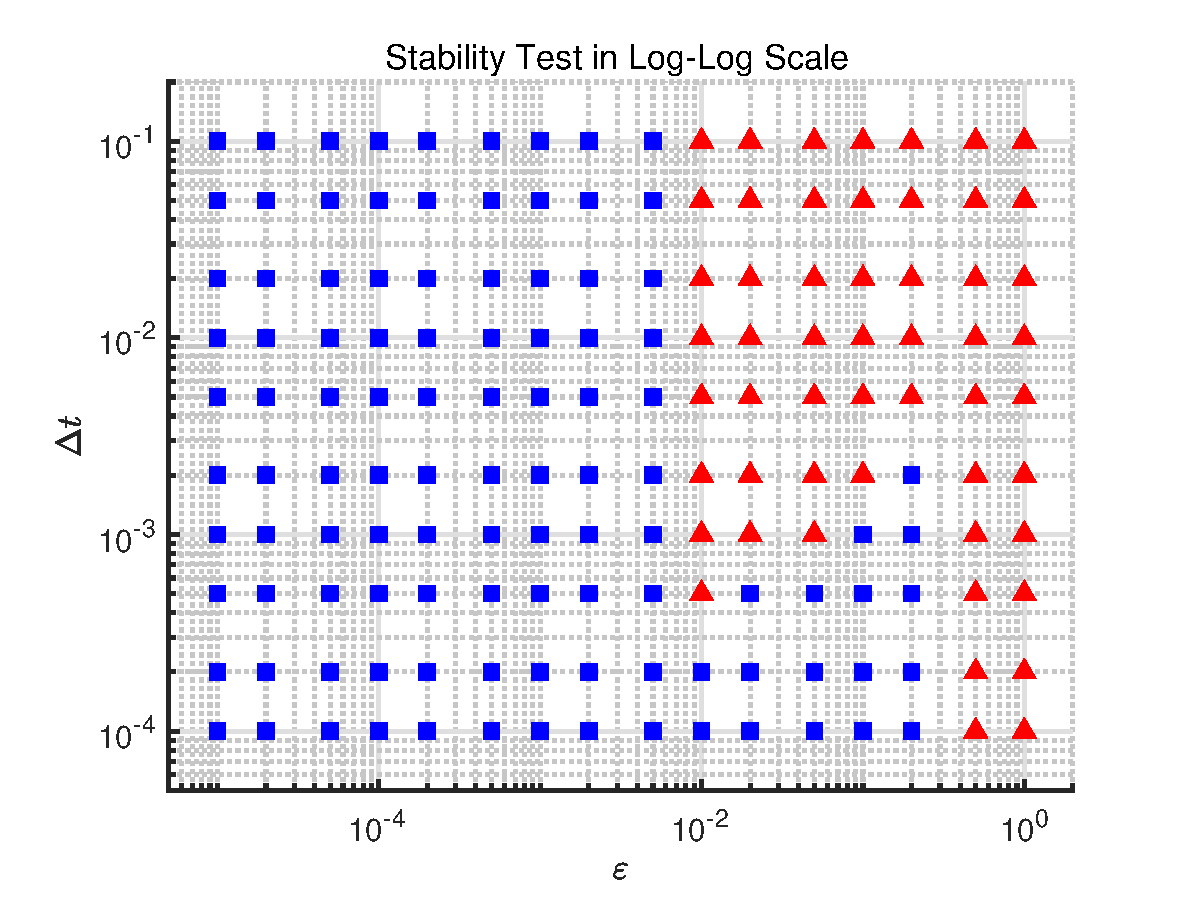
\includegraphics[scale = 0.3]{stab_test.eps}
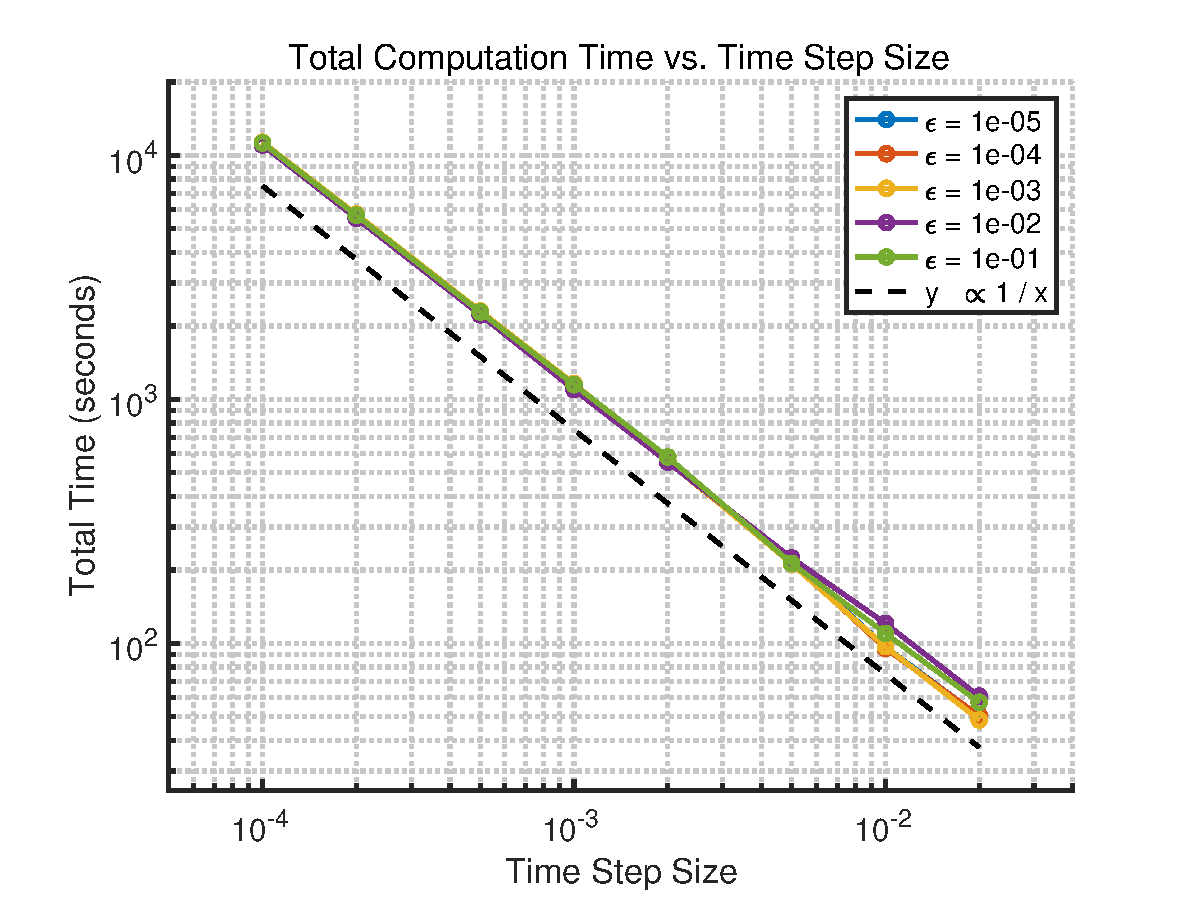
\includegraphics[scale = 0.3]{efficiency_test.eps}
}
\caption{{\color{blue}Stability and efficiency of the AP scheme for the kinetic model. The left panel evaluates stability by examining the boundedness of numerical solutions at $T=20$ for various values of $\varepsilon$ and $\Delta t$. Solutions confined within the range $[0,1]$ are marked with blue squares, whereas those extending beyond this range are denoted by red triangles. The right panel illustrates the efficiency, demonstrating that the total computational time is roughly inversely proportional to the time step size for all $\varepsilon$ values.}}
\label{fig:stab_1D}
\end{figure}


By choosing $\varepsilon = 0.2, 0.1, 0.05$ and a relatively small time step $\Delta t = 10^{-4}$, along with the initial data
\begin{align*}
	&\rho_{0_\textnormal{macro}}(x) = \rho_{0_\textnormal{kinetic}}^\varepsilon(x) = 0.5 + u(x)\ , \quad c_0(x) = c_0^\varepsilon = 0.5\ , \quad g_0^\varepsilon(x, v) = 0\ ,
\end{align*}
where $u(x)$ is a uniformly distributed random function ranging in $(-0.1, 0.1)$,
we compute the solution until $t=40$. 
In Figure \ref{fig:density_eps_A_20} we start with a comparison between $\rho_\textnormal{kinetic}^{\varepsilon}$, for different values of $\varepsilon$ {($\e = 0.2$, purple curves, $\e = 0.1$, yellow curves and $\e = 0.05$, red curves) and $\rho_\textnormal{macro}$ (blue curves), for different simulation times $t=5,\ 20,\ 32,\ 40$ (from upper left to bottom right panels, respectively)}. When the aggregates are forming ($t=5$) or merging together ($t=32$), the discrepancy between the kinetic and the macroscopic solutions are larger, specially for large values of $\e$ (purple line). As time progresses ($t=40$) this difference becomes smaller and we observe a very good agreement between the solutions of the kinetic and the macroscopic models for small values of the scaling parameter $\e$.

\begin{figure}[tbhp]
\centerline{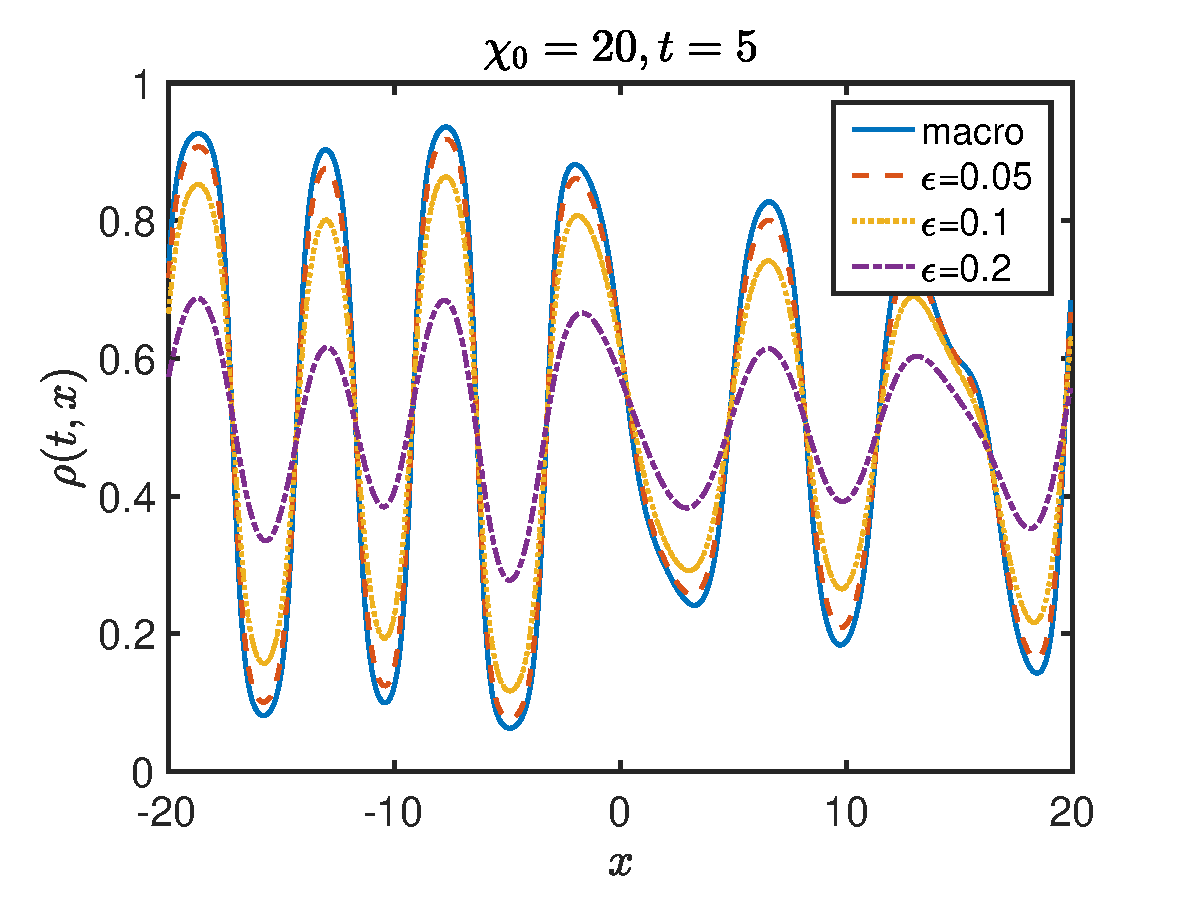
\includegraphics[scale = 0.3]{check_A_20_T_5.eps}
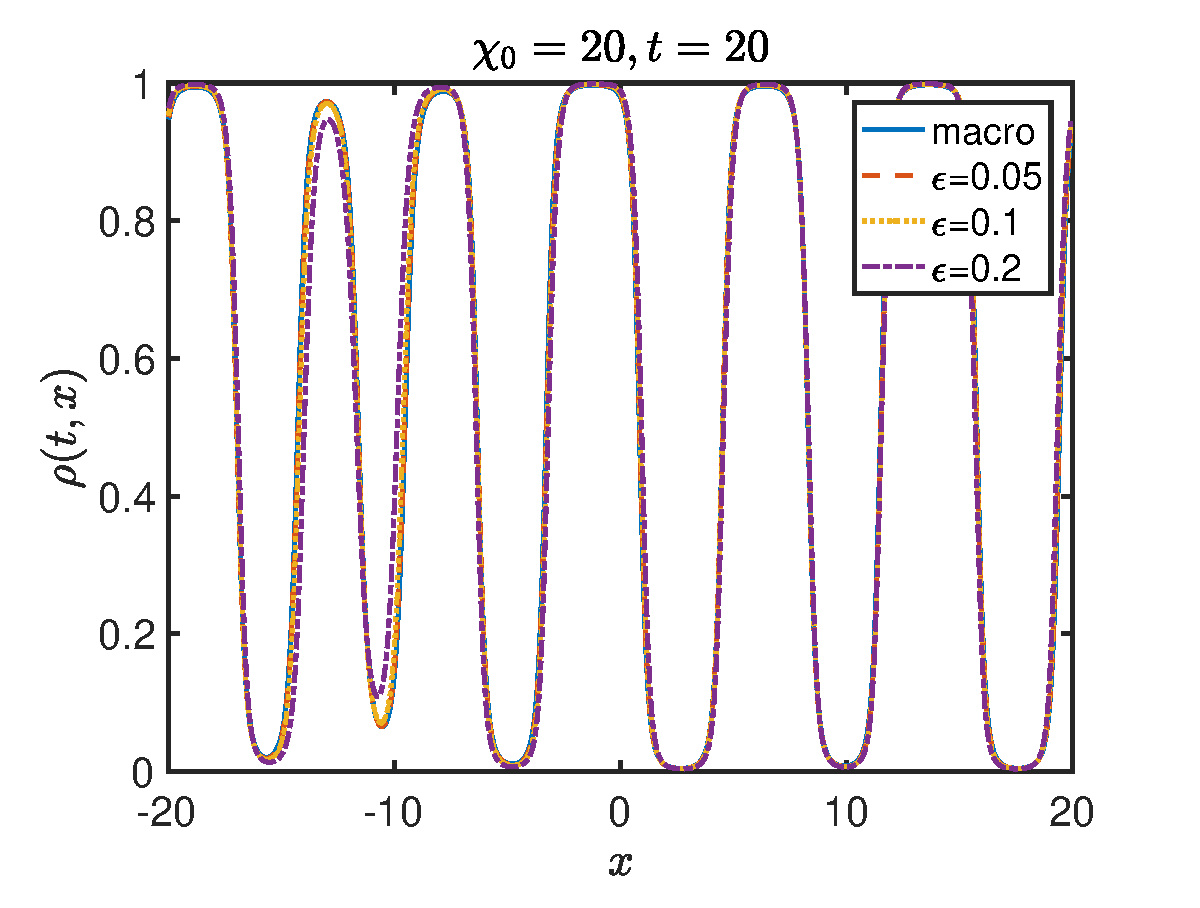
\includegraphics[scale = 0.3]{check_A_20_T_20.eps}
}
\centerline{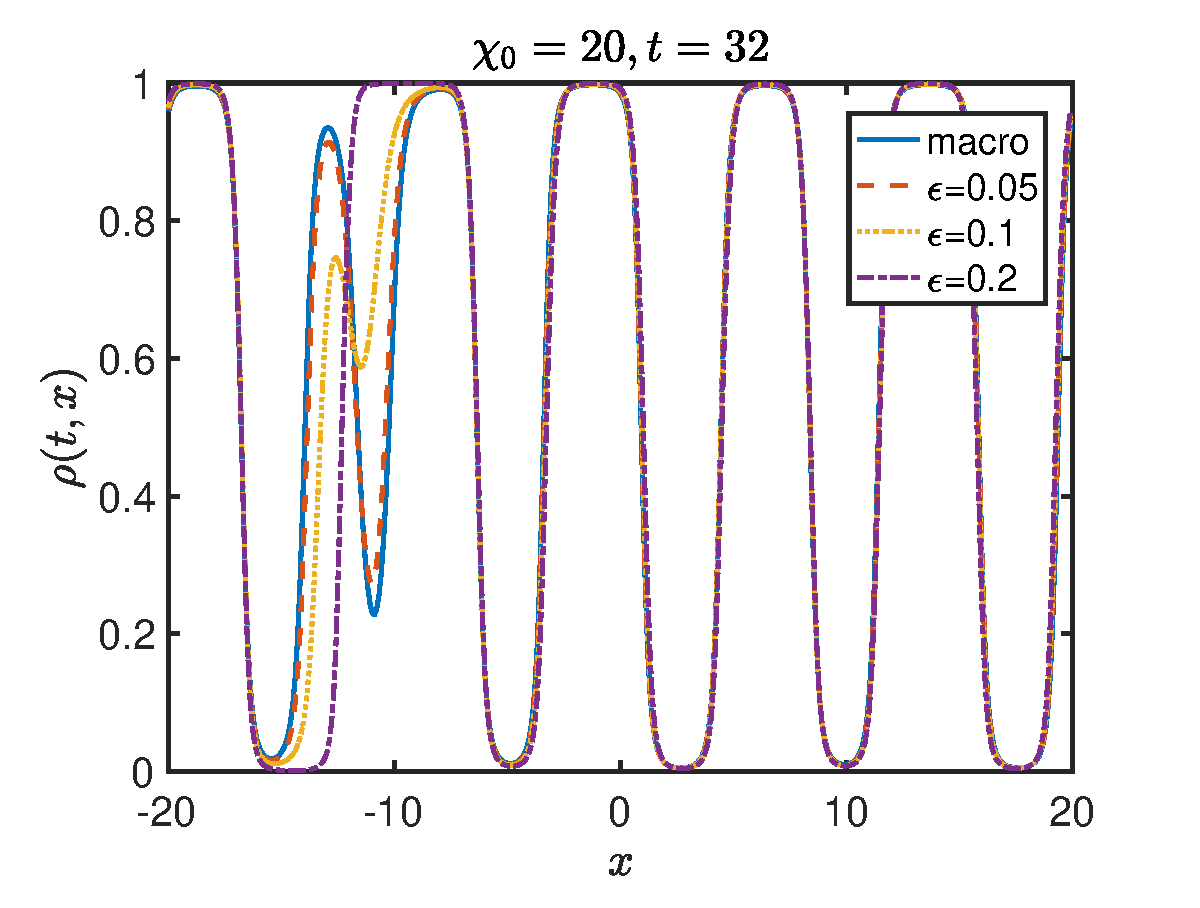
\includegraphics[scale = 0.3]{check_A_20_T_32.eps}
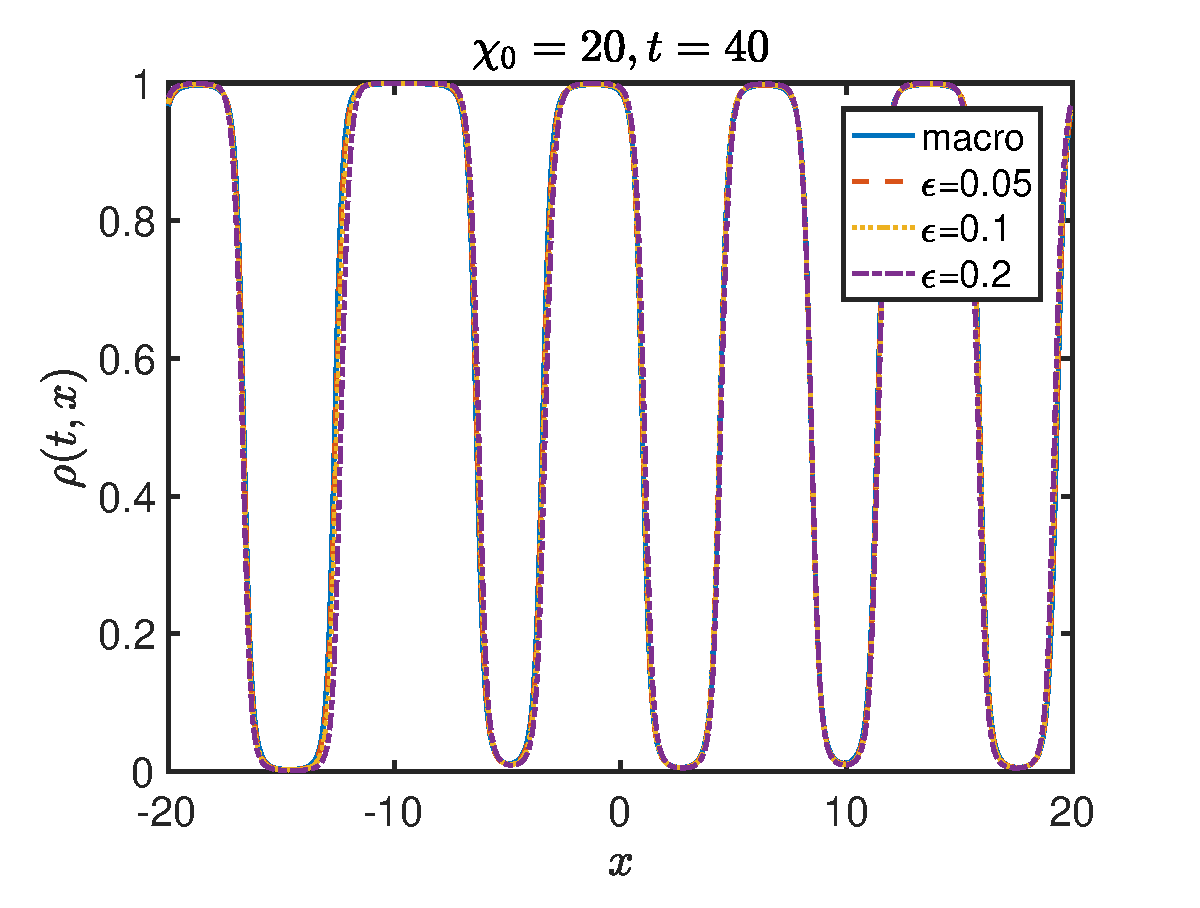
\includegraphics[scale = 0.3]{check_A_20_T_40.eps}
}
\caption{Comparison of $\rho_\textnormal{macro}$ and $\rho_\textnormal{kinetic}^{\varepsilon}$ for $\chi_0=20$,  and different values of $\e$.}
\label{fig:density_eps_A_20}
\end{figure}


{In Figure \ref{fig:plot_energy_w_sol} we show the evolution of the energy quantities $\mathcal{E}(t)$ given by \eqref{def:energy} (blue curve) and $\mathcal{E}_\varepsilon(t)$ as functions of time, for different values of $\e$: $\varepsilon=0.2$ (purple curve), $\e = 0.1$ (yellow curve) and $\e = 0.05$ (red curve), up to $t=50$. This figure shows that the energies of the kinetic and macroscopic models are in very good agreement}. \textcolor{blue}{Consistent with the analysis of Section \ref{subsec:energy}, we recover that the energy is decreasing in time for the macroscopic model. It is noteworthy that the energy defined by \eqref{def:energy} also decreases along the solutions of the kinetic model for $\epsilon>0$. These numerical results indicate that the kinetic model may possess an energy dissipation structure, the formal proof of which is left for future work.} The inset figures show the evolution in time of the macroscopic density (continuous blue line) and the kinetic density for different values of $\e$ (lines with the same style as for the energy). It is clear from these figures that the larger discrepancies between the kinetic and macro energies are indeed related with changes in the density profiles, for example when two aggregates merge together {(see the inset plots at $t=5$ and $t=32$)}. {Even in this critical case of aggregation formation we observe that the kinetic solution for $\e=0.05$ agrees with the macroscopic solution.}

A similar behaviour is observed in Figure \ref{fig:plot_energy_time} (left) where we plot the {relative} $L_2$-error between the kinetic and the macroscopic solutions {as a function of time} and for different values of $\e$ {($\e = 0.2$, black curve, $\e = 0.1$, blue curve and $\e = 0.05$, red curve)}. In agreement with the behaviour observed in Figure \ref{fig:plot_energy_w_sol} this error is {larger} at times $t=5$ and $t=32$, approximately, which corresponds {to times where aggregates are merging}.


In Figure \ref{fig:plot_energy_time} (right) we {show} the rate of convergence of the {relative} $L_2$-error between the kinetic, $\rho_\textnormal{kinetic}^\e$, and macroscopic, $\rho_\textnormal{macro}$, solutions for different values of $\e$, at different times. {We observe that the error between both solutions decreases as $\e$ decreases, and the convergence order is around 1.5 in {$\ell^2$} norm. Altogether, these first results suggest that the macroscopic and kinetic models are in good agreement for small values of $\e$, and that the kinetic model converges towards the macroscopic model as $\e \rightarrow 0$ in the 1D case. \textcolor{blue}{In Figure \ref{fig:plot_energy_time} (left) we see formations of aggregates at $t=5$ and around $t=32$, in agreement with Figure \ref{fig:plot_energy_w_sol}. For the different values of $\varepsilon$ we observe that the formation of the aggregate at $t=32$ occurs at different times, i.e., the kinetic model seems to converge faster to the ``aggregated-state'' compared to the macroscopic dynamics. These changes in speed could be a result of the diffusion scaling, where the macroscopic model is obtained in a regime where there are many velocity jumps but small net displacements in one order of time (see \cite{Alt1980, patlak1953random,Hillen2009,painter2002volume} for thorough interpretations of the diffusion scaling).}  In the next section, we take a step further and analyze the evolution of the pattern sizes in time as function of the chemotactic sensitivity  $\chi_0$.

\begin{figure}[tbhp]
\centerline{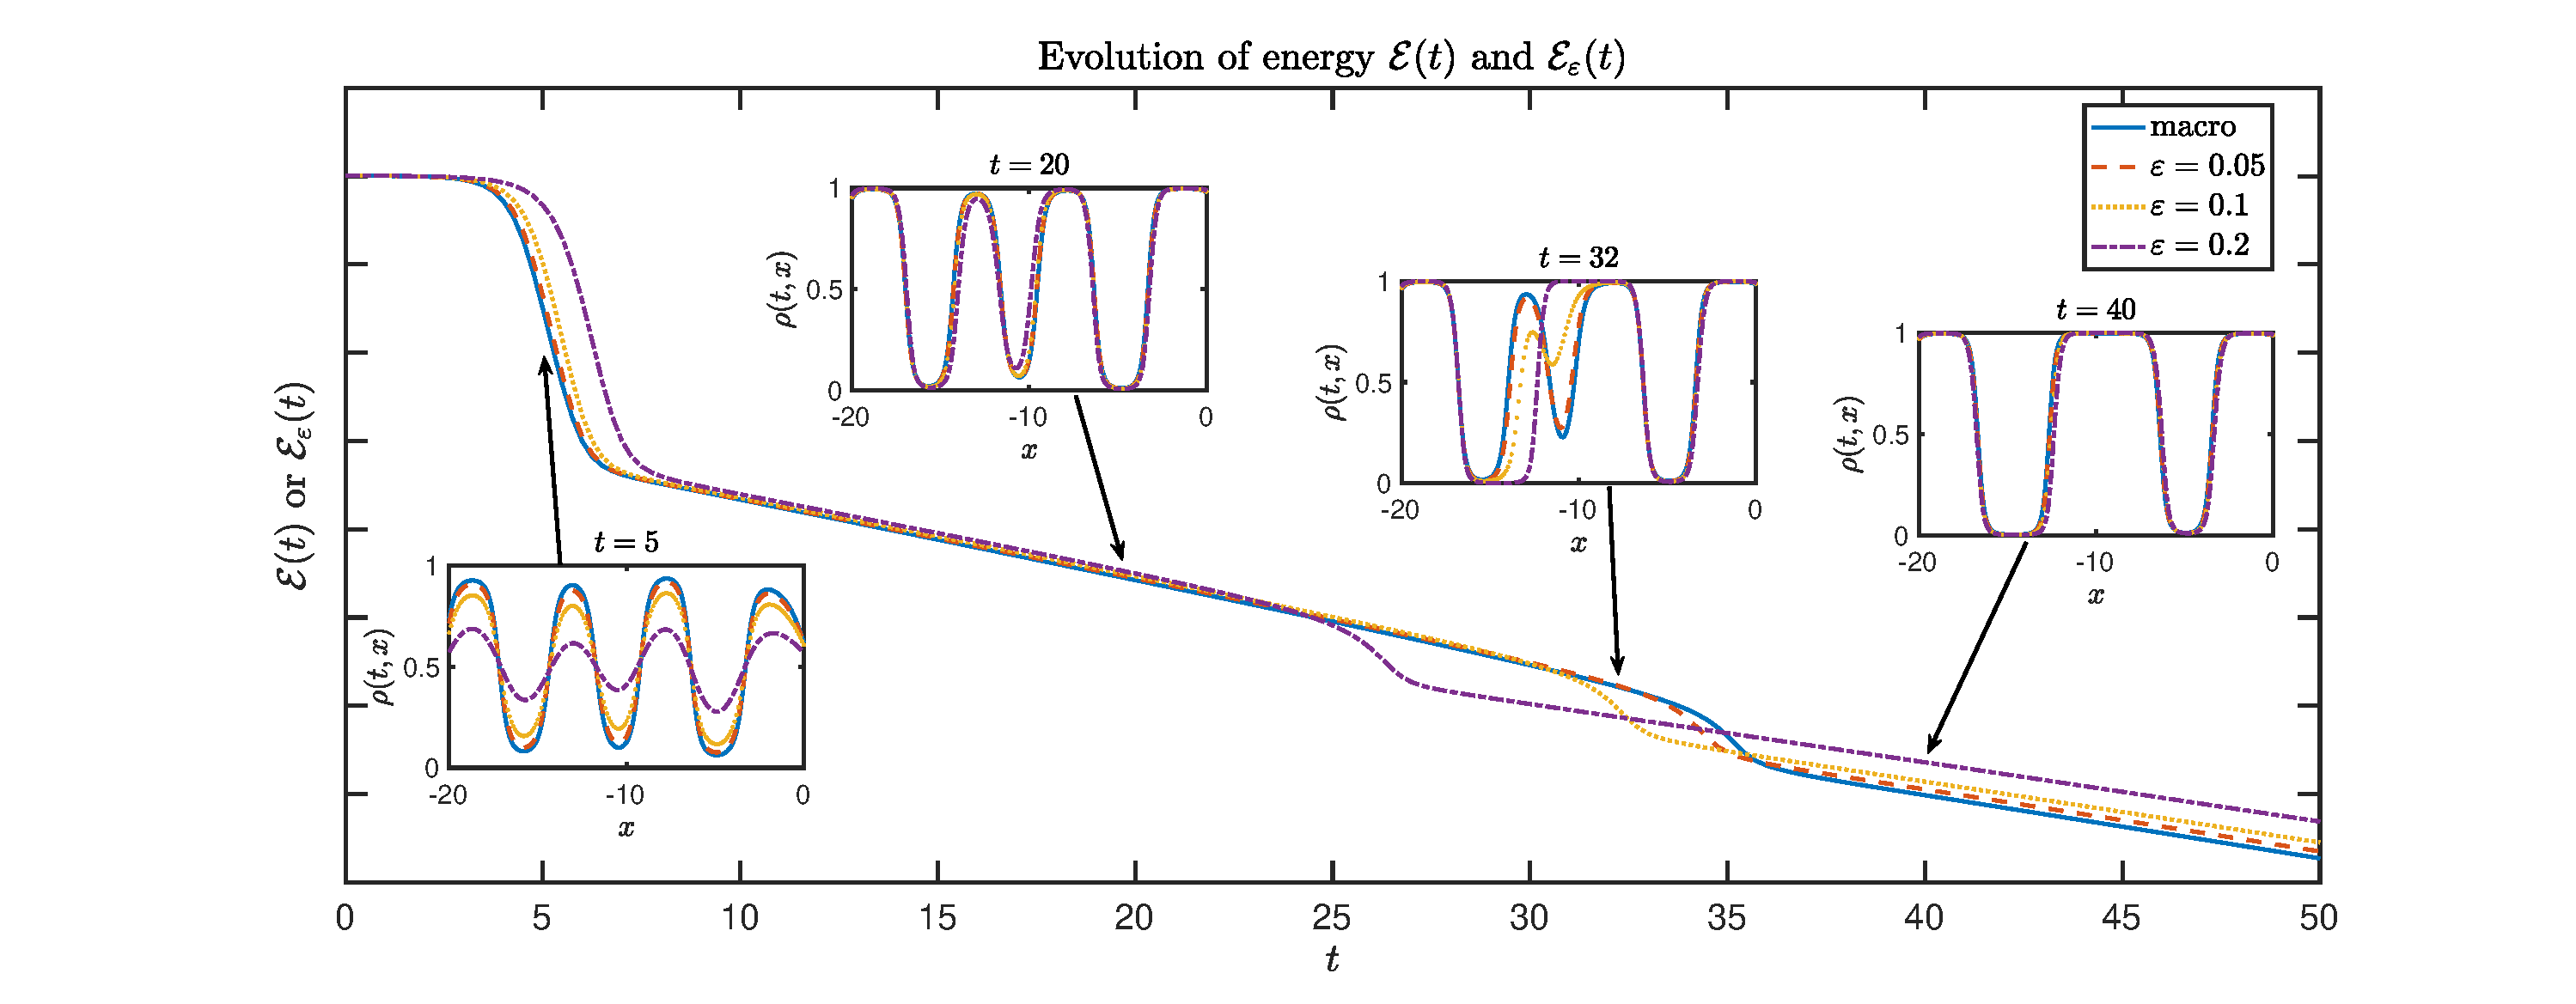
\includegraphics[scale = 0.3]{energy_A_20_T_50_w_sol.eps}
}
\caption{Evolution of $\mathcal{E}(t)$ and $\mathcal{E}_\e(t)$ along with the comparison between the kinetic solutions $\rho_\textnormal{kinetic}^\varepsilon$ and the macroscopic solutions $\rho_\textnormal{macro}(t,x)$ at $t=5,\ 20,\ 32,\ 40$ for $\chi_0=20$.}
\label{fig:plot_energy_w_sol}
\end{figure}

\begin{figure}[tbhp]
\centerline{
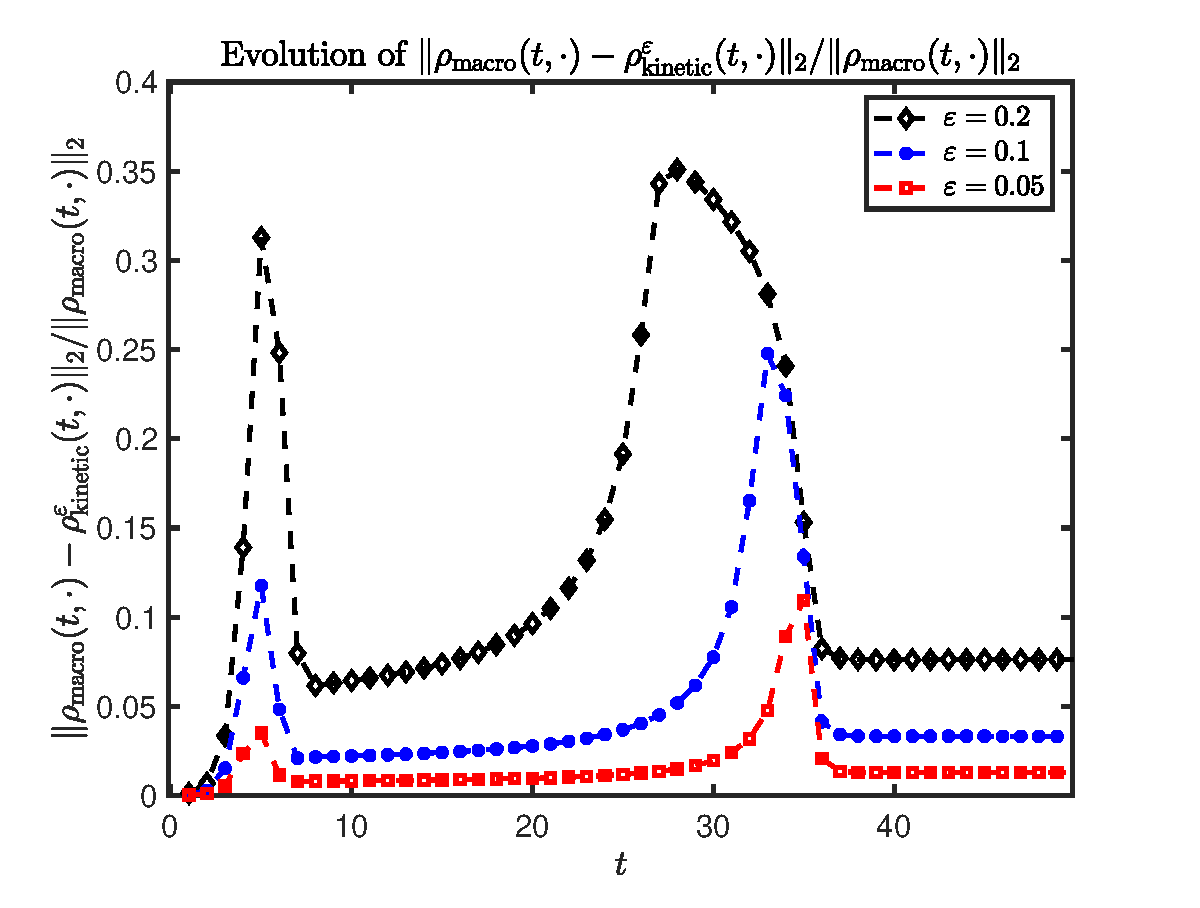
\includegraphics[scale = 0.3]{l2_relative_err_evolution_A_20_T_50.eps}
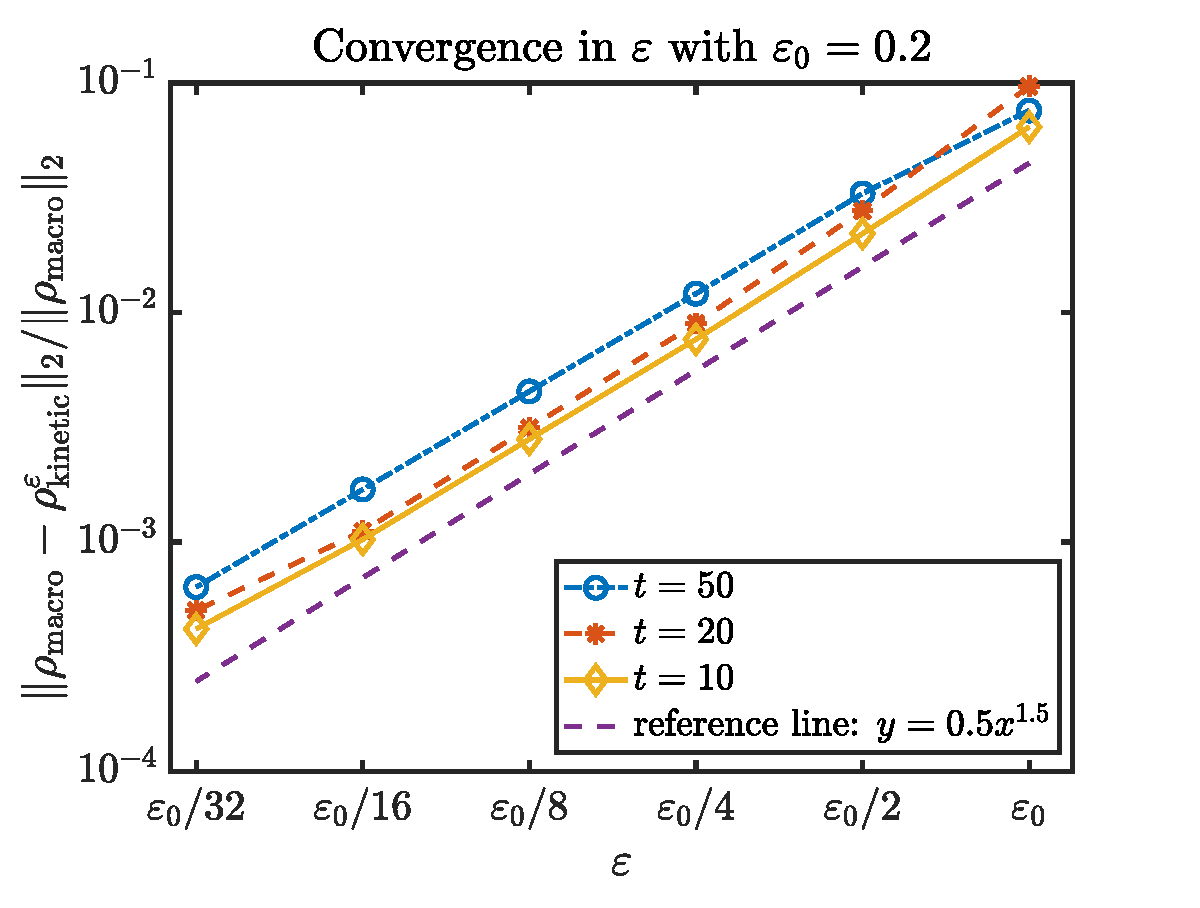
\includegraphics[scale = 0.3]{check_l2_relative_err_A_20.eps}
}
\caption{Left: Evolution of the {relative} $L_2$-error $\frac{\|\rho_{\rm{macro}}(t, \cdot) - \rho_{\rm{kinetic}}(t,\cdot)\|_2}{\|\rho_{\rm{macro}}(t, \cdot)\|}$ over time with $\chi_0=20$. Right: Convergence of the relative $L_2$-error in $\e$  at $t=10,\  20, \ 50$. The numerical setting is the same as in Figure \ref{fig:density_eps_A_20}.}
\label{fig:plot_energy_time}
\end{figure}


\subsection{Pattern formation from a perturbed 1D initial data}
With a strong chemotaxis effect, cells will aggregate to form patterns in regions where the chemoattractant is highly concentrated. 
For the volume-exclusion Keller-Segel model \eqref{eq:macro_proliferation}, the relation between the aggregate size from { an initial data perturbed from some homogeneous steady state} and the strength of chemotaxis effect $\chi_0$ {was proven in \cite{almeida2020treatment} via linear stability analysis. }
{

}
In this section, we numerically verify this relation for both the kinetic \eqref{eq:kinetic_approx} and the macroscopic model \eqref{eq:macro_proliferation}. 
{Again, we only consider here the 1D case with periodic boundary conditions in space. 
More specifically, we consider the domain $(x,v)\in (-20,20)^2$ with a uniform mesh {$\dx = 0.1,\  \Delta v =  0.2$}. We choose the time step $\Delta t = 10^{-3}$ and starting from a randomly perturbed initial data
\begin{equation*}
    \rho_{0_\textnormal{macro}}(t,x) = \rho_{0_\textnormal{kinetic}}^{\varepsilon}(t,x) = 0.5 + u(x)\ ,
\end{equation*}
we let the simulation run until $t=20$. 
To avoid effects due to the randomness of the initial data, we will compute the pattern size for 10 solutions, each evolved from some random initial data, and simply average. }

To numerically compute the pattern sizes, we consider the Fourier transform of the density function $\rho(t,x)$ (macro and kinetic) and extract the frequency that corresponds to the maximal Fourier mode. 
Specifically, we consider
\begin{equation*}
    k_{\rm max} = \rm{argmax}_{\lambda} (|\hat{\rho}(\lambda)|)\ , 
\end{equation*}
where $\hat{\rho}(\lambda) = \mathcal{F}(\rho)(t,x)$ is the Fourier transform of the density function $\rho(t,x)$. 
Then, $1/k_{\rm max}$ can be used to describe the pattern size. 
{ With the numerical experimental settings in Section \ref{subsec:energy_dissipation}, here we compare the numerical results with the following formula, which was proposed in \cite{almeida2020treatment}, 
\begin{equation*}
k_{\rm max}^{\rm analytical} = {\rm argmax}_{k} \left\{- \frac{k^4 - \left(\frac{\chi_0}{4}-1.1\right)k^2 +0.1}{k^2+1} \right\} = \sqrt{\frac{\sqrt{\chi_0}}{2} - 1}.
\end{equation*}
} 

\begin{figure}[tbhp]
\centerline{
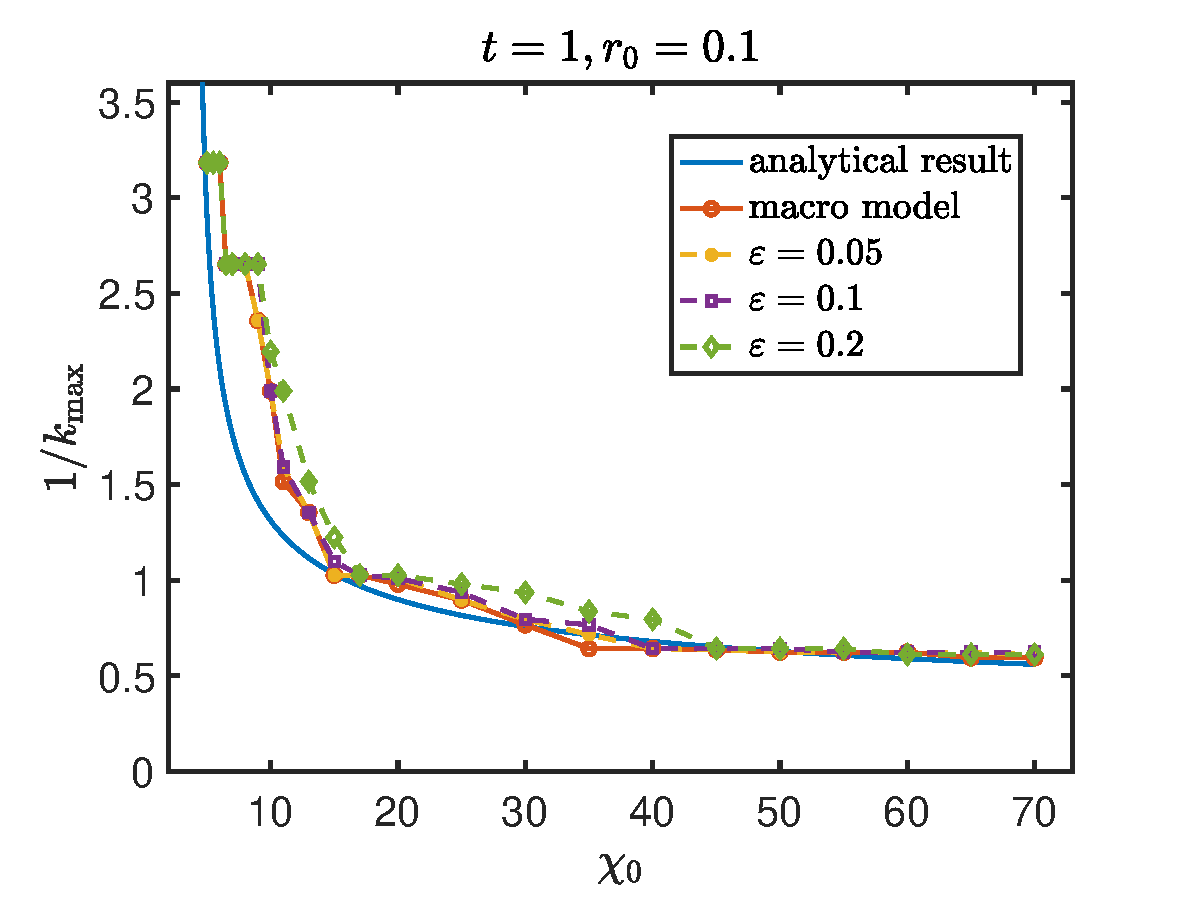
\includegraphics[scale = 0.3]{compare_k_T_1.eps}
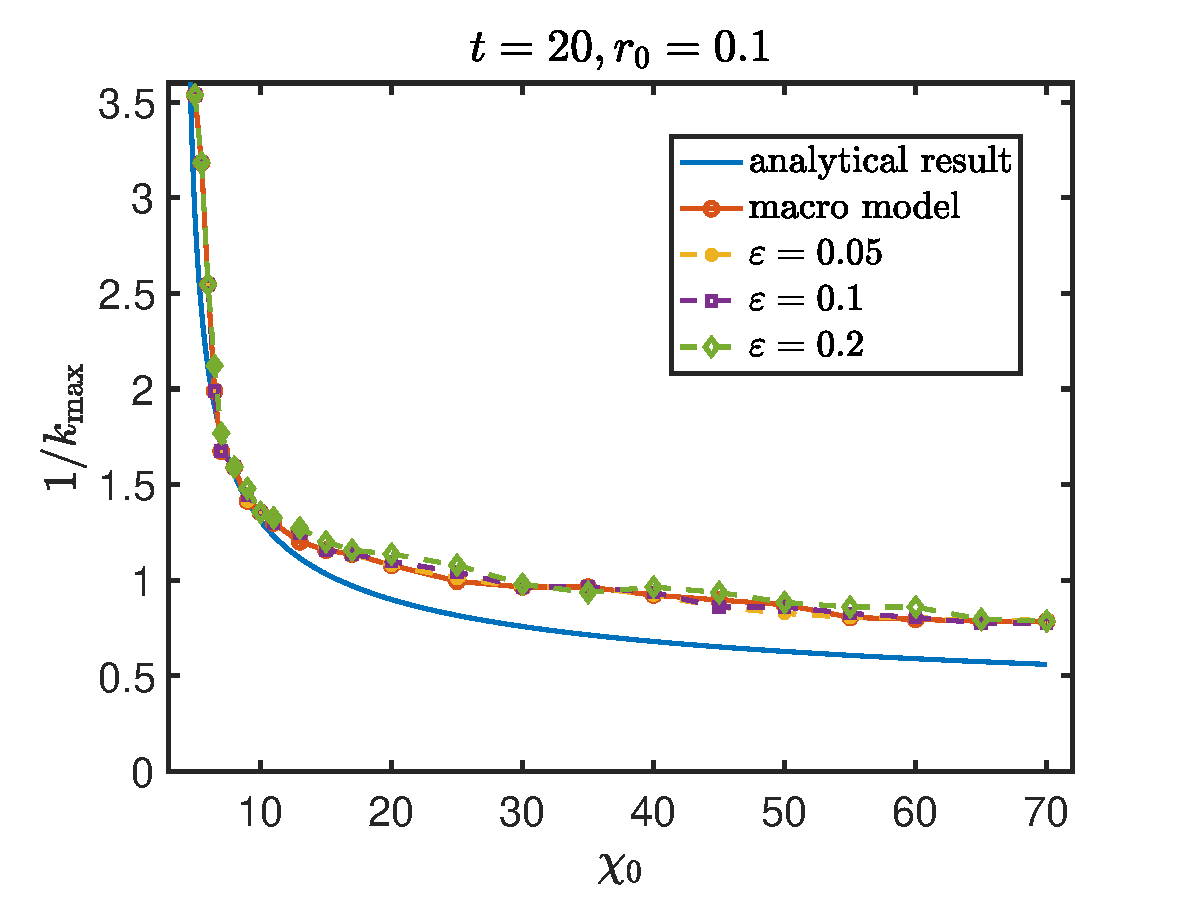
\includegraphics[scale = 0.3]{compare_k_T_20.eps}
}
\caption{Comparison of $\frac{1}{k_{\textnormal{max}}}$ between the analytical, the numerical results of the macro and the kinetic model. The numerical result is computed by averaging 10 solutions, each evolved from a random initial data around $0.5$.}
\label{fig:k2_inv_compare}
\end{figure}


In Figure \ref{fig:k2_inv_compare} we show the overall pattern sizes $1/k_{\rm max}$ as a function of the chemotaxis sensitivity $\chi_0$ 
at times $t=1$ (left panel) and $t=20$ (right panel). 
For each time, we plot the analytical prediction of $\frac{1}{k_{\max}}$ (blue line, see Ref.~\cite{almeida2020treatment}), the numerical result for the macroscopic model (red line) and the results for the kinetic model with various values of $\e$ ($\e = 0.05$ in yellow, $\e = 0.1$ in purple and $\e = 0.2$ in green lines). 
As one can observe, we obtain a very good agreement between the predicted pattern sizes and the ones computed numerically for both the macroscopic and kinetic models. 
{ With a strong chemotaxis sensitivity, cells aggregate more quickly to form patterns and, therefore, we can observe the agreement within a short time. 
It will take longer time to observe the agreement for cases with a relatively weak chemotaxis sensitivity.
It explains why in Figure \ref{fig:k2_inv_compare} the good agreement between the predicted pattern sizes and the numerical ones can be observed at $t=1$ when $\chi_0$ is large while the same phenomenon for small $\chi_0$ can only be observed when $t=20$. 
}
As predicted by the stability analysis performed in \cite{almeida2020treatment}, the pattern sizes decrease as the chemotactic sensitivity $\chi_0$ increases, and we recover the critical value $\chi_0^* \approx 6.9$ below which there are no patterns, i.e for which the perturbations are damped and the solution comes back to a homogeneous distribution. 


\subsection{2D numerical examples}
The numerical schemes for both the kinetic model \eqref{eq:scheme} and the macroscopic model \eqref{scheme:limit} can be generalized to multi-dimensional problems, where the tensor-product grid is adopted {(see Section \ref{sec:appendix-FD-2D} for a detailed description of the 2D numerical scheme for the kinetic model)}. 

In this section we perform 2D simulations for both  {{the kinetic model \eqref{eq:kinetic_approx}}} and  {{the volume-exclusion Keller-Segel model \eqref{eq:macro_proliferation}}}. 
We consider the computation domain $\Omega_\mathbf{x} = \{\mathbf{x} = (x_1,x_2)\in\mathbb{R}^2: -20\le x_1, x_2 \le 20\}$ with a uniform mesh $\Delta x_1 = \Delta x_2 = 0.1$ and periodic boundary conditions.  
For the kinetic model \eqref{eq:kinetic_approx}, we need to further define the domain of the velocity $\Omega_\mathbf{v} = \{\mathbf{v} = (v_1,v_2)\in\mathbb{R}^2: -10\le v_1, v_2 \le 10\}$ with a uniform mesh $\Delta v_1 = \Delta v_2 = 0.2$ and zero boundary conditions. 
We choose $r_0=0.1$, $\rho_{\rm max} = 0.5$, $\bar{\rho} = 1$ and 
\begin{equation*}
    \psi_0(\mathbf{v}) = \frac{1}{2\pi} e^{-\frac{|\mathbf{v}|^2}{2}}, \quad \psi_1(\mathbf{v}\ , \nabla_\mathbf{x} c) = \frac{\mathbf{v}}{2\pi} e^{-\frac{|\mathbf{v}|^2}{2}}\cdot \nabla_\mathbf{x} c\ .
\end{equation*}
As in the 1D case, we can check that the choices of $\psi_0(\mathbf{v})$ and $\psi_1(\mathbf{v})$ satisfy the Hypotheses \ref{hypo1} and \ref{hypo2}.


We fix $\Delta t = 10^{-3}$ and choose the initial data to be
\begin{align*}
	&\rho_{0_\textnormal{macro}}(\mathbf{x}) =  \rho_{0_\textnormal{kinetic}}^\varepsilon(\mathbf{x}) =  \rho_0 + u(x)\ , \quad c_0(\mathbf{x}) = c_0^\varepsilon(\mathbf{x}) = 0.5\ , %\quad g_0^\varepsilon(\mathbf{x}, \mathbf{v}) = 0,
\end{align*}
where $u(x)$ is a randomly chosen uniformly distributed function ranging in $(-0.1, 0.1)$. 
In Figure \ref{fig:2D_macro} we show the numerical results at $t=5$ (first row), $t=20$ (second row) and $t=50$ (third row) for the macroscopic model with different chemotaxis sensitivities $\chi_0=6$ (first column), $\chi_0=20$ (second column) and $\chi_0=50$ (third column). As one can observe, starting from an initial data perturbed around the homogeneous value $0.5$, we obtain the formation of labyrinthic patterns for a chemotactic sensitivity $\chi_0>6$ (middle and right columns), while the solution dampens to the homogeneous state for $\chi_0=6$ (left column), in agreement with the predictions of the stability analysis performed in \cite{almeida2020treatment} and the results in Figure \ref{fig:k2_inv_compare}. Moreover, we observe that larger values of the chemotactic sensitivity $\chi_0$ {lead} to sharper layers near the boundary of the patterns (compare middle and right columns) as expected. 

{\color{blue} The convergence of the numerical patterns towards $\varepsilon\to0$ is illustrated in Fig. \ref{fig:2D_convergence_sol}. 
In this test, we choose $\varepsilon = 10^{-1}, 10^{-2}, 10^{-3}$ and consider  chemotactic sensitivities $\chi_0 = 20$ and $\chi_0 = 50$, along with two different initial densities: $\rho_0 = 0.5$ and $\rho_0 = 0.1$. 
As observed in \cite{painter2002volume}, different initial conditions lead to qualitatively different pattern types for both kinetic and macroscopic models: labyrinthine patterns for $\rho_0 = 0.5$, and spot-like patterns for $\rho_0 = 0.1$. Moreover, we note that increasing $\chi_0$ leads to smaller and sharper patterns in the kinetic model as well.}
% in the case of round patterns (last two columns Fig. \ref{fig:2D_compare}), and again that the boundary of the patterns become sharper in the case of labyrinthic patterns (compare the first two columns) also for the kinetic solution. %These results are in very good agreement with the predictions of the stability analysis, and observed for both the macroscopic model and the kinetic one with $\varepsilon = 10^{-2}$, which are in very good agreement (compare the two columns). 

In order to quantify the differences between the kinetic and macroscopic 2D models, we show in Figure \ref{fig:2D_convergence} (left) the evolution in time of the relative $L^2$-error between the macroscopic and kinetic models for different values of $\varepsilon$: $\varepsilon = 10^{-2}$ (blue curve), $\varepsilon = 10^{-4}$ (red curve), $\varepsilon = 10^{-6}$ (yellow curve), $\varepsilon = 10^{-8}$ (purple curve), and Figure \ref{fig:2D_convergence} (right) shows this relative error as function of $\varepsilon$ for different time points: $t=1$ (blue curve), $t=3$ (red curve), $t=5$ (yellow curve) and $t=10$ (purple curve). We observe that the relative error between both models decreases as $\varepsilon$ decreases, and the reference line $y = x$ (green curve) shows that the rate of convergence of the kinetic model towards the macroscopic one is roughly $\mathcal{O}(\varepsilon)$.

\begin{figure}[tbhp]
\centerline{
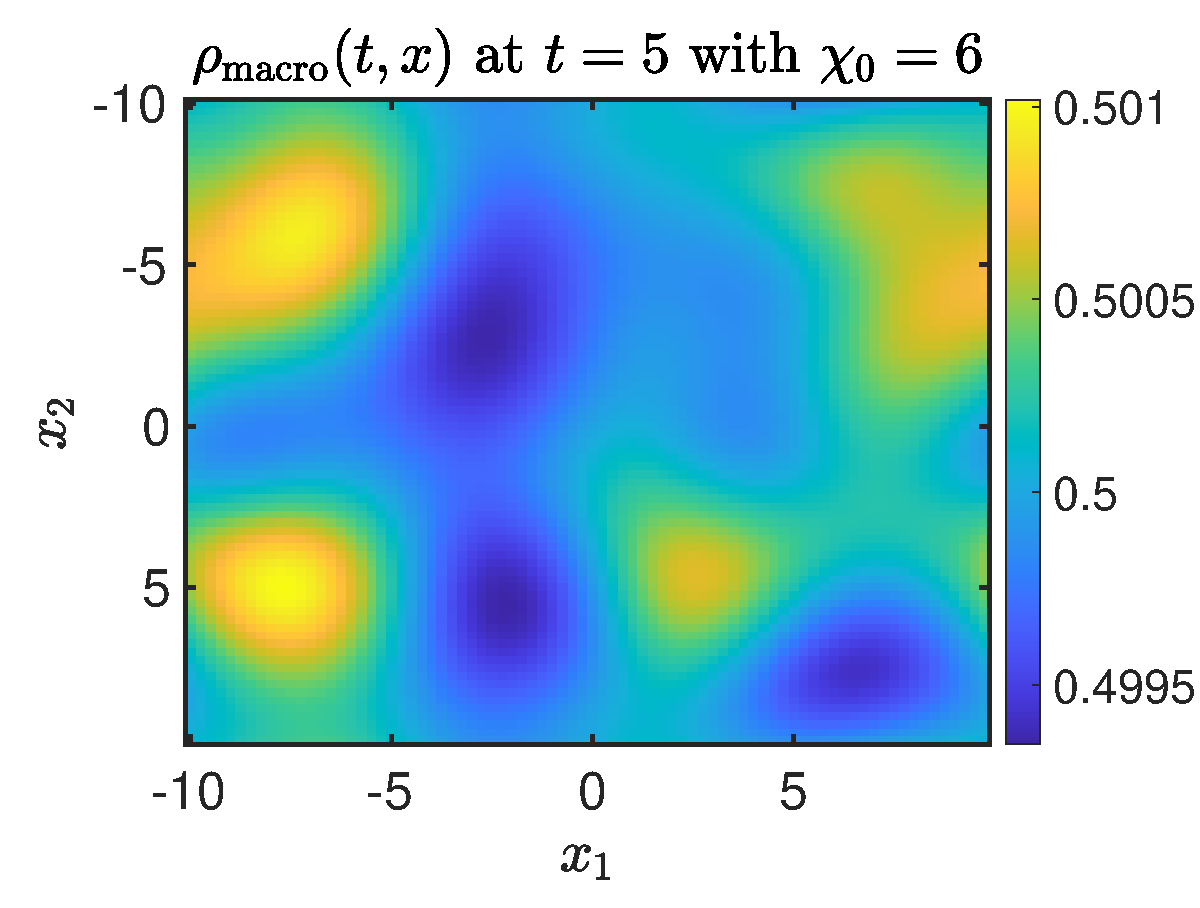
\includegraphics[scale = 0.2]{sol2D_A_6_T_5.eps}
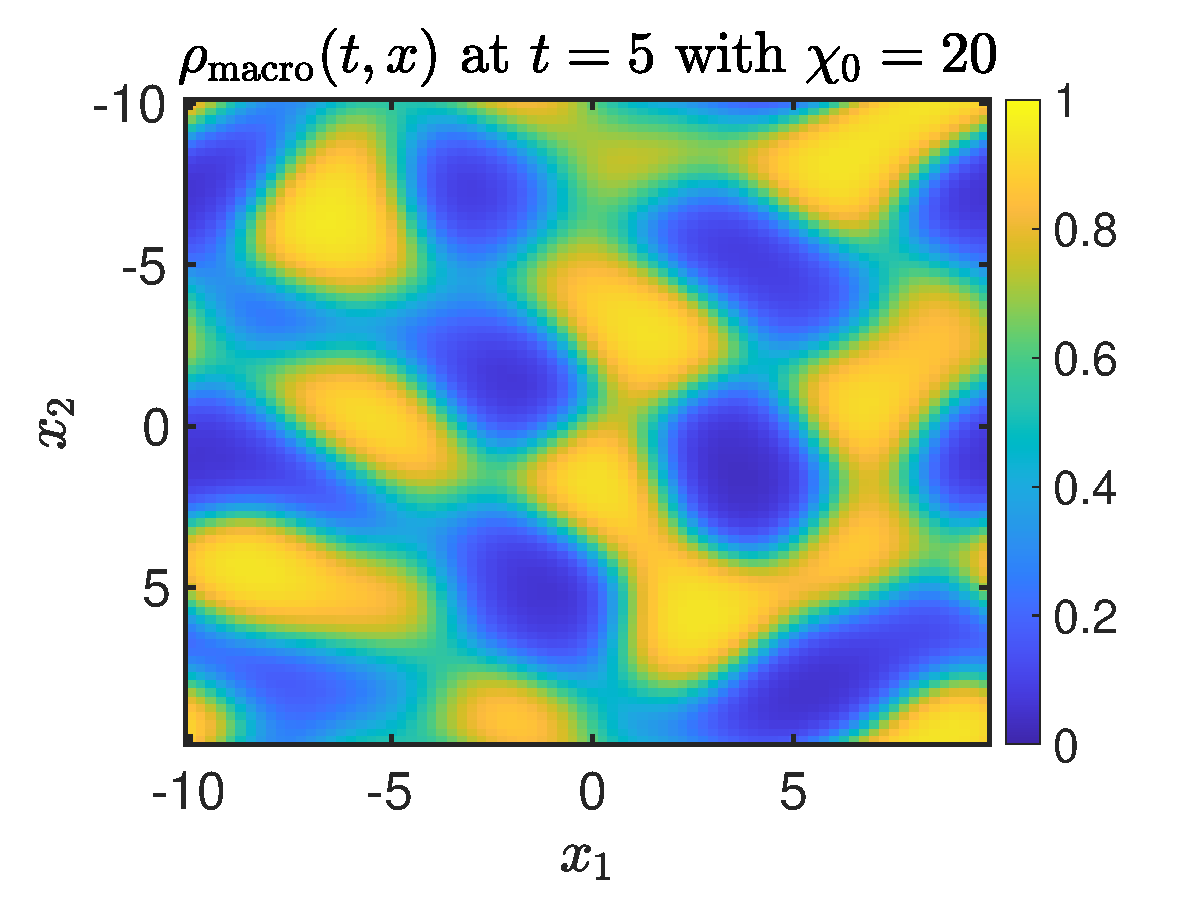
\includegraphics[scale = 0.2]{sol2D_A_20_T_5.eps}
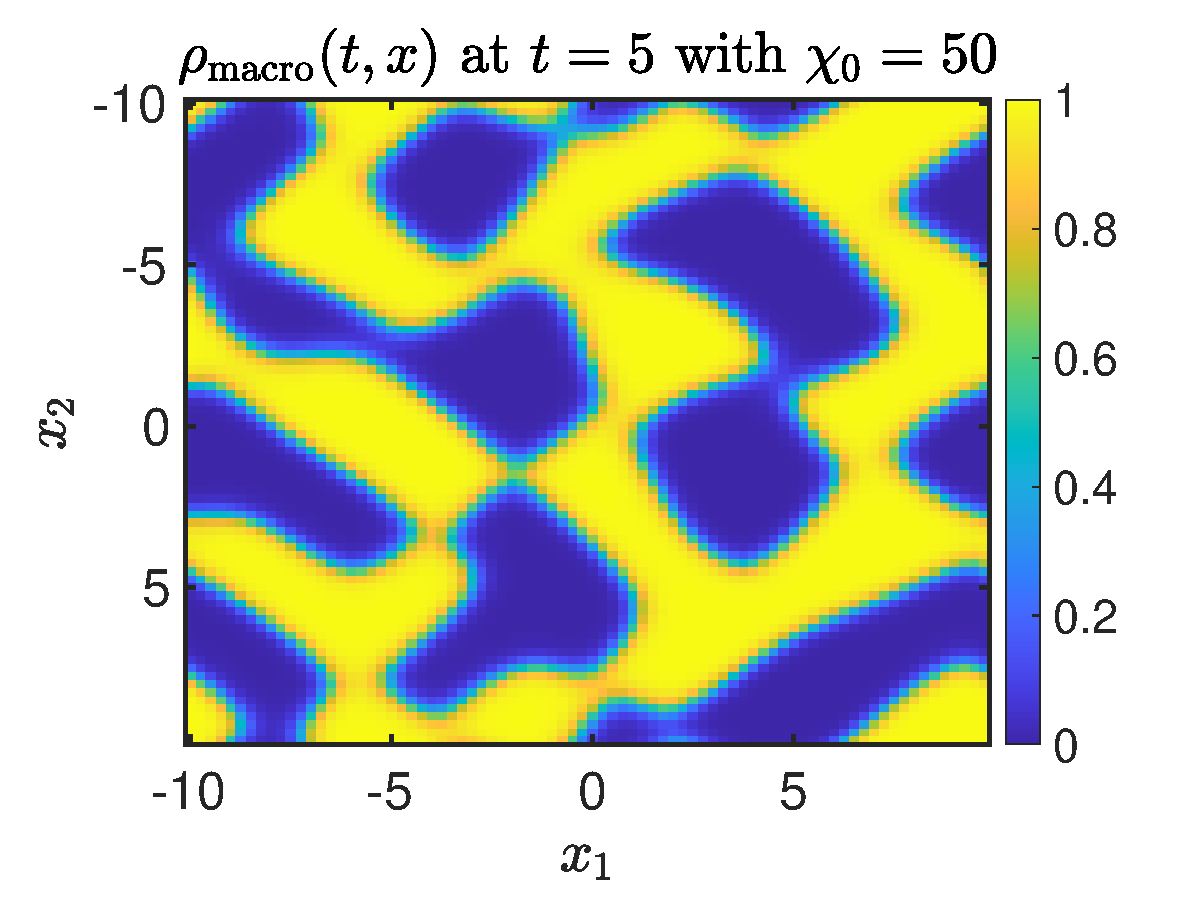
\includegraphics[scale = 0.2]{sol2D_A_50_T_5.eps}
}
\centerline{
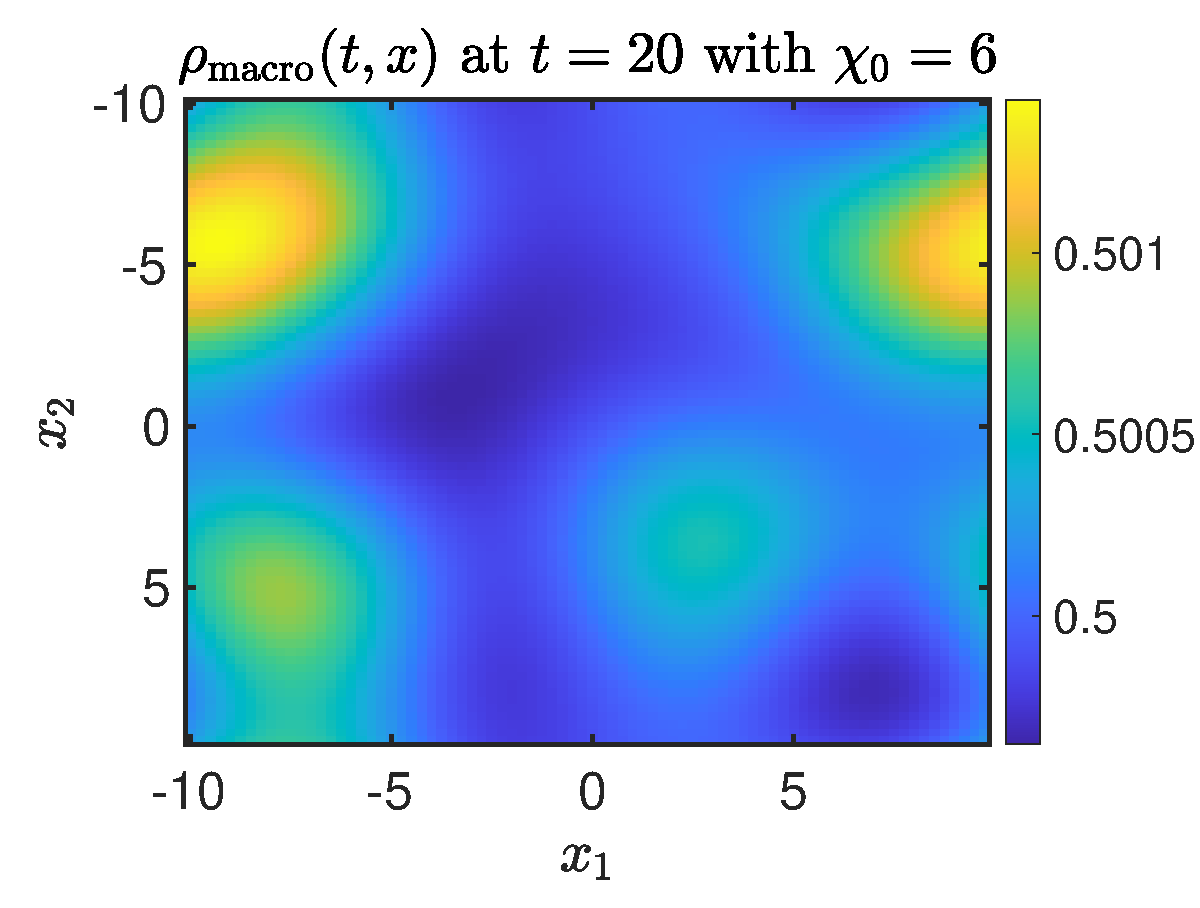
\includegraphics[scale = 0.2]{sol2D_A_6_T_20.eps}
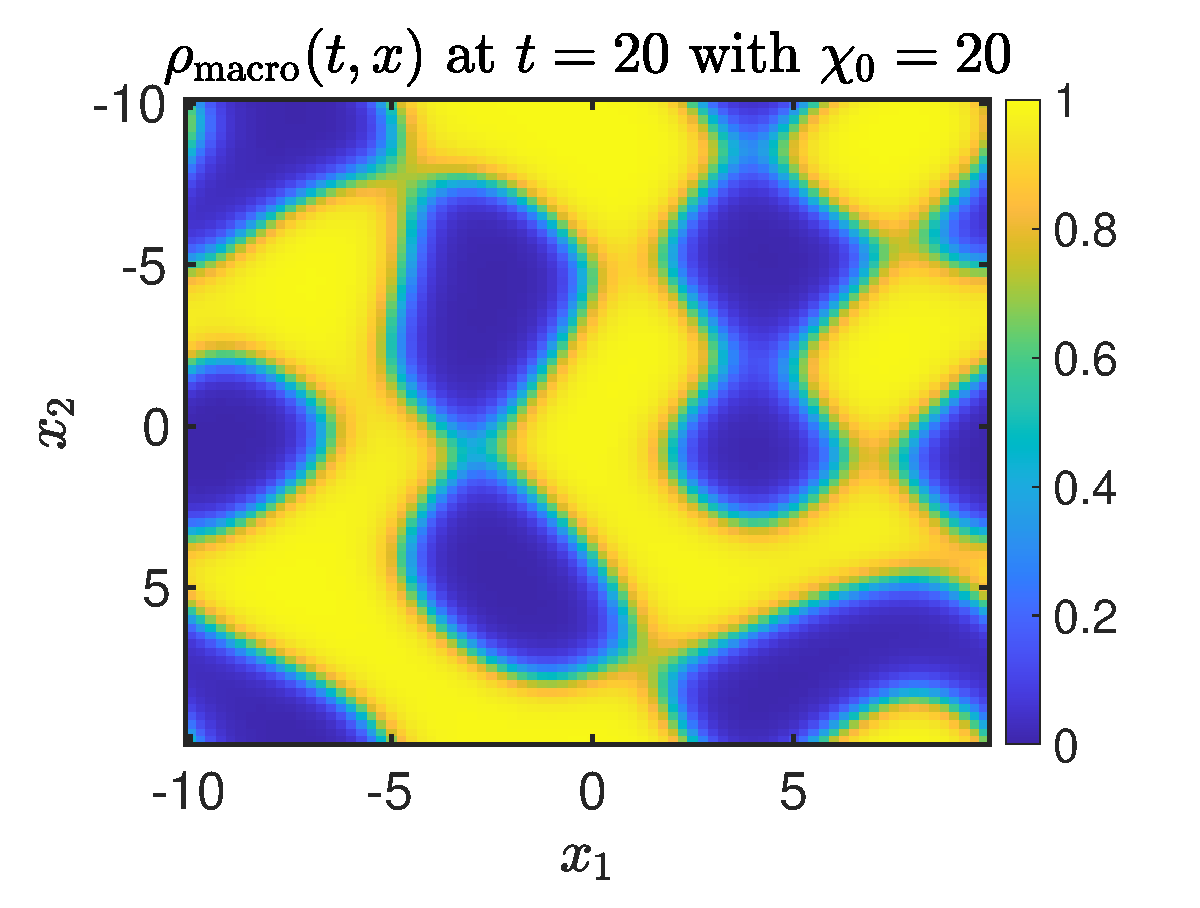
\includegraphics[scale = 0.2]{sol2D_A_20_T_20.eps}
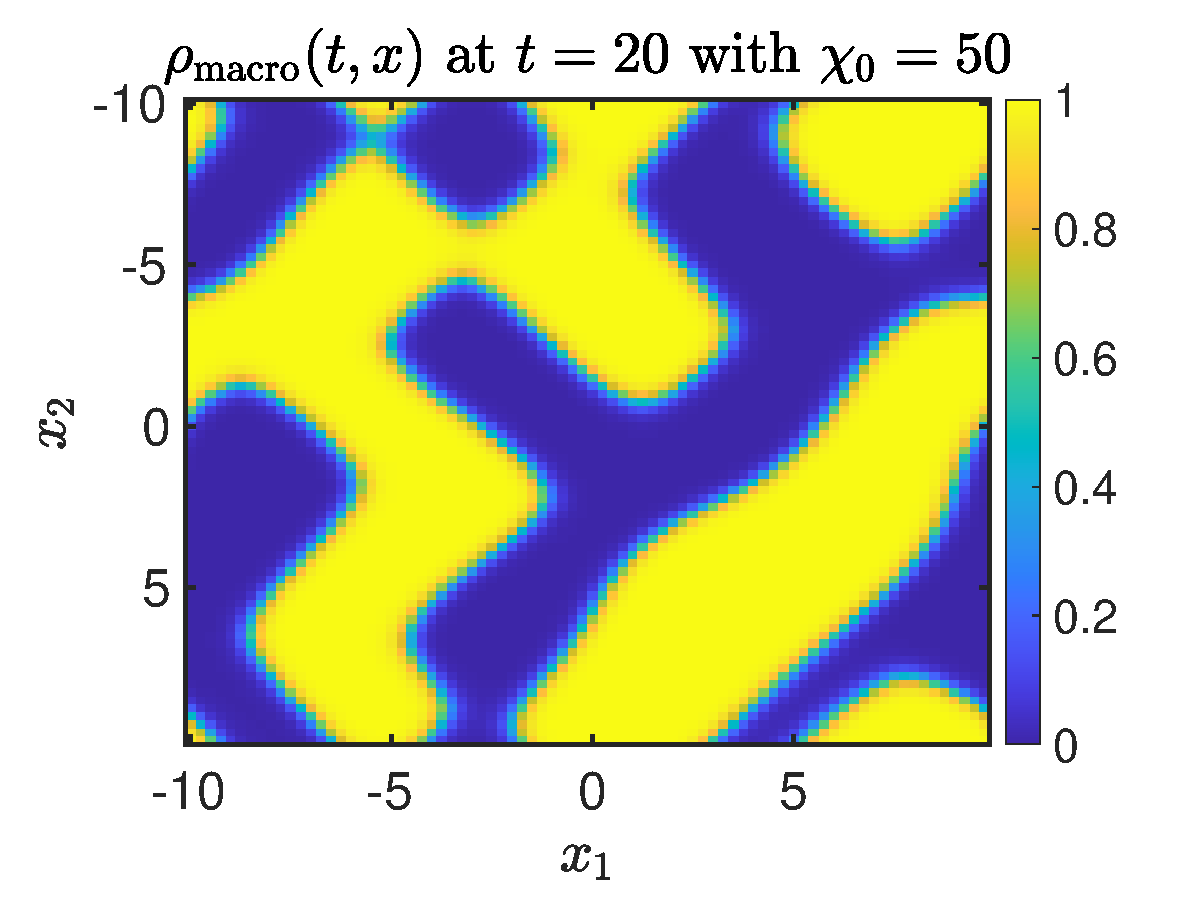
\includegraphics[scale = 0.2]{sol2D_A_50_T_20.eps}
}
\centerline{
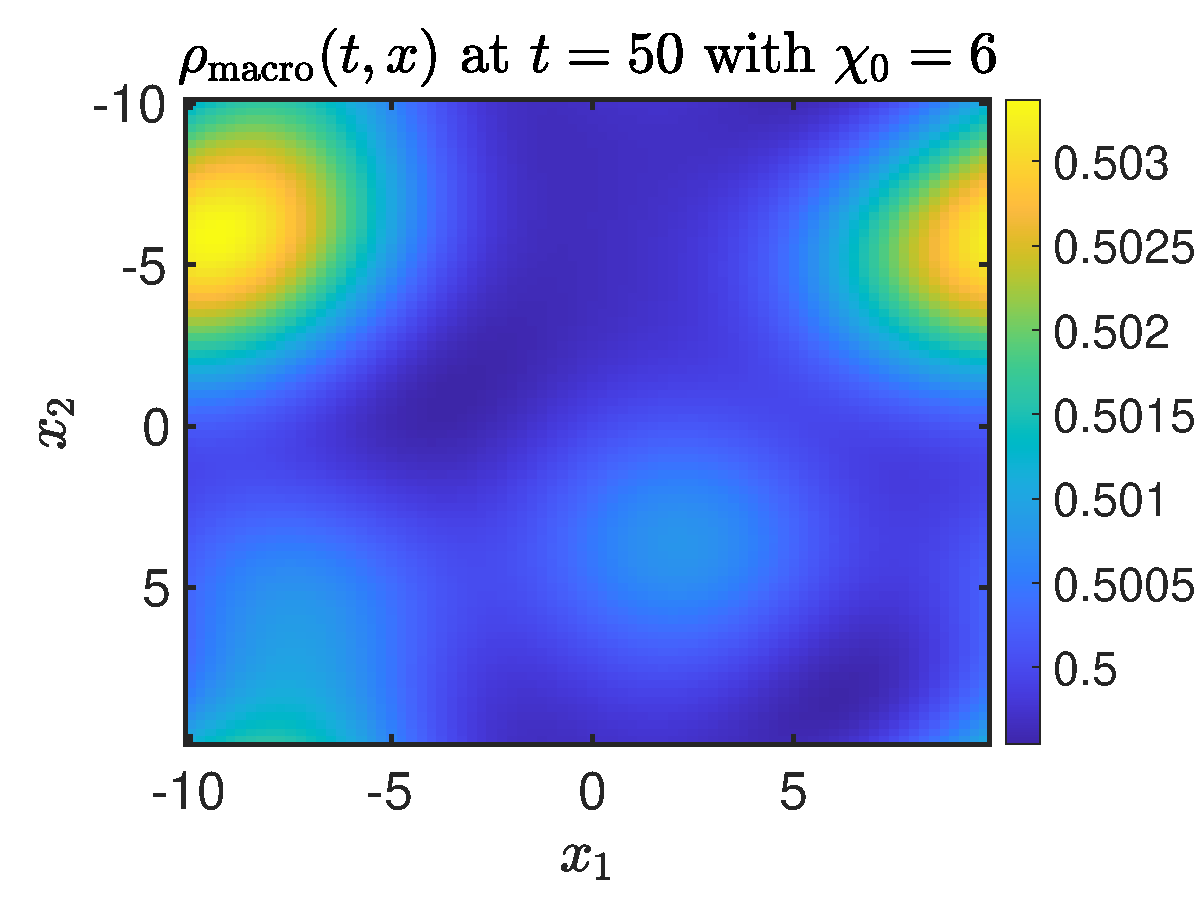
\includegraphics[scale = 0.2]{sol2D_A_6_T_50.eps}
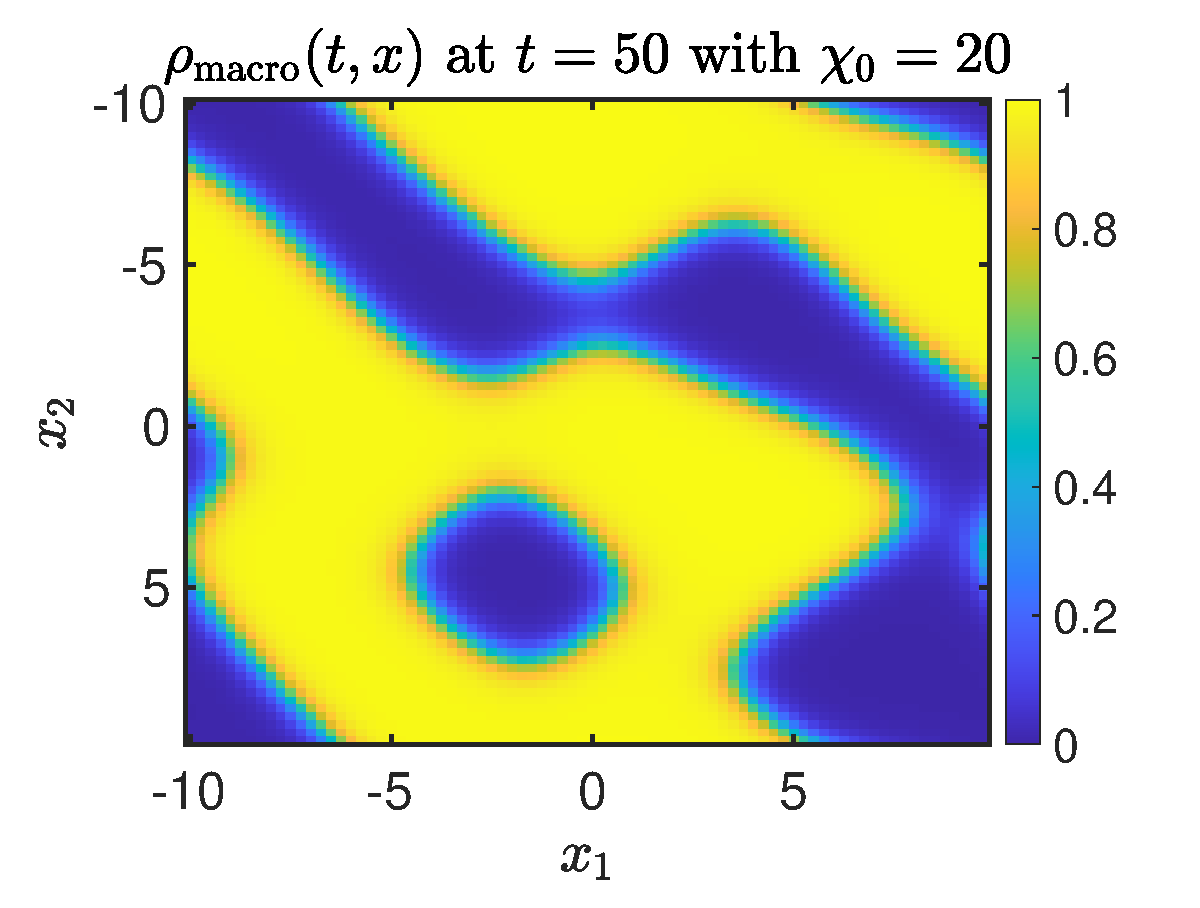
\includegraphics[scale = 0.2]{sol2D_A_20_T_50.eps}
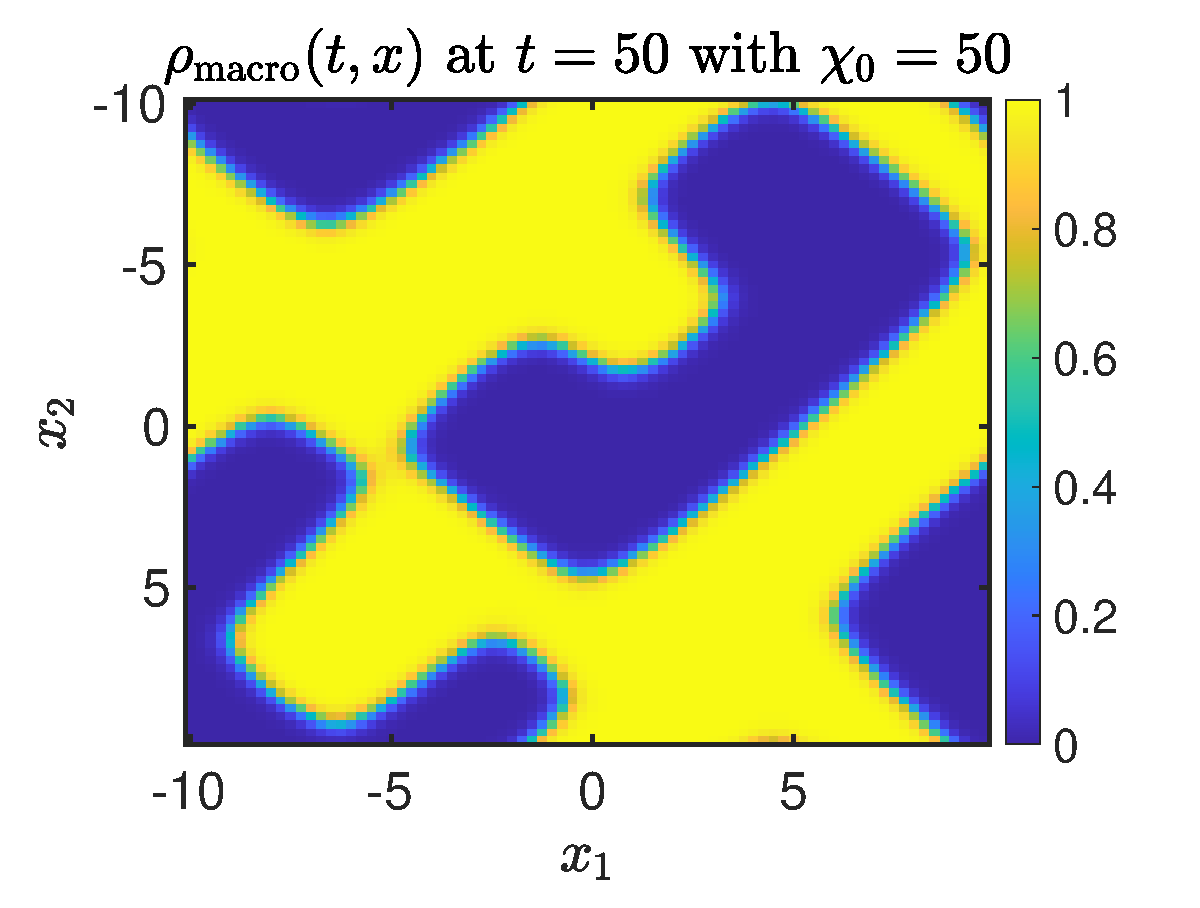
\includegraphics[scale = 0.2]{sol2D_A_50_T_50.eps}
}
\caption{Plots of density $\rho_\textnormal{macro}(t,\mathbf{x})$ at $t=5,\ 20,\ 50$ (from top to bottom) with $\chi_0=6,\ 20,\ 50$ (from left to right), respectively.}
\label{fig:2D_macro}
\end{figure}

% \begin{figure}[tbhp]
% \centerline{
% 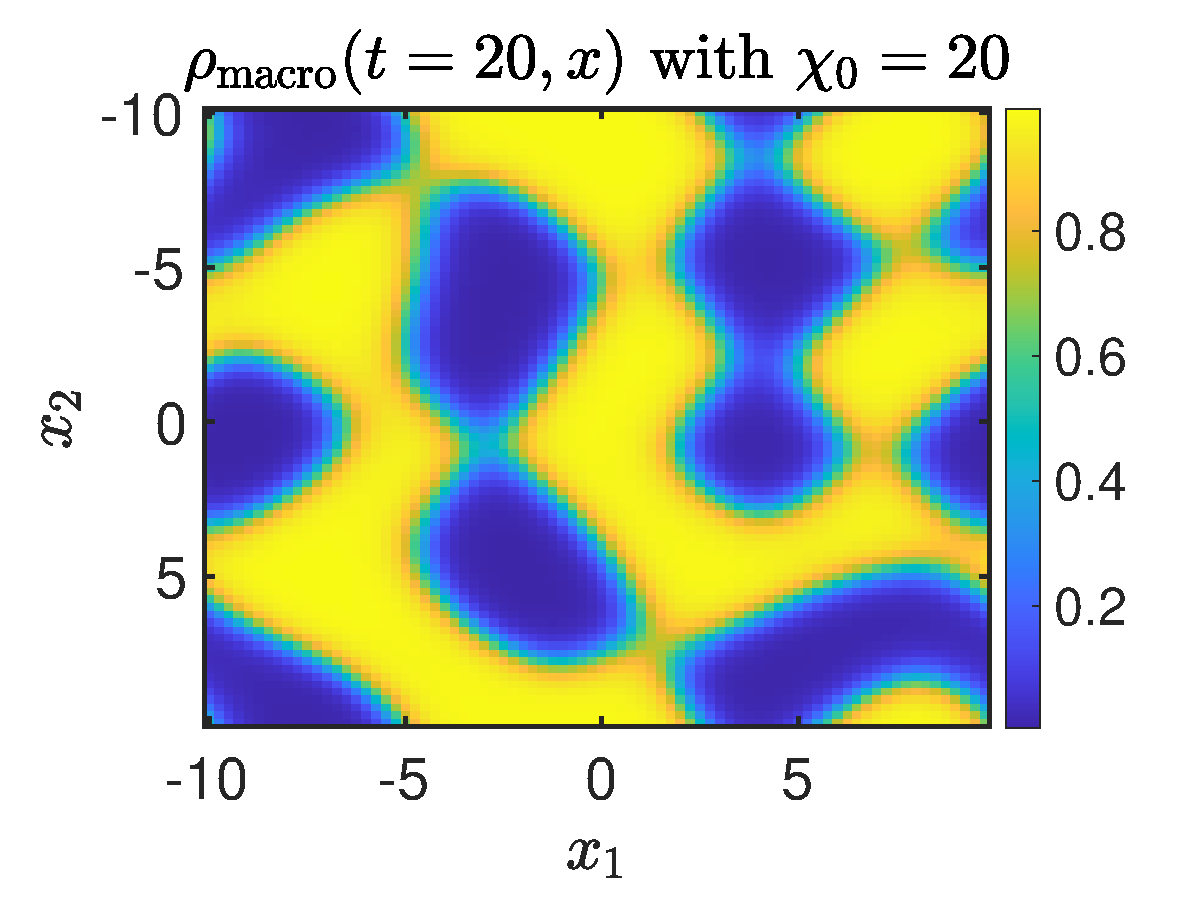
\includegraphics[scale = 0.2]{sol_A_20_T_20_macro_Init_1.eps}
% 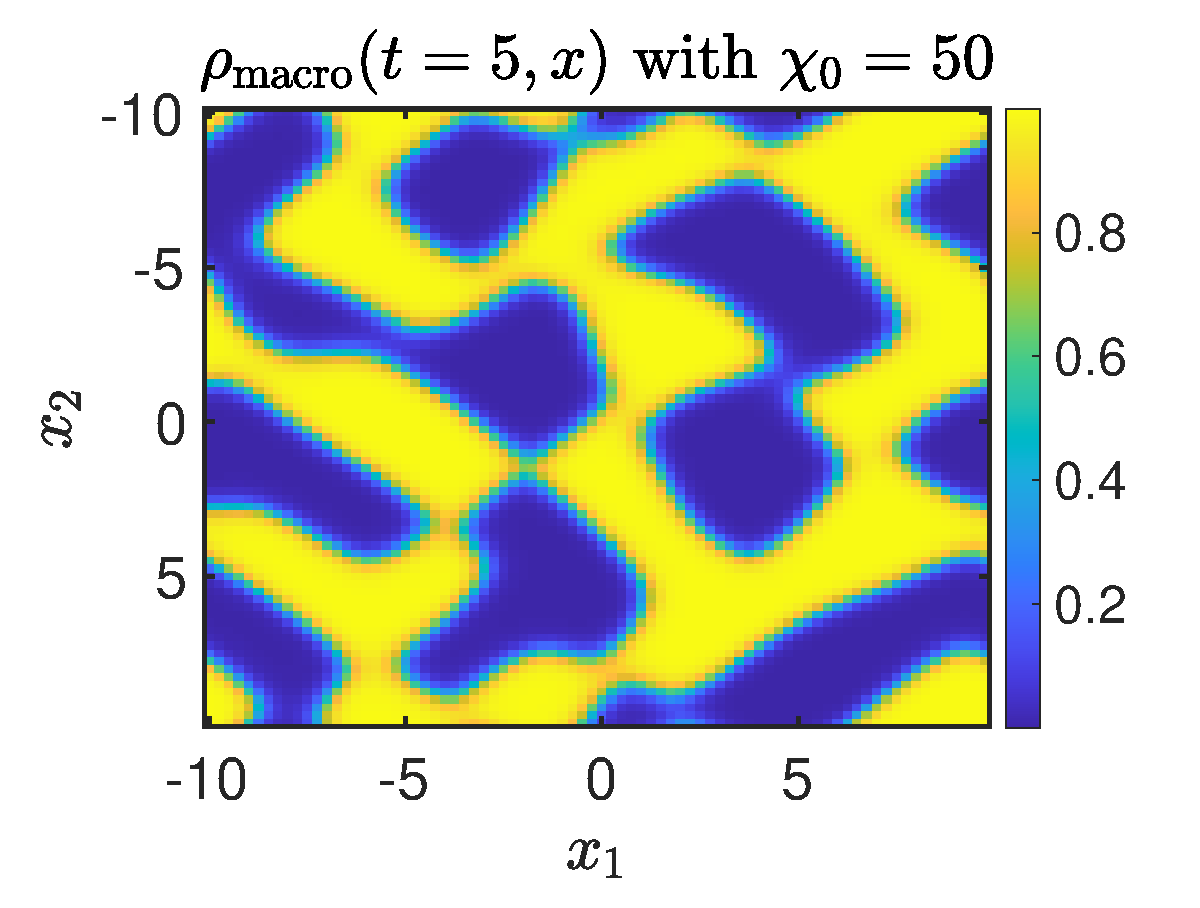
\includegraphics[scale = 0.2]{sol_A_50_T_5_macro_Init_1.eps}
% 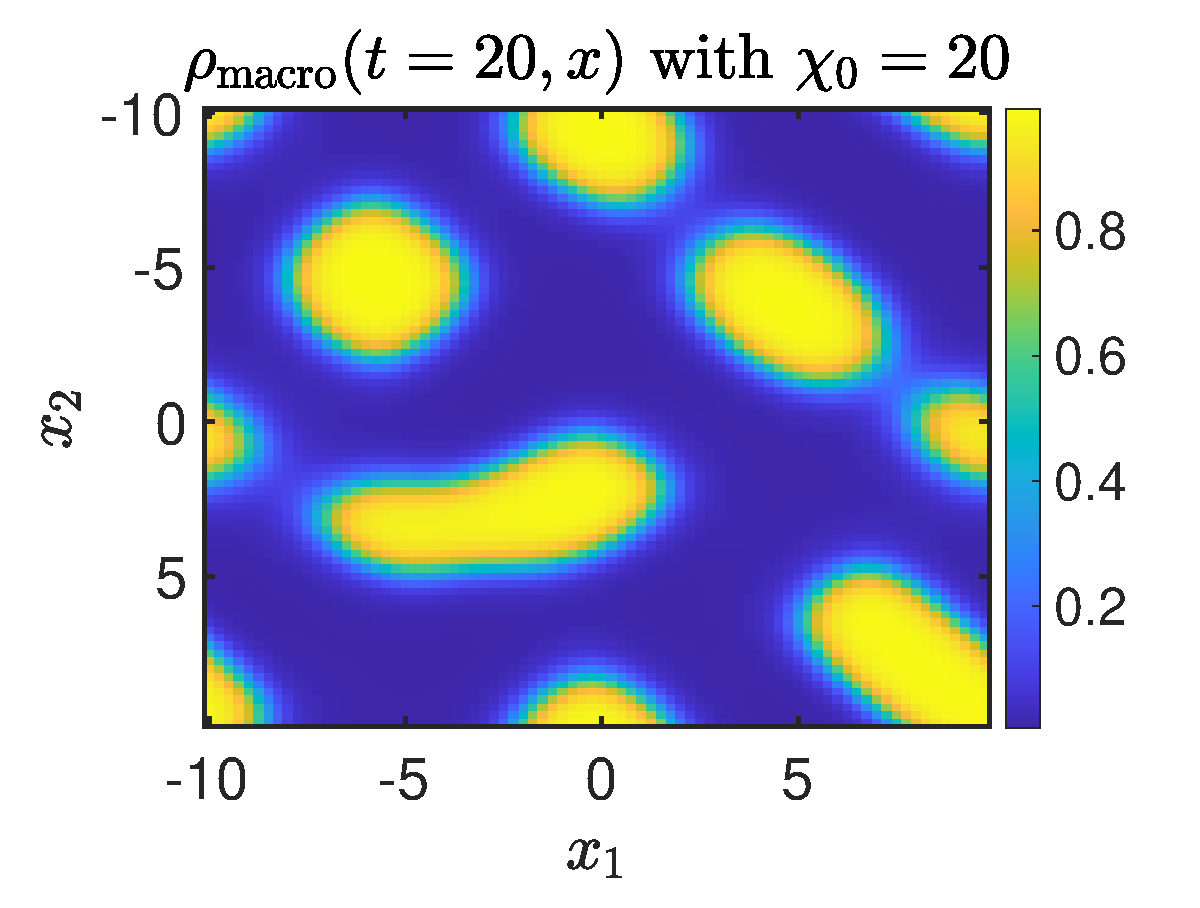
\includegraphics[scale = 0.2]{sol_A_20_T_20_macro_Init_10.eps}
% 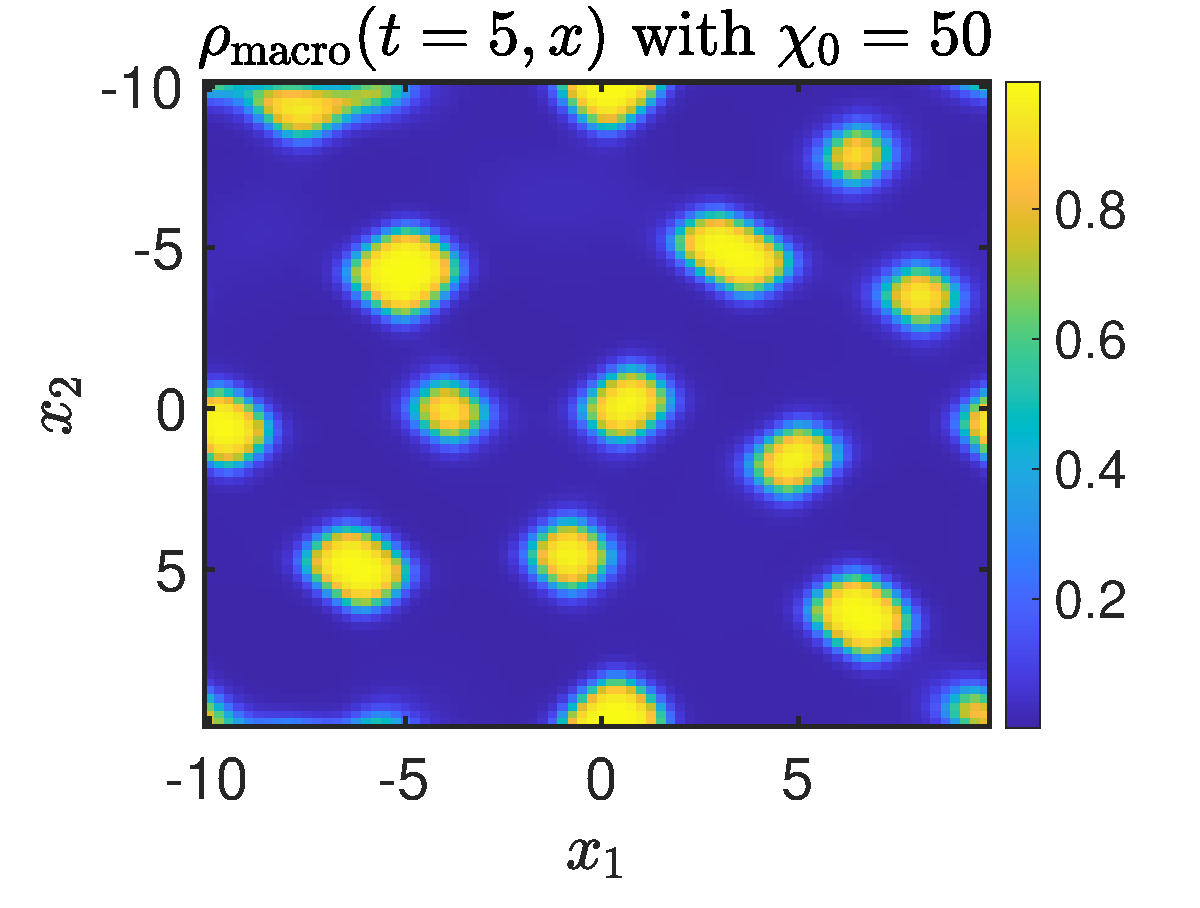
\includegraphics[scale = 0.2]{sol_A_50_T_5_macro_Init_10.eps}
% }

% \centerline{
% 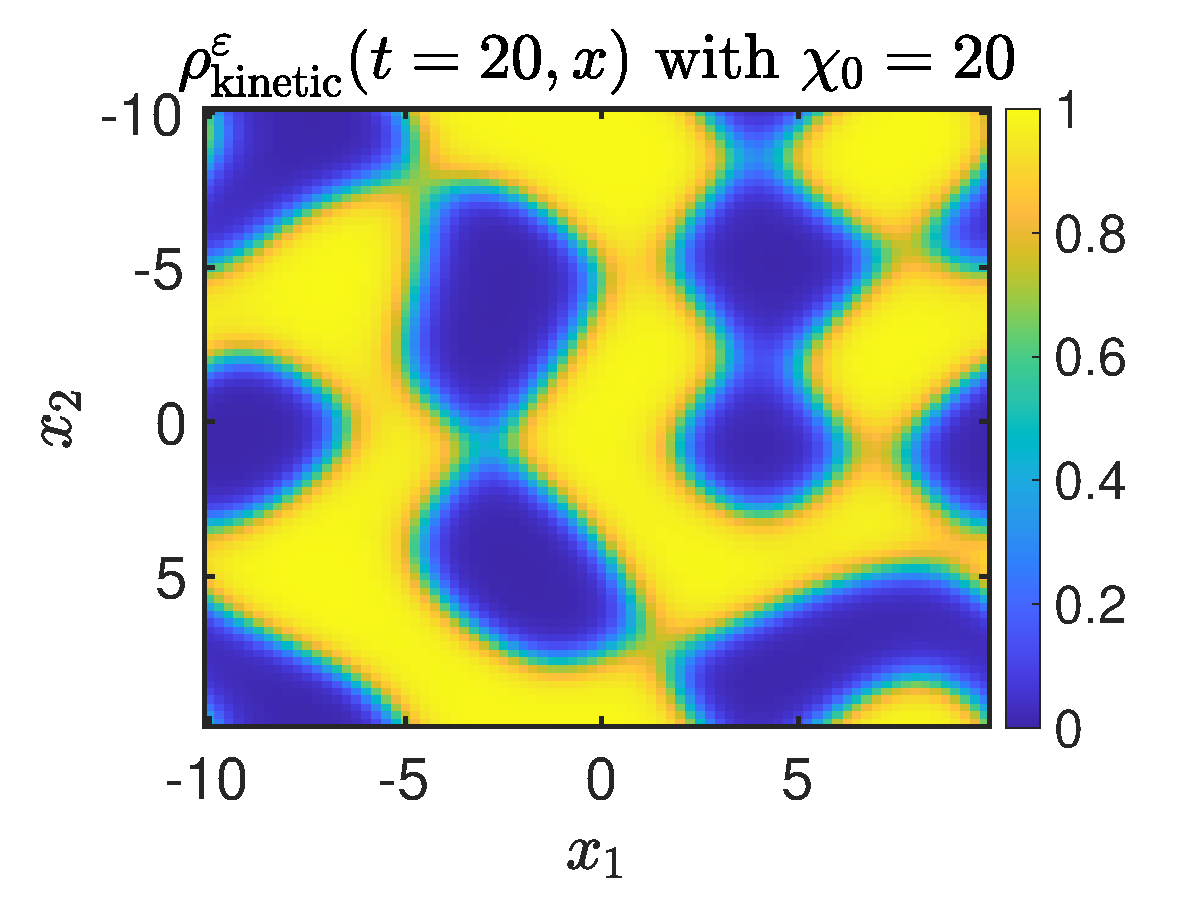
\includegraphics[scale = 0.2]{sol_A_20_T_20_eps_1e-2_Init_1.eps}
% 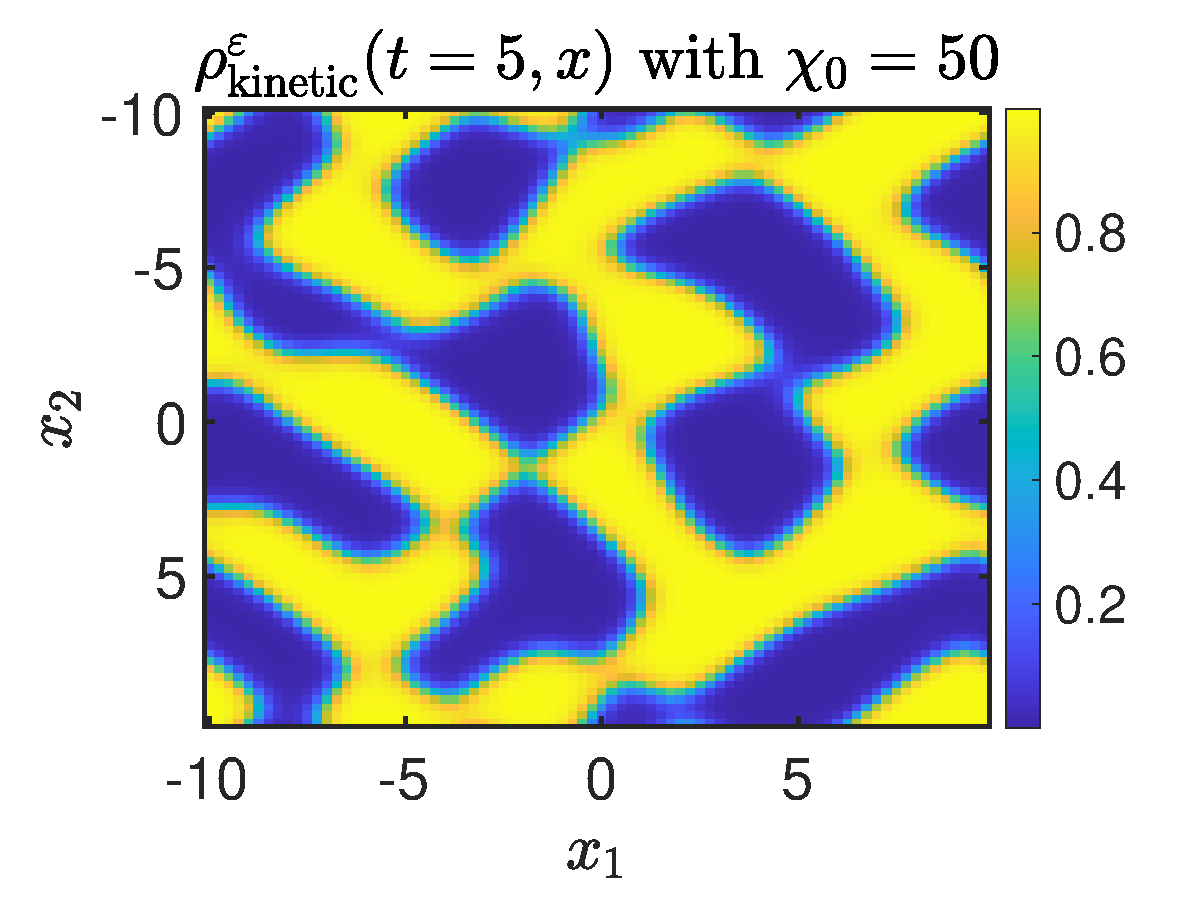
\includegraphics[scale = 0.2]{sol_A_50_T_5_eps_1e-2_Init_1_check.eps}
% 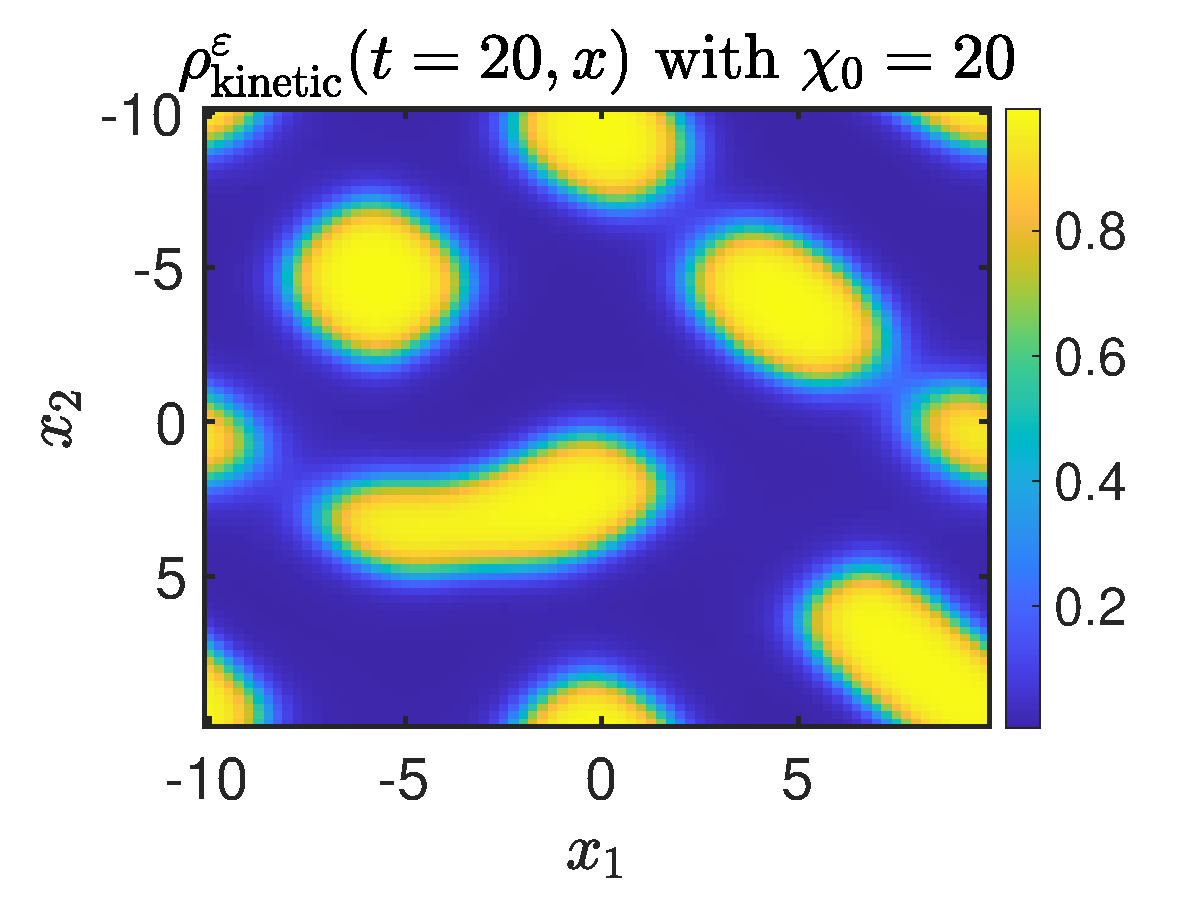
\includegraphics[scale = 0.2]{sol_A_20_T_20_eps_1e-2_Init_10.eps}
% 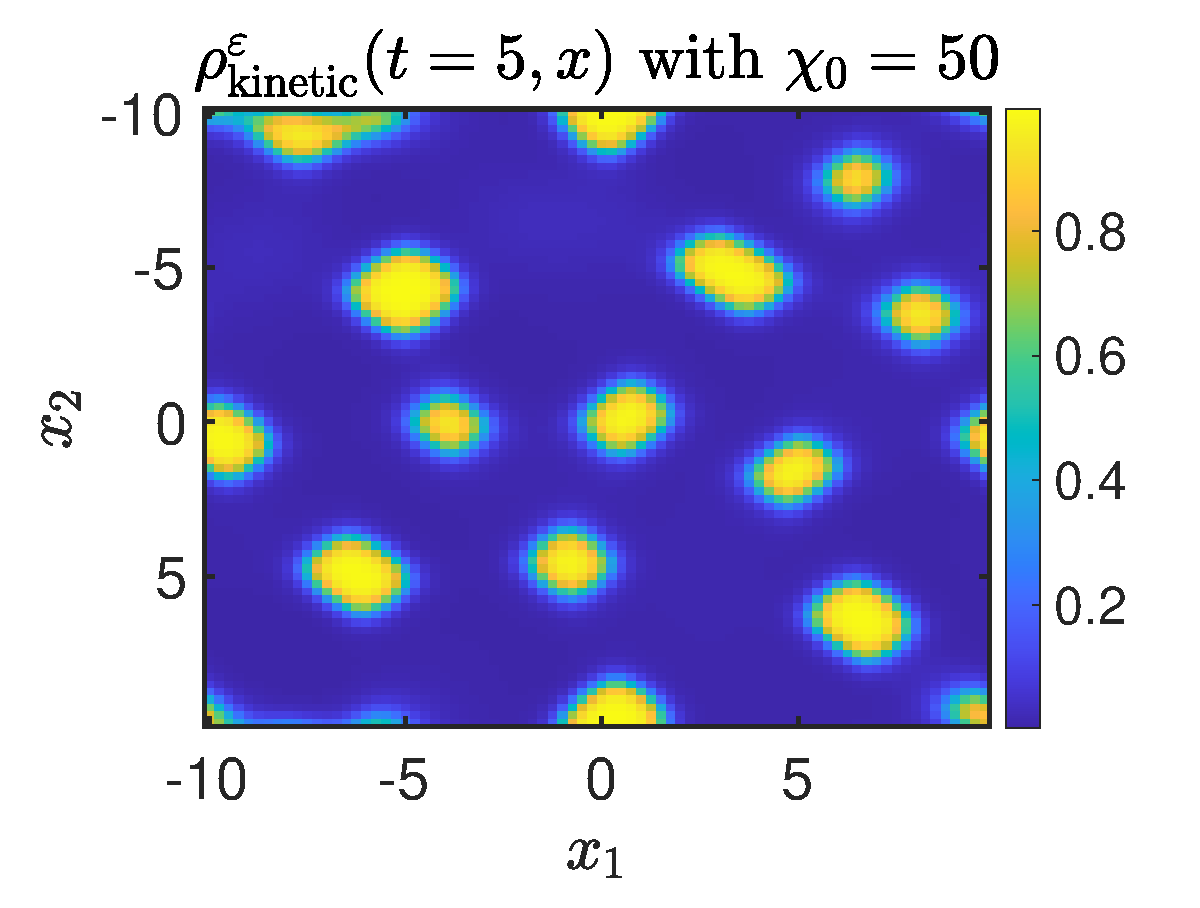
\includegraphics[scale = 0.2]{sol_A_50_T_5_eps_1e-2_Init_10.eps}
% }
% \caption{Comparison between $\rho_\textnormal{macro}(t, \bx)$ (first row) and $\rho_\textnormal{kinetic}^{\varepsilon}(t, \bx)$ with $\varepsilon=10^{-2}$ (second row) for different initial conditions $\rho_0\approx 0.5$ (first two columns) and $\rho_0\approx0.1$ (last two columns) and different values of the chemotactic sensitivity $\chi_0=20$, (columns 1 and 3) and $\chi_0=50$ (columns 2 and 4). }
% \label{fig:2D_compare}
% \end{figure}

\begin{figure}[tbhp]
\centerline{
% 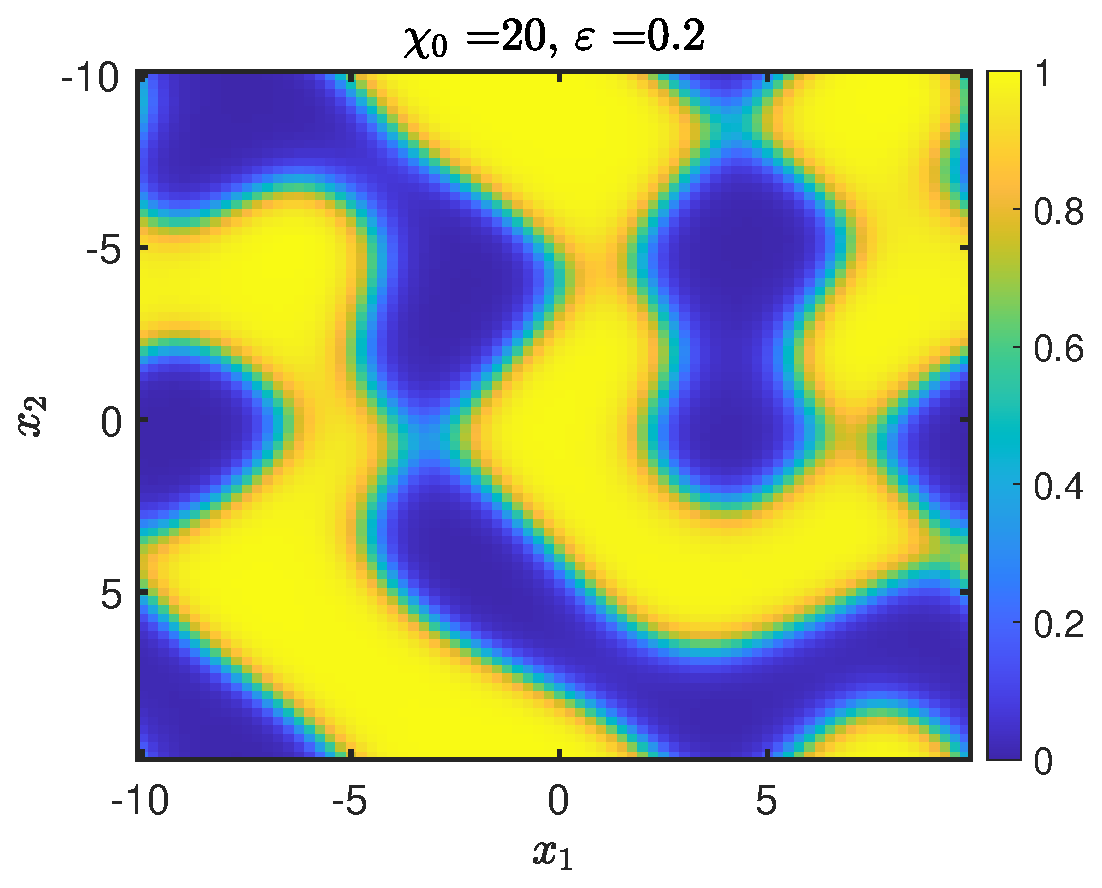
\includegraphics[scale = 0.2]{Fig_2D_A_20_eps_2e-01_T_20_init_1.eps}
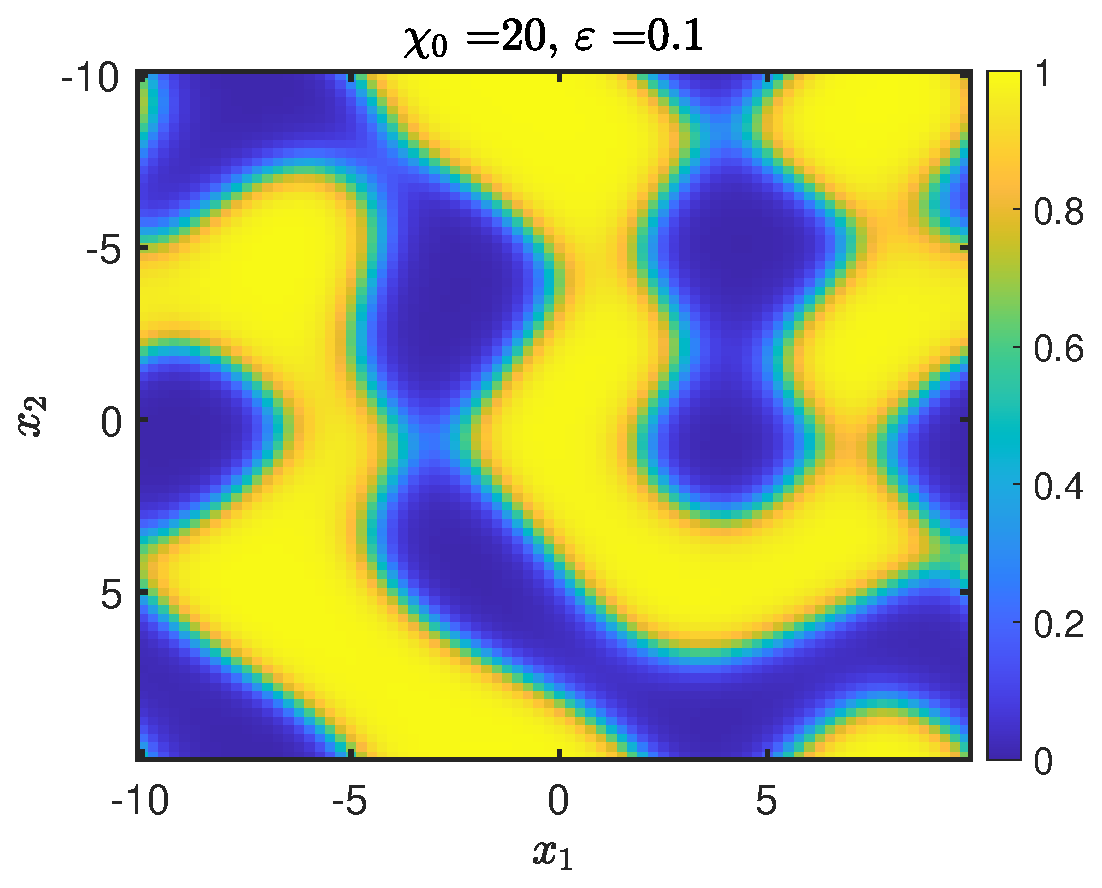
\includegraphics[scale = 0.2]{Fig_2D_A_20_eps_1e-01_T_20_init_1.eps}
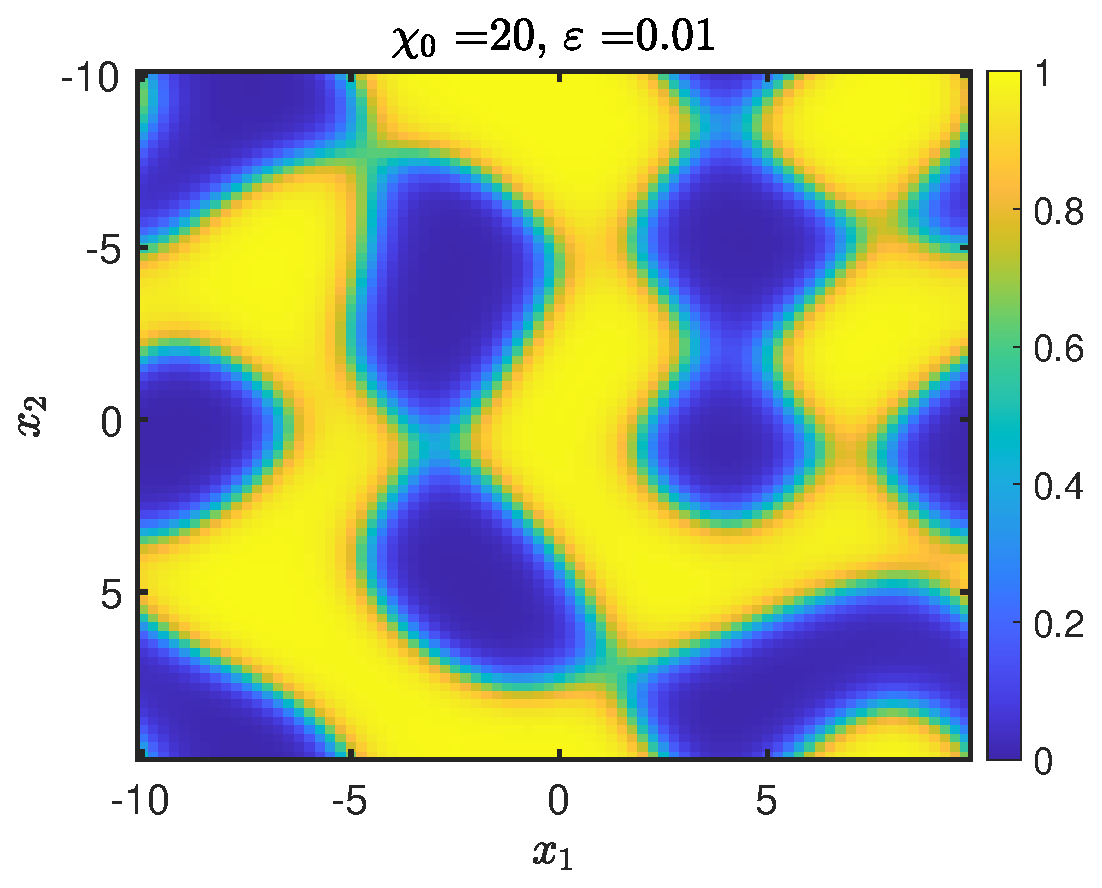
\includegraphics[scale = 0.2]{Fig_2D_A_20_eps_1e-02_T_20_init_1.eps}
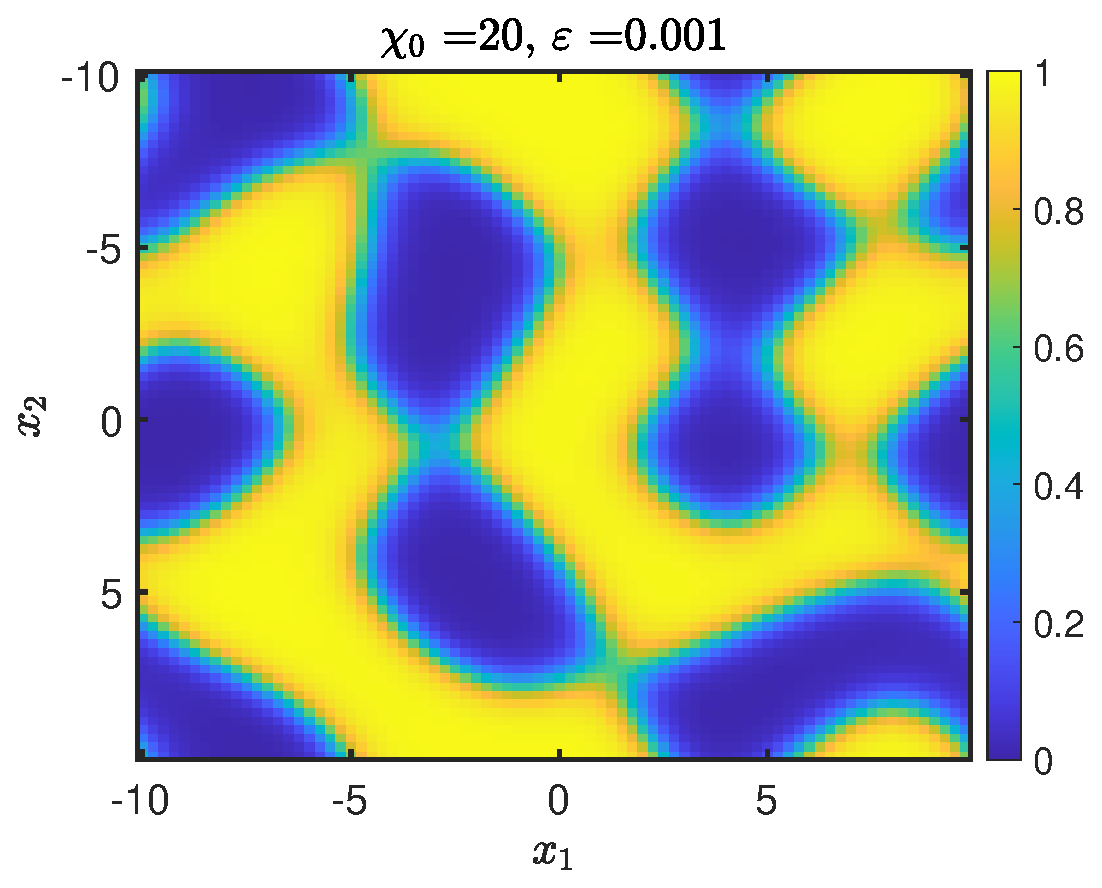
\includegraphics[scale = 0.2]{Fig_2D_A_20_eps_1e-03_T_20_init_1.eps}
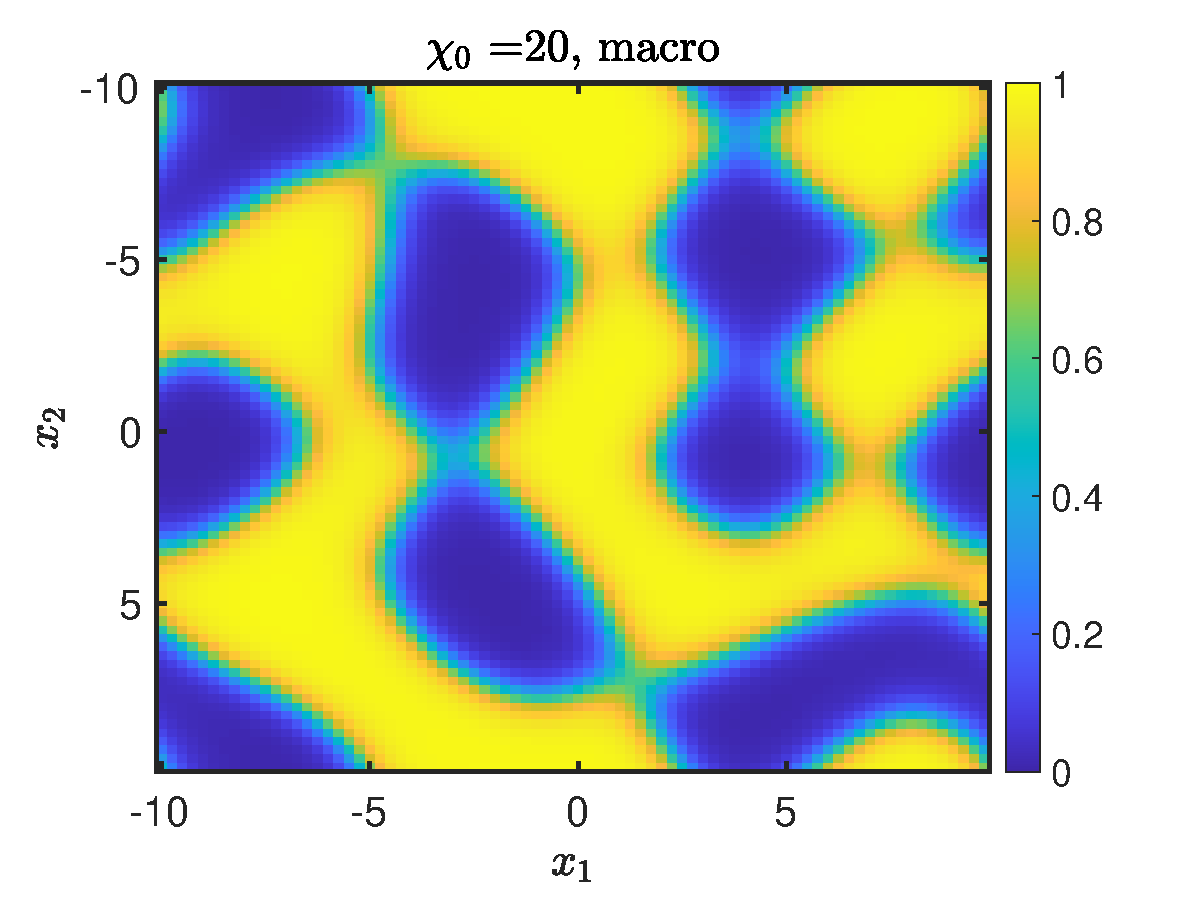
\includegraphics[scale = 0.2]{sol2D_A_20_T_20_init_1.eps}
}
\centerline{
% 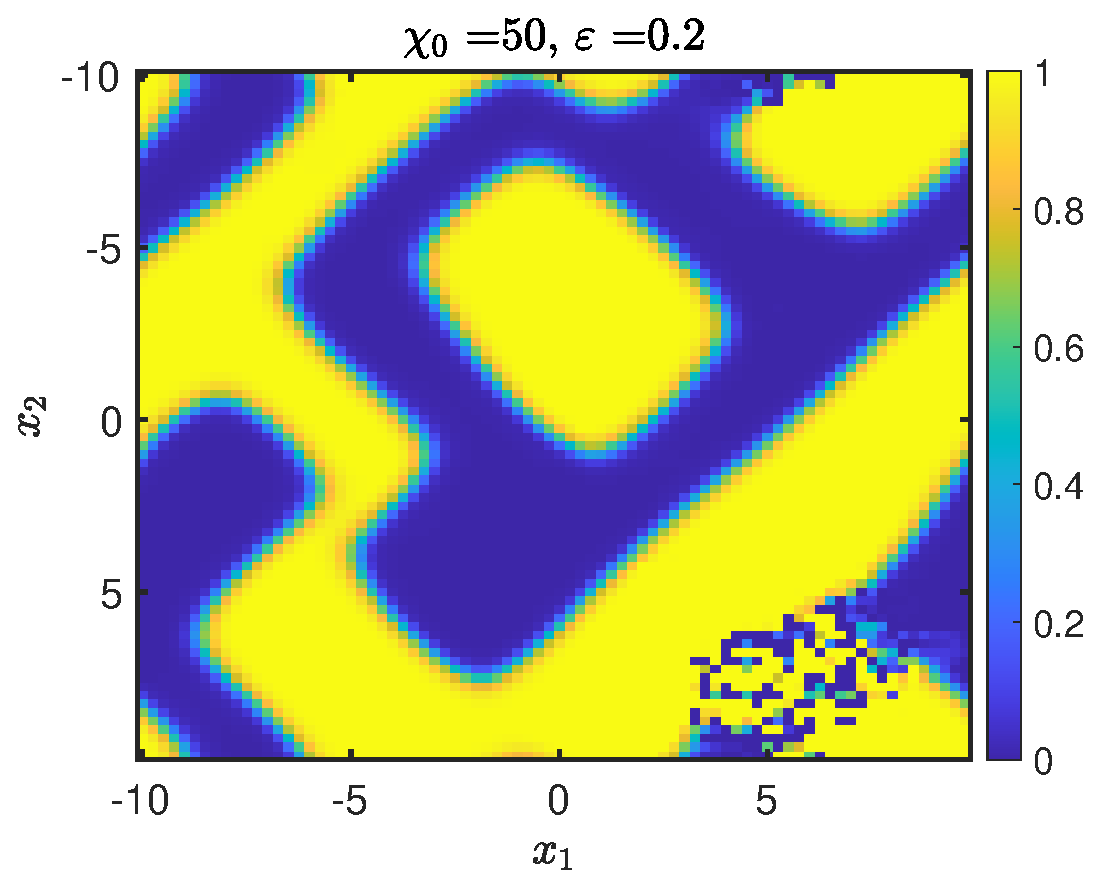
\includegraphics[scale = 0.2]{Fig_2D_A_50_eps_2e-01_T_20_init_1.eps}
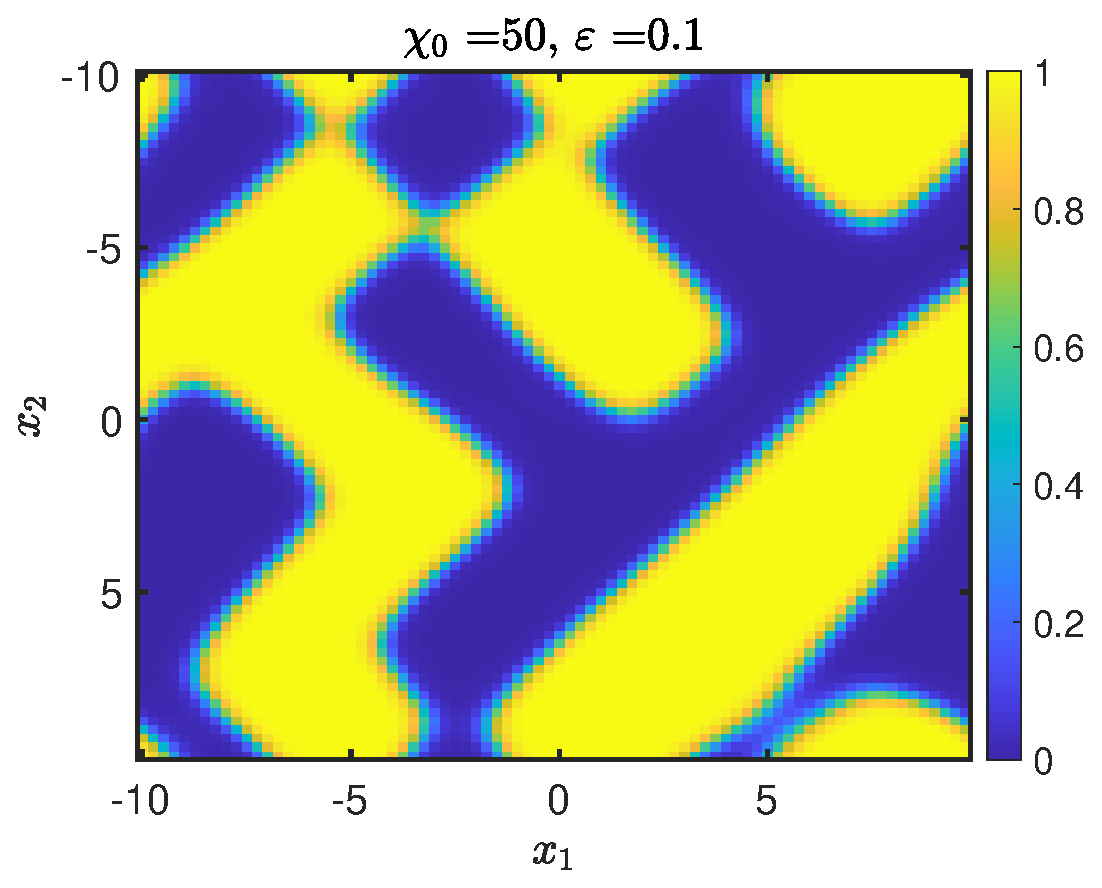
\includegraphics[scale = 0.2]{Fig_2D_A_50_eps_1e-01_T_20_init_1.eps}
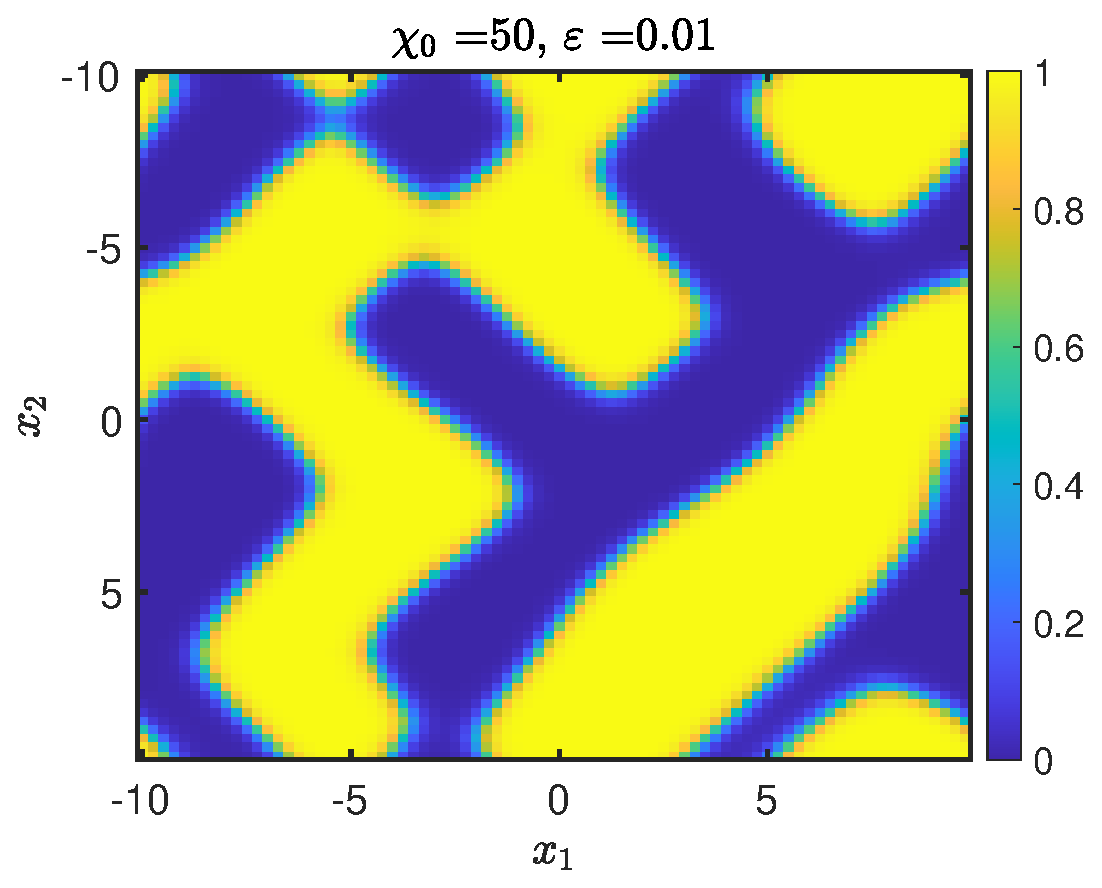
\includegraphics[scale = 0.2]{Fig_2D_A_50_eps_1e-02_T_20_init_1.eps}
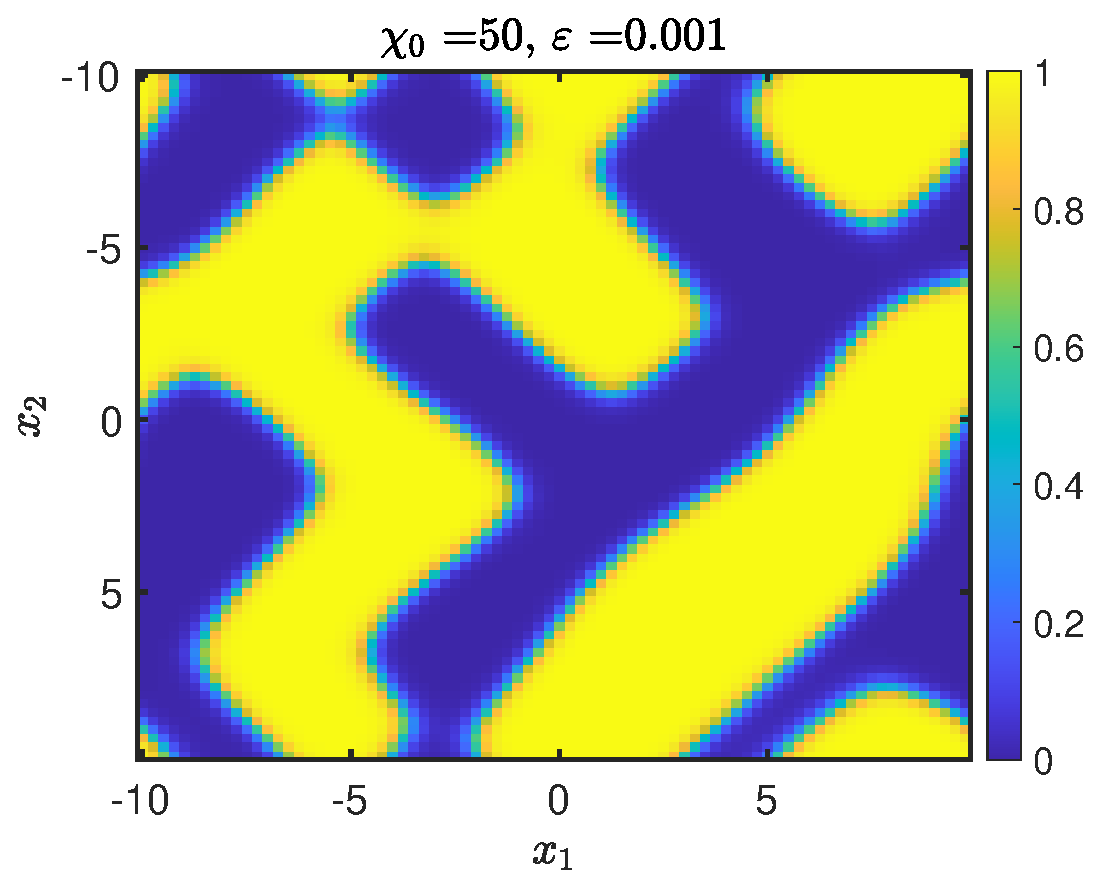
\includegraphics[scale = 0.2]{Fig_2D_A_50_eps_1e-03_T_20_init_1.eps}
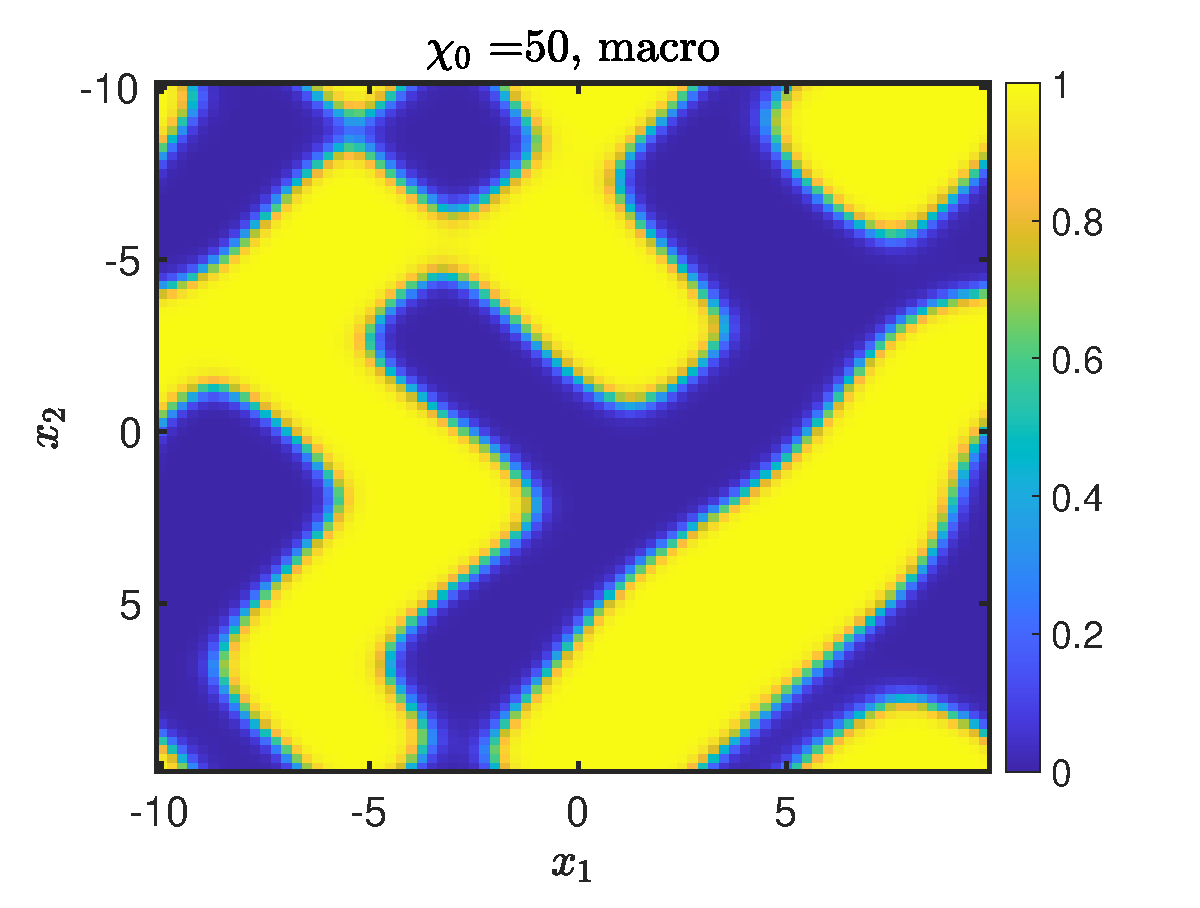
\includegraphics[scale = 0.2]{sol2D_A_50_T_20_init_1.eps}
}
\centerline{
% 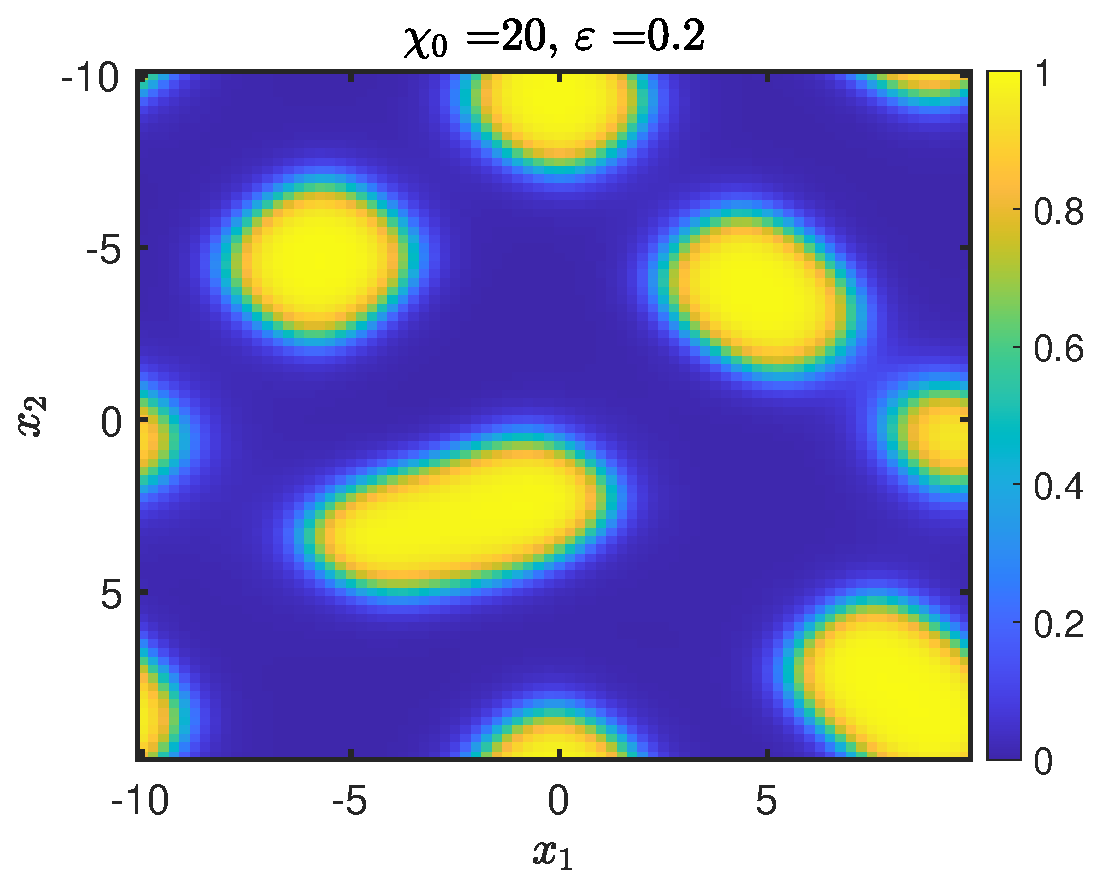
\includegraphics[scale = 0.2]{Fig_2D_A_20_eps_2e-01_T_20_init_10.eps}
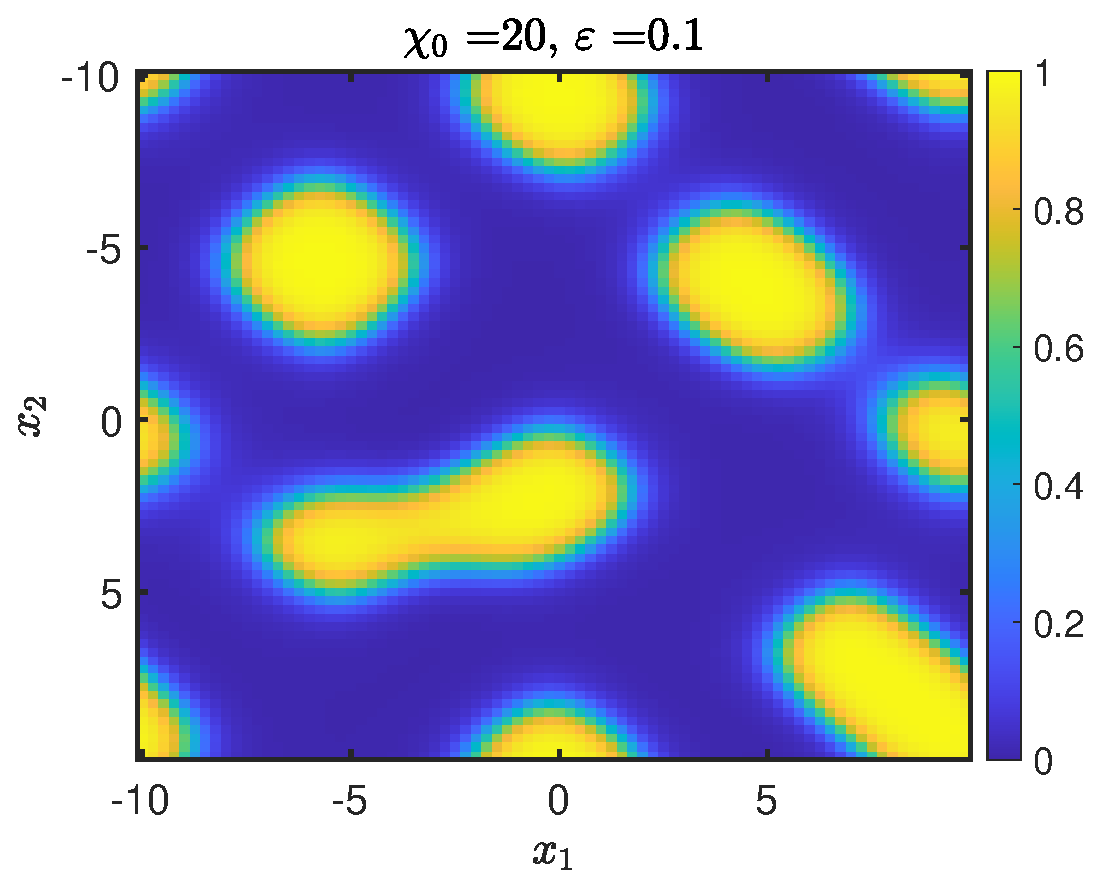
\includegraphics[scale = 0.2]{Fig_2D_A_20_eps_1e-01_T_20_init_10.eps}
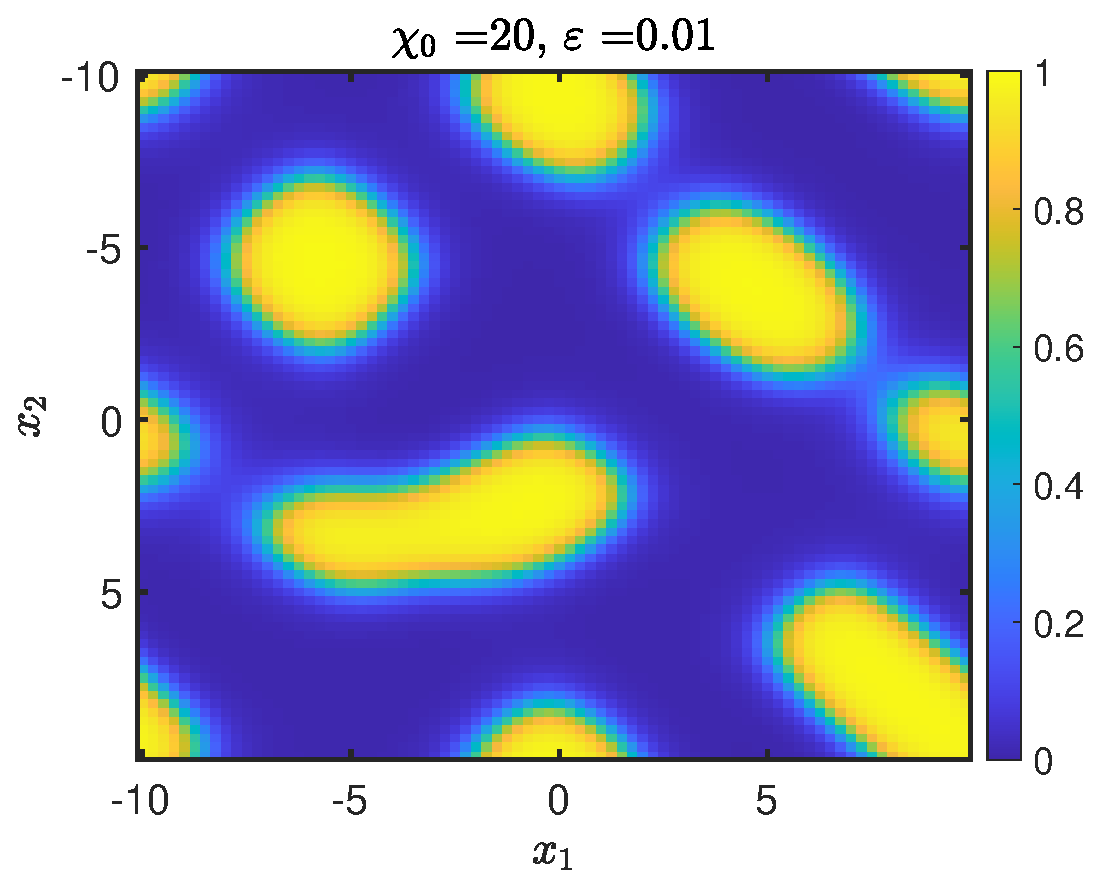
\includegraphics[scale = 0.2]{Fig_2D_A_20_eps_1e-02_T_20_init_10.eps}
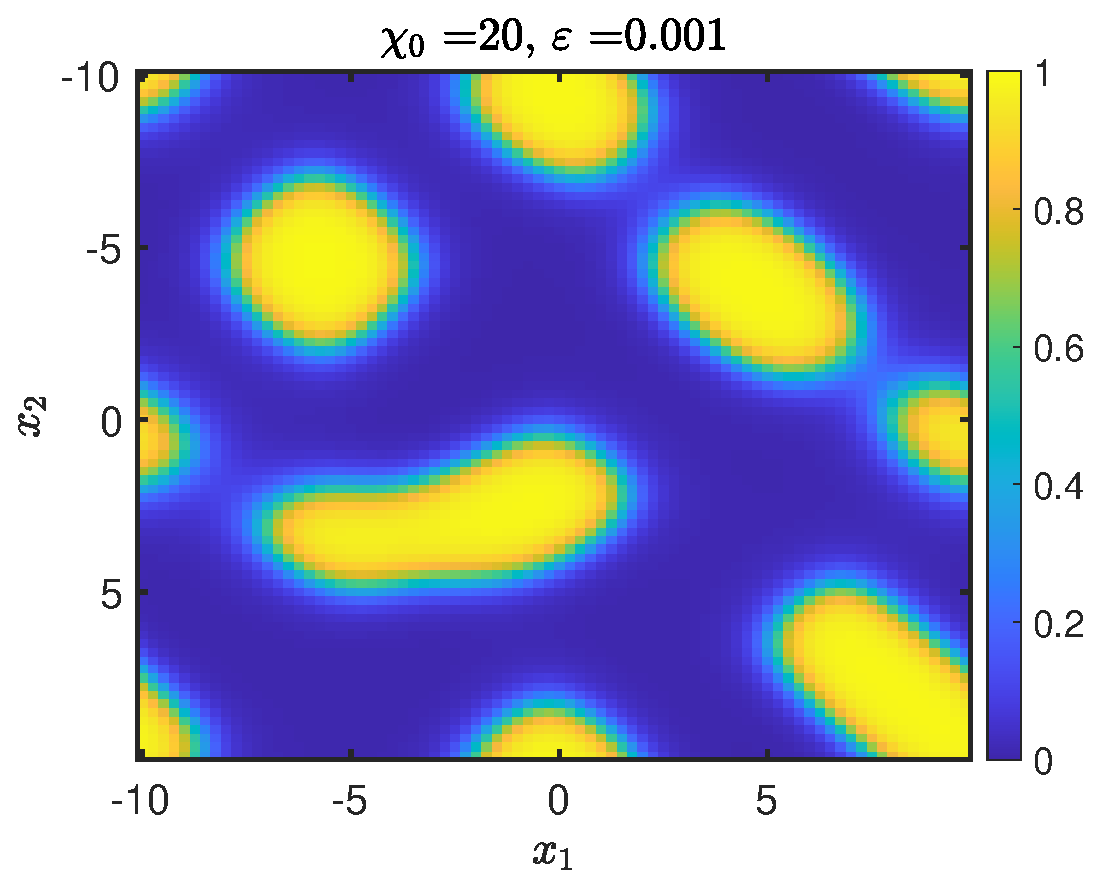
\includegraphics[scale = 0.2]{Fig_2D_A_20_eps_1e-03_T_20_init_10.eps}
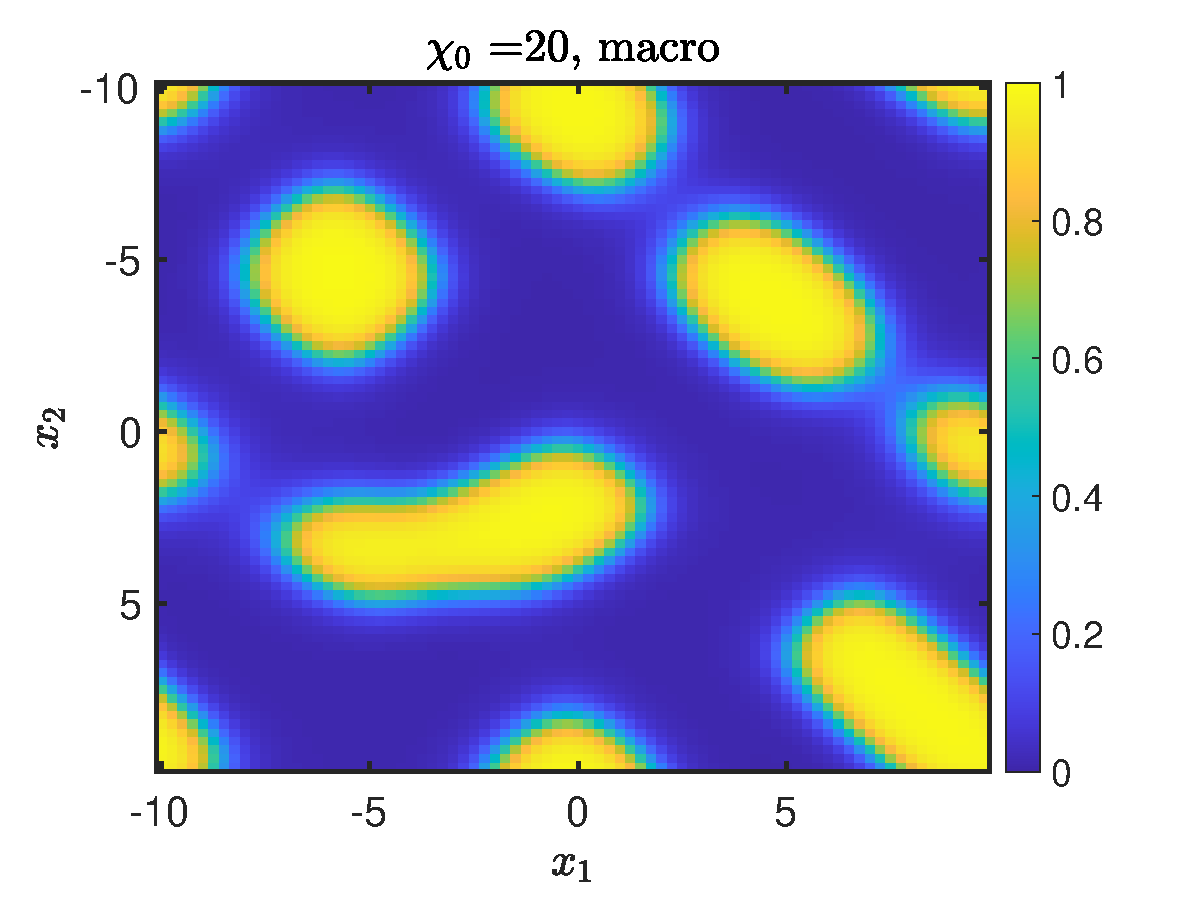
\includegraphics[scale = 0.2]{sol2D_A_20_T_20_init_10.eps}
}
\centerline{
% 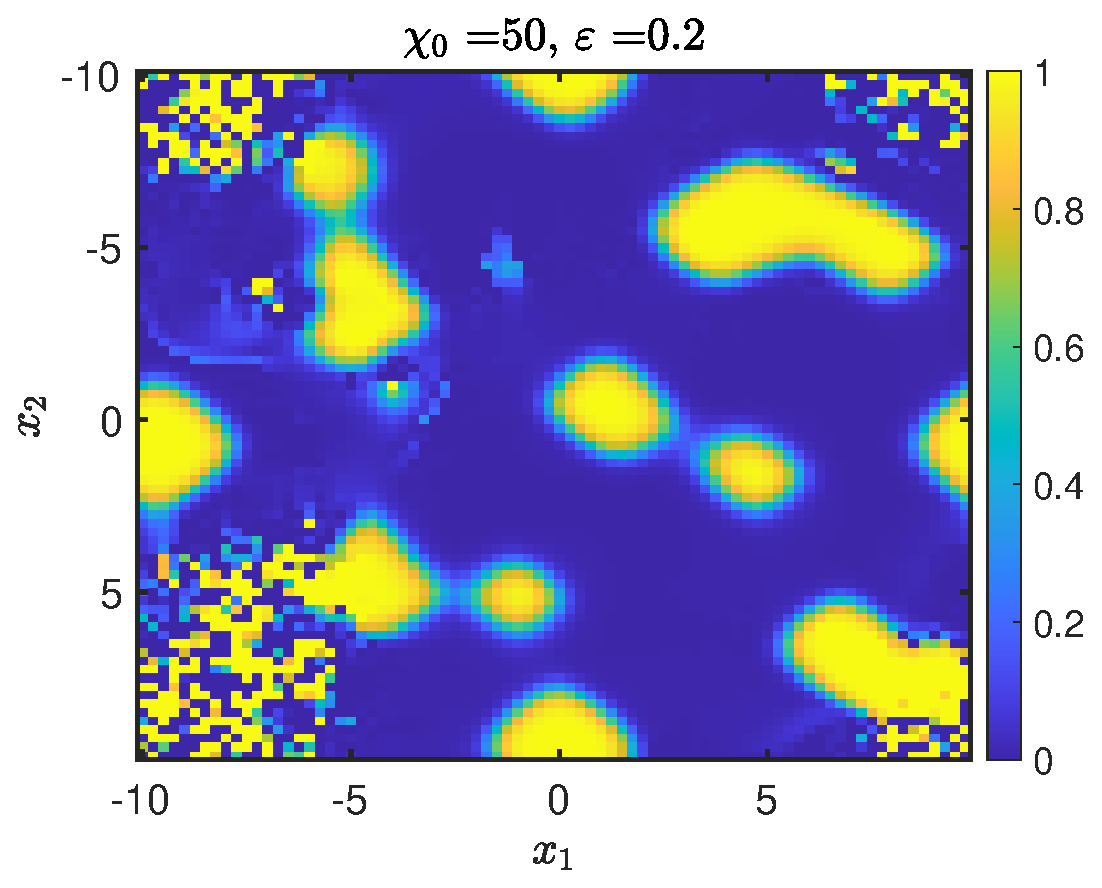
\includegraphics[scale = 0.2]{Fig_2D_A_50_eps_2e-01_T_20_init_10.eps}
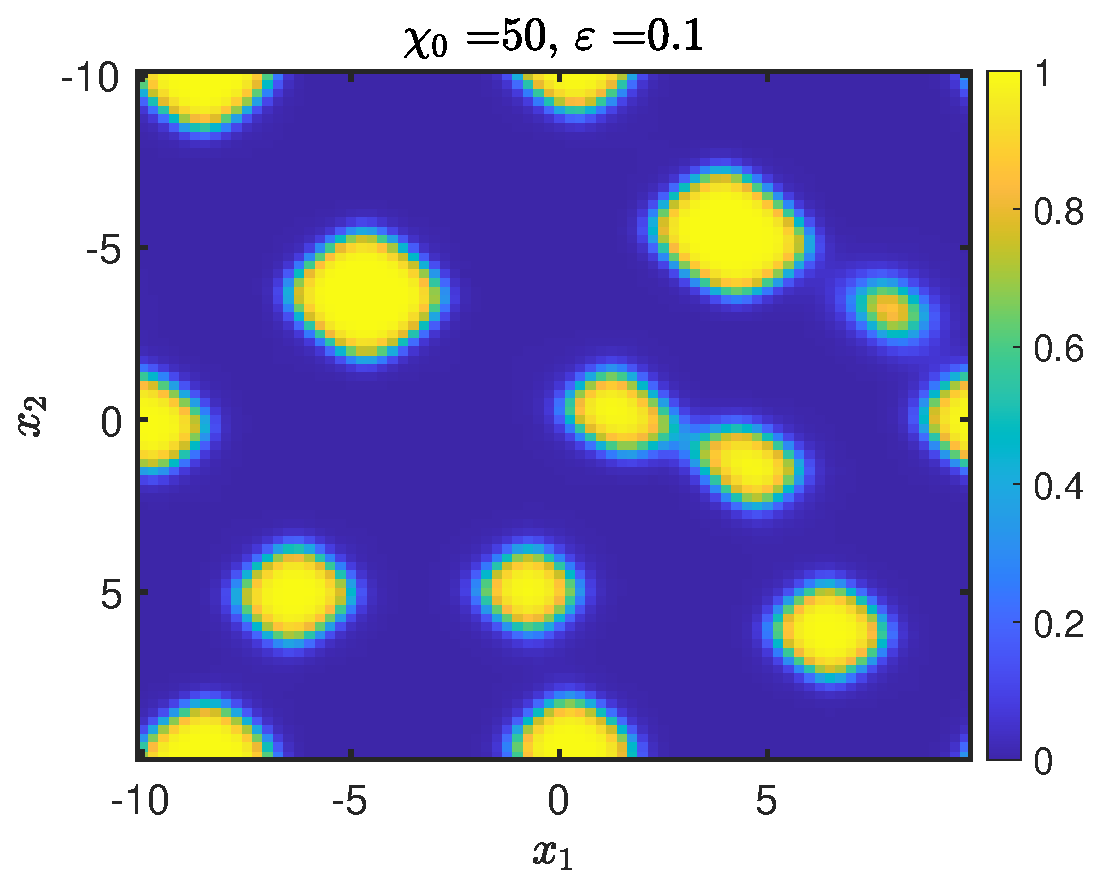
\includegraphics[scale = 0.2]{Fig_2D_A_50_eps_1e-01_T_20_init_10.eps}
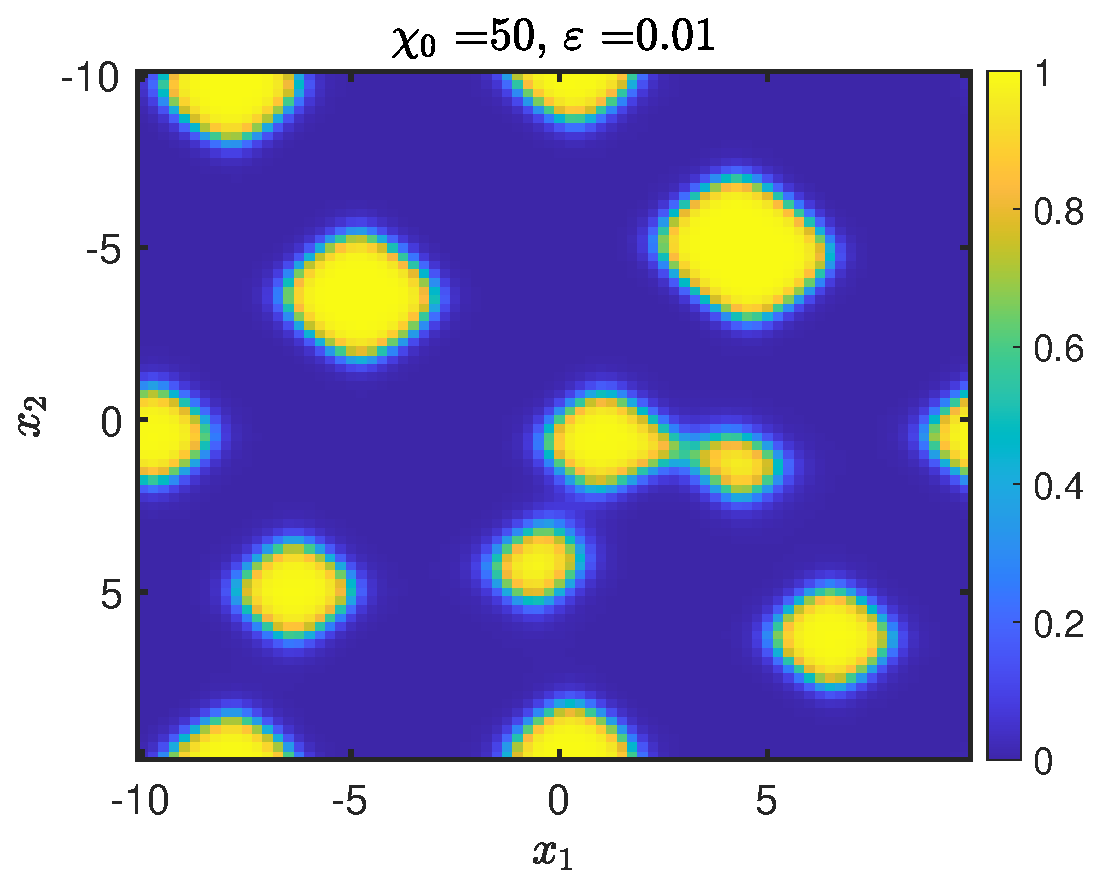
\includegraphics[scale = 0.2]{Fig_2D_A_50_eps_1e-02_T_20_init_10.eps}
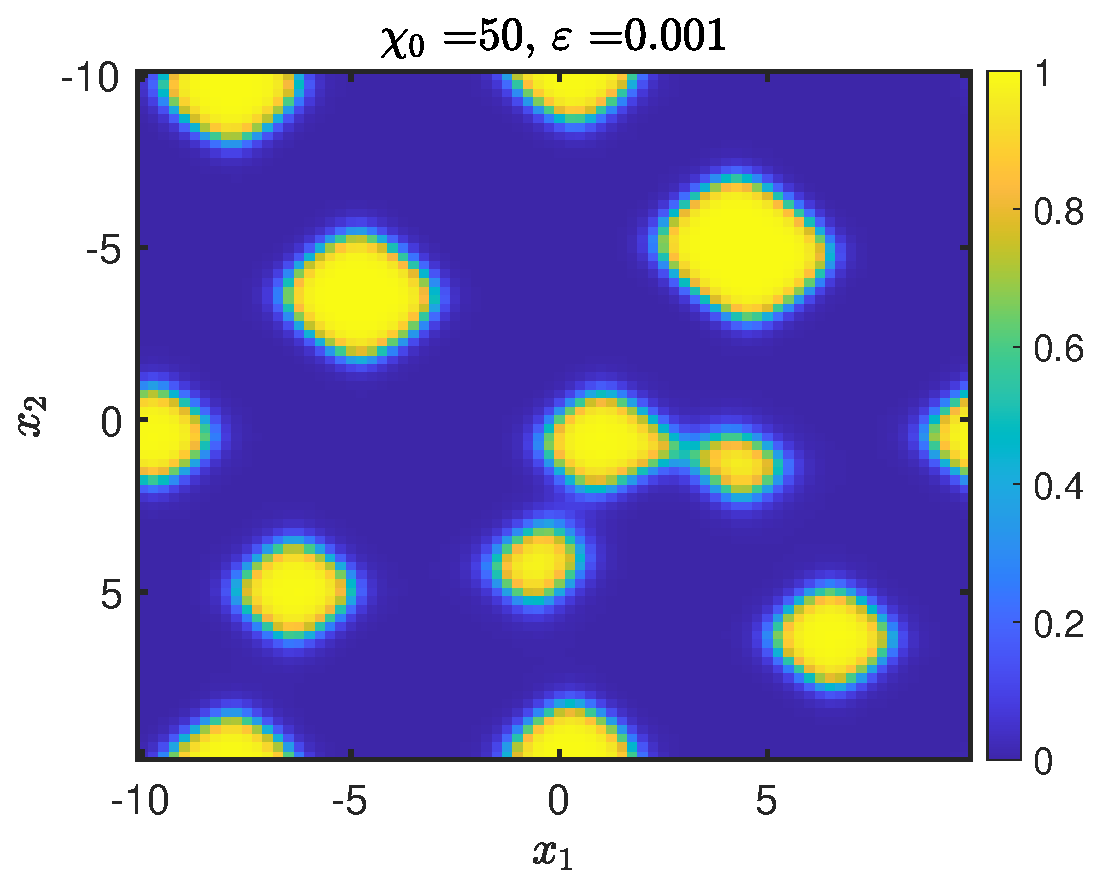
\includegraphics[scale = 0.2]{Fig_2D_A_50_eps_1e-03_T_20_init_10.eps}
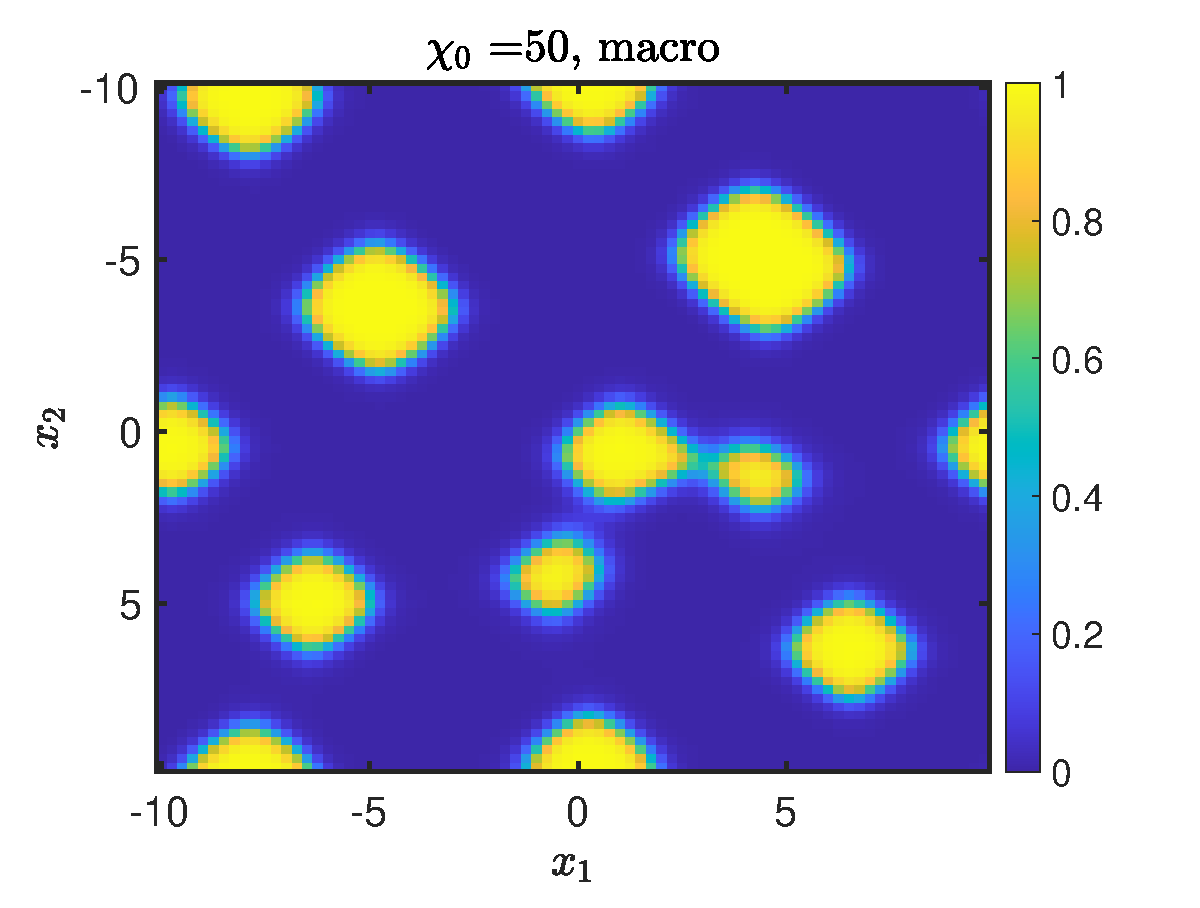
\includegraphics[scale = 0.2]{sol2D_A_50_T_20_init_10.eps}
}
\caption{{\color{blue}Comparison of $\rho_\textnormal{kinetic}^{\varepsilon}(t, \bx)$ for $\varepsilon=10^{-1},10^{-2},10^{-3}$ and $\rho_\textnormal{macro}(t, \bx)$ at $T=20$. In the numerical tests, we set $\chi_0=20$ for the first and third rows, and $\chi_0=50$ for the second and fourth rows. Additionally, the initial values are approximately 0.5 for the first and second rows, and around 0.1 for the third and fourth rows.}}
\label{fig:2D_convergence_sol}
\end{figure}

\begin{figure}[tbhp]
\centerline{
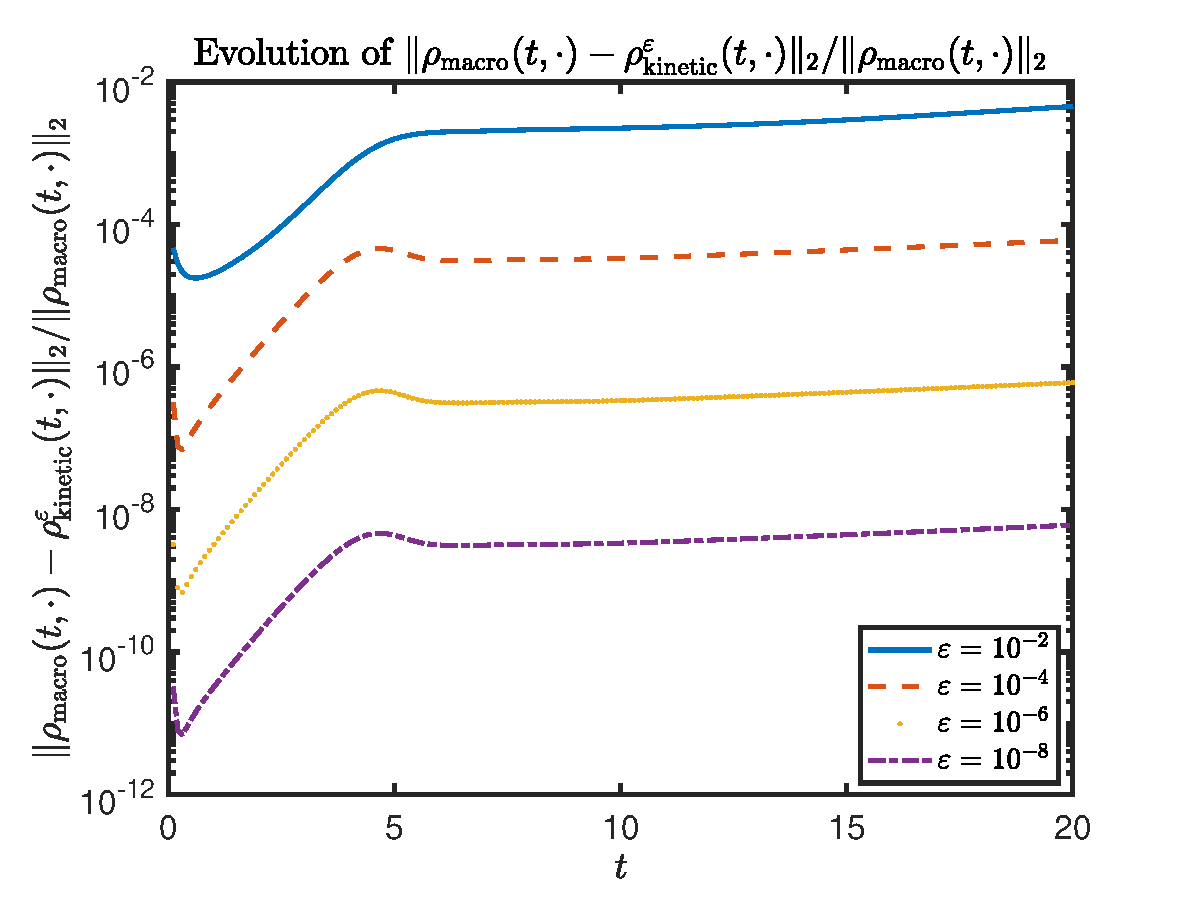
\includegraphics[scale = 0.3]{l2_relative_error_2D_A_20_T_20.eps}
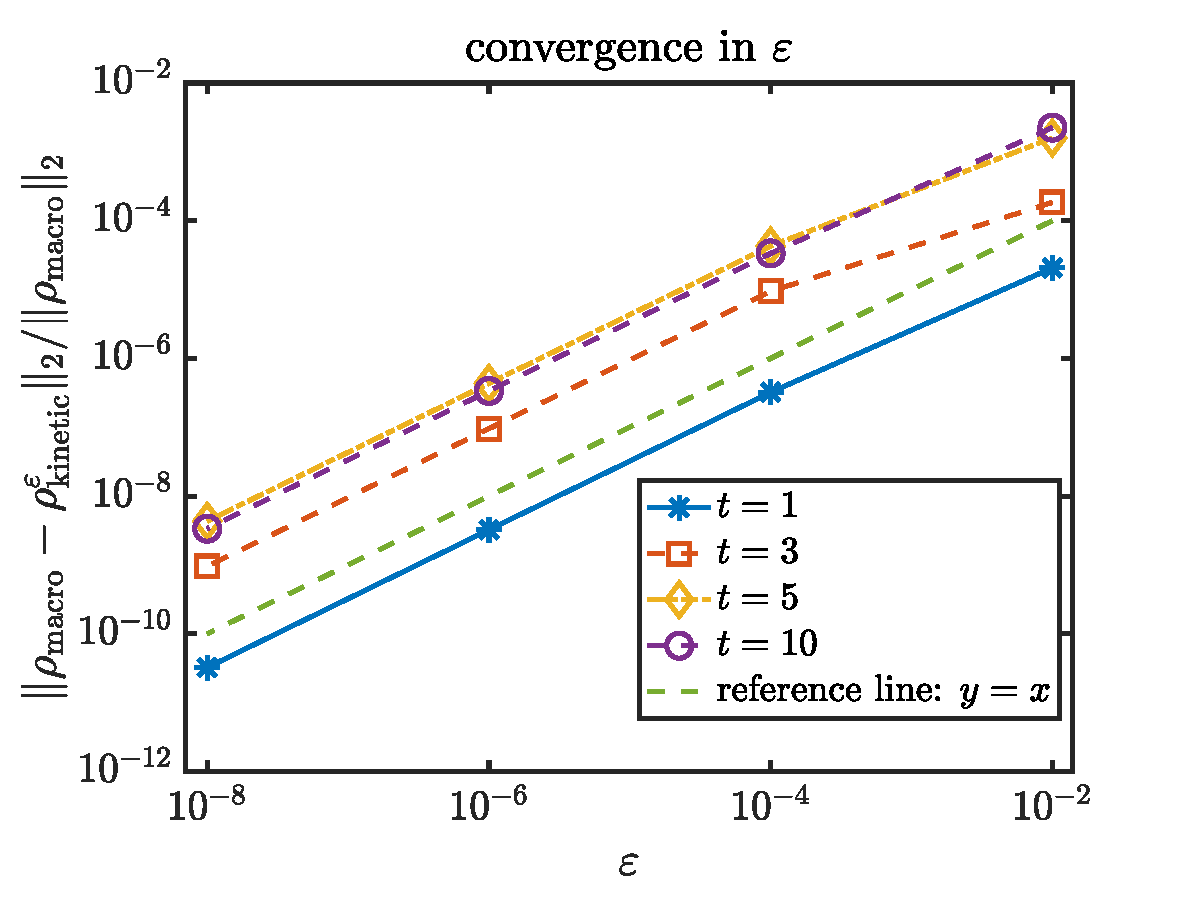
\includegraphics[scale = 0.3]{convergence_vep_2D.eps}
}
\caption{{Left: Evolution of the relative $L_2$-error. Right: } Convergence of the relative $L_2$-error in $\e$ at $t=1,\ 3,\ 5,\ 10$ with $\chi_0=20$ and $\dt=10^{-2}$.}
\label{fig:2D_convergence}
\end{figure}


\section{Conclusions}

{In this paper we have derived a model for chemotaxis incorporating a density dependence in the chemotactic sensitivity function that takes into account the finite size of the cells and volume limitations. We showed, with formal arguments, that the macroscopic chemotactic system can be seen as the diffusion limit of a kinetic 'velocity-jump' model, provided that both the transport term and the turning operator are density dependent. This derivation provides a more direct interpretation of the diffusion tensor and chemotactic sensitivity in terms of more fundamental characteristics of the motion.

We further studied this macroscopic limit numerically using an asymptotic preserving finite difference scheme based on a micro-macro decomposition of the unknown in the sense of  \cite{LemouMieussens}, a projection technique to obtain
a coupled system of two evolution equations for the microscopic and macroscopic
components, and a suitable semi-implicit time discretization. The scheme was successfully extended to account for nonlinear terms by implicit-explicit discretization in an upwind manner, allowing for accurate approximations in the case of strong chemosensitivity. This scheme enabled us to explore numerically the different behaviours observed by the kinetic and macroscopic models in 1D and 2D, and we showed that both models are in good agreement as the diffusion scaling parameter becomes smaller. Moreover, the numerical simulations of the kinetic model
revealed the same pattern sizes as obtained with the macroscopic model and predicted theoretically, with very good precision as $\e$ goes to zero in the kinetic setting. 

From the modeling perspective, it would be natural to extend the derivation to consider different turning kernels, to take into account cell-cell adhesion or nonlocal movement, for instance. The idea to construct the scheme could be generalized to include these cases, but we stress the fact that the detailed discretization is problem-dependent. %Natural perspectives of these works include a rigorous proof of the uniform stability of our numerical scheme. The difficulty lies in the nonlinearity of the chemosensitivity term. 
Moreover, the rigorous derivation of volume-filling chemotactic equations from stochastic processes of interacting populations could be considered by adapting ideas from \cite{stevens2000derivation} for instance. 
}


\appendix


\section{A finite difference scheme for the 2D kinetic model} \label{sec:appendix-FD-2D}
The finite difference scheme \eqref{eq:scheme} can be generalized to multi-dimensional problems where a tensor product grid is applied. 
Here we consider the 2D kinetic model with the special choice $\psi_0(v_1,v_2)$ and $\psi_1(v_1, v_2) = \vec{\phi}(v_1,v_2) \cdot \nabla c$, where $\vec{\phi}(v_1,v_2) = (\phi_1(v_1,v_2), \phi_2(v_1,v_2))^T $, 
{ such that 
$D I_2 = \int (\bv\otimes \bv) \psi_0 \diff v_1 \diff v_2$ 
and
$\chi_0 I_2 = \int \bv\otimes \vec{\phi} \diff v_1 \diff v_2$ with $\bv=(v_1, v_2)^T$ and $I_2$ being the 2-dimentional identity matrix. 
}

We introduce the notations  $\rho_{j_1,j_2}^n$, $c_{j_1,j_2}^n$,  $g_{j_1+\frac12,j_2,k_1,k_2}^{(1), n}$ and $g_{j_1,j_2+\frac12,k_1,k_2}^{(2), n}$ to be the numerical approximations of $\rho(t_n,x_{j_1}, x_{j_2})$, $c(t_n,x_{j_1}, x_{j_2})$, $g(t_n, x_{j_1+\frac12}, x_{j_2}, v_{k_1}, v_{k_2})$ and 
$g(t_n, x_{j_1}, x_{j_2+\frac12}, v_{k_1}, v_{k_2})$, respectively. 
The approximations of $\rho(t, \mathbf{x})$ at half grid points such as $(x_{j_1}, x_{j_2+\frac12})$ can be then easily approximated by the average $\bar{\rho}_{j_1, j_2+\frac12} := (\rho_{j_1, j_2} + \rho_{j_1, j_2+1})/2$. 
It is worth noticing that we used different notations for approximating $g(t_n, x_{j_1+\frac12}, x_{j_2}, *, *)$ and $g(t_n, x_{j_1}, x_{j_2+\frac12}, *, *)$ since different upwind discretizations will be used depending on whether the half grid is in $x_1$-direction or $x_2$-direction. 
An illustration of the grids in $\mathbf{x}$-space for computing $\rho(t,\mathbf{x})$ and $g(t,\mathbf{x},\mathbf{v})$ in 1D and 2D can be found in Figure \ref{fig:grid_illstration}. 

\begin{figure}[tbhp]
\centerline{
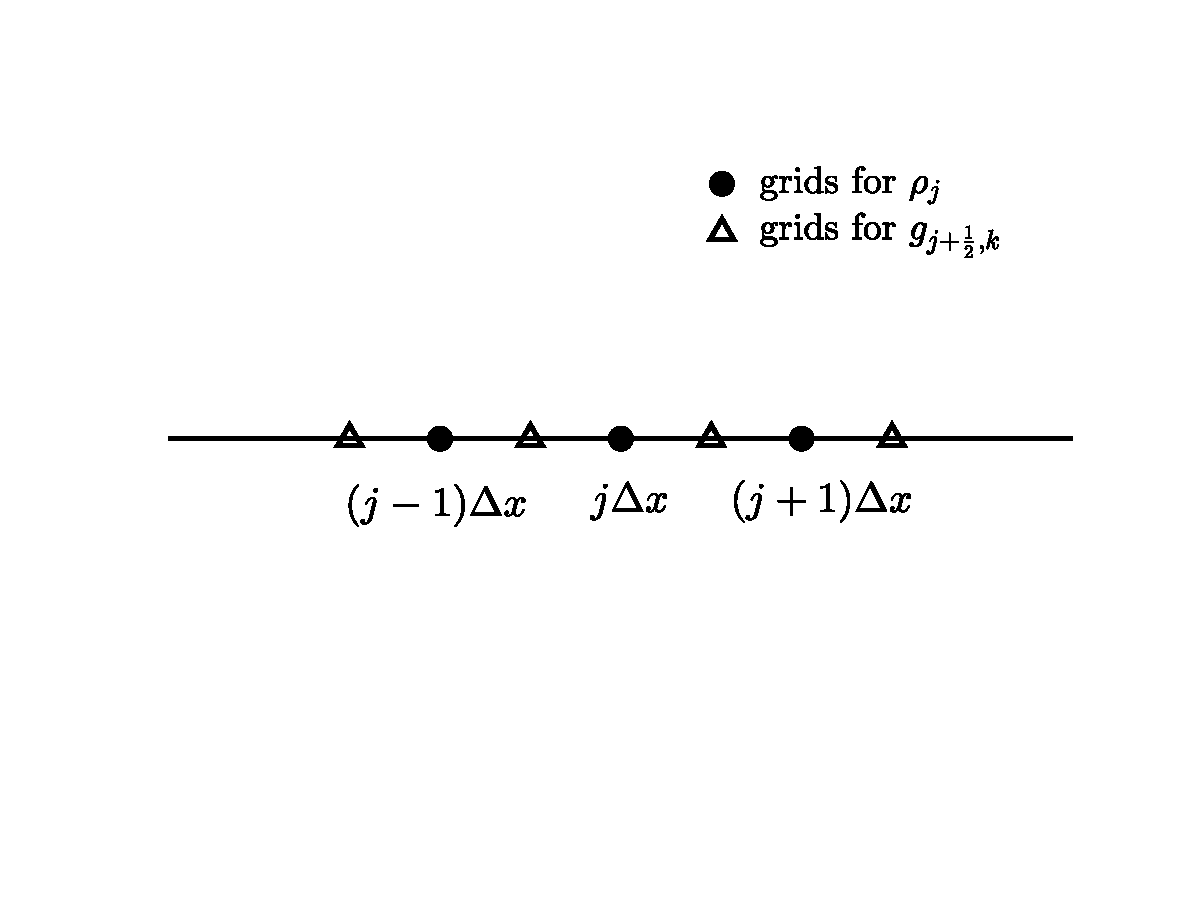
\includegraphics[scale = 0.3]{grid_illustration_1D.eps}
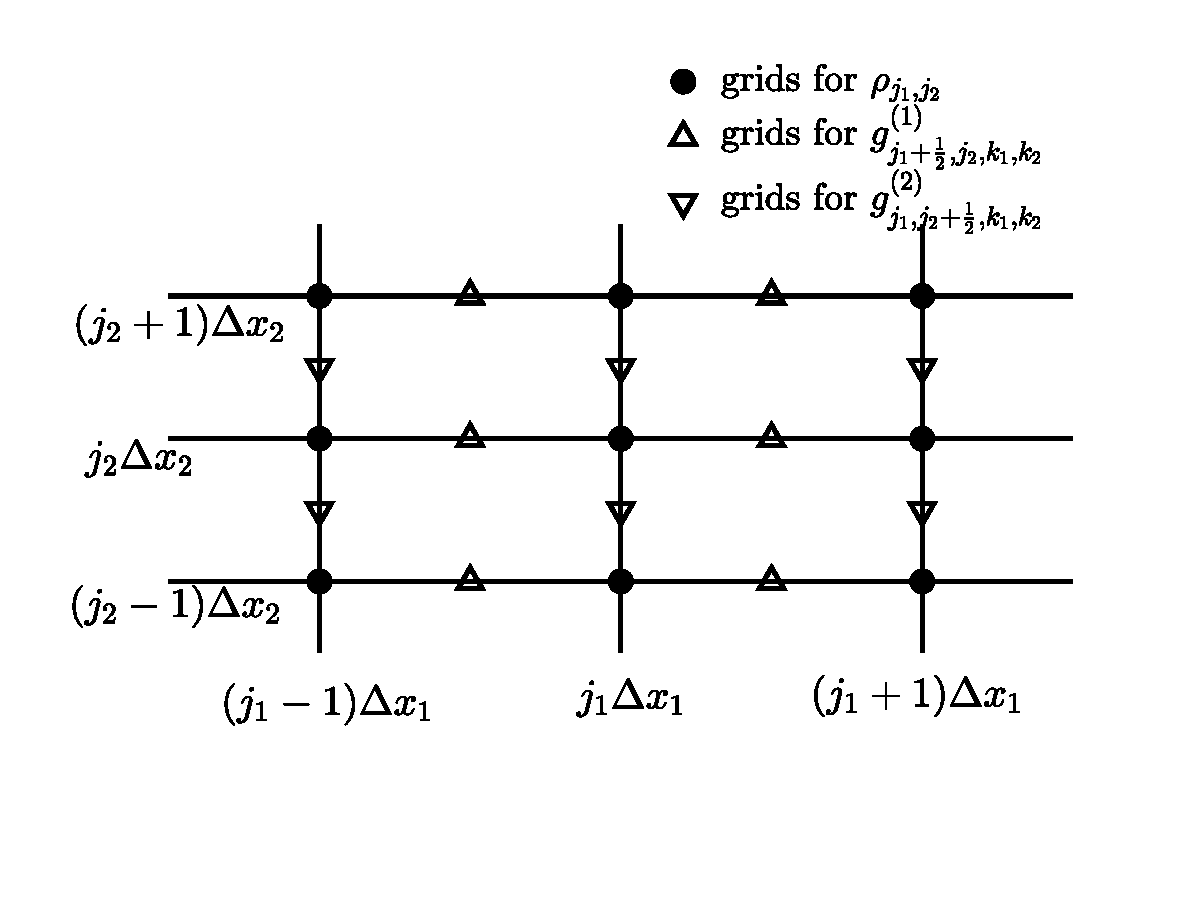
\includegraphics[scale = 0.3]{grid_illustration_2D.eps}
}
\caption{Illustration of the grids in $\mathbf{x}$-space for computing $\rho(t,\mathbf{x})$ and $g(t,\mathbf{x},\mathbf{v})$ in 1D and 2D.}
\label{fig:grid_illstration}
\end{figure}

With the notations defined, the 2D kinetic model \eqref{eq:kinetic_approx} can be discretized as 
\begin{align}
\label{eq:scheme_2D}
    \begin{cases}
    & \delta_t^+ \rho_{j_1,j_2}^n +  
    \sum_{k_1,k_2} \left[v_{k_1}\delta_{x_1}(q( {\bar{\rho}}_{*,j_2}^n) g_{*,j_2,k_1,k_2}^{(1), n+1})_{j_1} +  v_{k_2}\delta_{x_2}(q( {\bar{\rho}}_{j_1,*}^n) g_{j_1,*,k_1,k_2}^{(2), n+1})_{j_2}\right]\Delta v_1 \Delta v_2\\
     & \quad + D_h \left[ \delta_{x_1}( {\bar{\rho}}_{*,j_2}^n q'( {\bar{\rho}}_{*,j_2}^n)\delta_{x_1} \rho_{*,j_2}^{n+1})_{j_1} + \delta_{x_2}( {\bar{\rho}}_{j_1,*}^n q'( {\bar{\rho}}_{j_1,*}^n)\delta_{x_2} \rho_{j_1,*}^{n+1})_{j_2} \right]
    = r_0 \rho_{j_1,j_2}^{n}\left(1 - \frac{\rho_{j_1,j_2}^n}{\rho_{\rm max}}\right)_+,\\
    &\delta_t^+ g_{j_1+\frac12,j_2,k_1, k_2}^{(1),n} + \frac{1}{\varepsilon}(I-\Pi_h) K_{j_1+\frac12,j_2,k_1, k_2}^{(1),n} \\
    &\qquad = \frac{1}{\varepsilon^2}(S_{j_1+\frac12,j_2,k_1,k_2}^{(1), n, n+1} - q( {\bar{\rho}}_{j_1+\frac12,j_2}^n) g_{j_1+\frac12,j_2,k_1,k_2}^{(1), n+1}) + r_0 g_{j_1+\frac12,j_2,k_1,k_2}^{(1),n}\left(1 - \frac{\rho_{j_1+\frac12,j_2}^n}{\rho_{\rm max}}\right)_+,\\
        &\delta_t^+ g_{j_1,j_2+\frac12,k_1, k_2}^{(2),n} + \frac{1}{\varepsilon}(I-\Pi_h) K_{j_1,j_2+\frac12,k_1, k_2}^{(2),n} \\
    & \qquad = \frac{1}{\varepsilon^2}(S_{j_1,j_2+\frac12,k_1,k_2}^{(2), n, n+1} - q( {\bar{\rho}}_{j_1,j_2+\frac12}^n) g_{j_1,j_2+\frac12,k_1,k_2}^{(2), n+1}) + r_0 g_{j_1,j_2+\frac12,k_1,k_2}^{(2),n}\left(1 - \frac{\rho_{j_1,j_2+\frac12}^n}{\rho_{\rm max}}\right)_+,\\
    & (\delta_{x_1}^2 + \delta_{x_2}^2) c_{j_1,j_2}^{n+1} + \rho_{j_1,j_2}^{n+1} - c_{j_1,j_2}^{n+1} = 0,
\end{cases}
\end{align}
where 
{ 
$D_h=\sum_{k_1,k_2} v_{k_i}^2 \psi_{0}(v_{k_1},v_{k_2})\Delta v_1 \Delta v_2$, $i=1$ or 2, and  
}
$\Pi_h$ is the discrete projection operator defined as 
\begin{equation*}
    \Pi_h \eta_{j_1,j_2,k_1,k_2}^n = \sum_{k_1,k_2}\eta_{j_1,j_2,k_1,k_2}^n \psi_{0}(v_{k_1},v_{k_2})\Delta v_1 \Delta v_2
\end{equation*} 
for some general function $\eta(t,\mathbf{x},\mathbf{v})$ and 
\begin{align*}
    & K_{j_1+\frac12,j_2,k_1, k_2}^{(1),n}  = v_{k_1}^+\delta_{x_1}(q( {\bar{\rho}}_{*,j_2}^n) g_{*,j_2,k_1,k_2}^{(1),n})_{j_1} - v_{k_1}^-\delta_{x_1}(q( {\bar{\rho}}_{*,j_2}^n) g_{*,j_2,k_1,k_2}^{(1),n})_{j_1+1}\\
    & \qquad + v_{k_2}^+\delta_{x_2}(q( {\bar{\rho}}_{j_1+\frac12,*}^n) g_{j_1+\frac12, *,k_1,k_2}^{(1),n})_{j_2-\frac12} - v_{k_2}^-\delta_{x_2}(q( {\bar{\rho}}_{j_1+\frac12,*}^n) g_{j_1+\frac12,*,k_1,k_2}^{(1),n})_{j_2+\frac12} \\
    &\qquad + \psi_{0}(v_{k_1}, v_{k_2})\delta_{x_1}\left\{ {\rho}_{*,j_2}^n q'( {\rho}_{*,j_2}^n)\left[v_{k_1}^2\delta_{x_1}\bar{\rho}_{*,j_2}^n + v_{k_1}v_{k_2}(\delta_{x_2}\bar{\rho}_{*,**}^n)_{j_2} \right]\right\}_{j_1+\frac12}\ , \\
    &\qquad + \psi_{0}(v_{k_1}, v_{k_2})\delta_{x_2}\left\{ {\bar{\rho}}_{j_1+\frac12,*}^n q'( {\bar{\rho}}_{j_1+\frac12,*}^n)\left[v_{k_1}v_{k_2}(\delta_{x_1}\bar{\rho}_{**,*}^n)_{j_1+\frac12} + v_{k_2}^2 \delta_{x_2}\bar{\rho}_{j_1+\frac12,*}^n\right]\right\}_{j_2}\ , \\
    & K_{j_1,j_2+\frac12,k_1, k_2}^{(2),n}  = v_{k_1}^+\delta_{x_1}(q( {\bar{\rho}}_{*,j_2+\frac12}^n) g_{*,j_2+\frac12,k_1,k_2}^{(1),n})_{j_1-\frac12} - v_{k_1}^-\delta_{x_1}(q( {\bar{\rho}}_{*,j_2+\frac12}^n) g_{*,j_2+\frac12,k_1,k_2}^{(1),n})_{j_1+\frac12}\\
    & \qquad + v_{k_2}^+\delta_{x_2}(q( {\bar{\rho}}_{j_1,*}^n) g_{j_1, *,k_1,k_2}^{(1),n})_{j_2} - v_{k_2}^-\delta_{x_2}(q( {\bar{\rho}}_{j_1,*}^n) g_{j_1,*,k_1,k_2}^{(1),n})_{j_2+1} \\
    &\qquad + \psi_{0}(v_{k_1}, v_{k_2})\delta_{x_1}\left\{ {\bar{\rho}}_{*,j_2+\frac12}^n q'( {\bar{\rho}}_{*,j_2+\frac12}^n)\left[v_{k_1}^2\delta_{x_1}\bar{\rho}_{*,j_2+\frac12}^n + v_{k_1}v_{k_2}(\delta_{x_2}\bar{\rho}_{*,**}^n)_{j_2+\frac12} \right]\right\}_{j_1}\ , \\
    &\qquad + \psi_{0}(v_{k_1}, v_{k_2})\delta_{x_2}\left\{ {\rho}_{j_1,*}^n q'( {\rho}_{j_1,*}^n)\left[v_{k_1}v_{k_2}(\delta_{x_1}\bar{\rho}_{**,*}^n)_{j_1} + v_{k_2}^2 \delta_{x_2}\bar{\rho}_{j_1,*}^n \right]\right\}_{j_2+\frac12}\ , \\
    & S_{j_1+\frac12, j_2, k_1, k_2}^{(1), n, n+1} = -\psi_{0}(v_{k_1}, v_{k_2})q( \bar{{\rho}}_{j_1+\frac12,j_2}^n)  \left[v_{k_1} \delta_{x_1} \rho_{j_1+\frac12, j_2}^{n+1} + v_{k_2} \delta_{x_2} \bar{\rho}_{j_1+\frac12, j_2}^{n+1} \right] \\
    & \qquad  + \phi_{1}(v_{k_1}, v_{k_2})\delta_{x_1} c_{j_1+\frac12,j_2}^n \Phi^{(1),n+1,n}_{j_1+\frac12,j_2}+\phi_{2}(v_{k_1}, v_{k_2}) \delta_{x_2} c_{j_1+\frac12,j_2}^n
    \Phi^{(2),n+1,n}_{j_1+\frac12,j_2}
    \ ,\\
    & S_{j_1, j_2+\frac12, k_1, k_2}^{(2), n, n+1} = -\psi_{0}(v_{k_1}, v_{k_2})q( \bar{{\rho}}_{j_1,j_2+\frac12}^n)  \left[v_{k_1} \delta_{x_1} \bar{\rho}_{j_1, j_2+\frac12}^{n+1} + v_{k_2} \delta_{x_2} \rho_{j_1, j_2+\frac12}^{n+1} \right] \\
    & \qquad  + \phi_{1}(v_{k_1}, v_{k_2})\delta_{x_1} c_{j_1,j_2+\frac12}^n\Phi^{(1),n+1,n}_{j_1,j_2+\frac12} +\phi_{2}(v_{k_1}, v_{k_2}) \delta_{x_2} c_{j_1,j_2+\frac12}^n 
    \Phi^{(2),n+1,n}_{j_1,j_2+\frac12}
    \ ,
\end{align*}
where, as in the 1D case, both $\Phi^{(1), n_1,n}$ and $\Phi^{(1), n_1,n}$ are upwind approximations of $q(\rho)\rho$ at $t=t_n$ and defined as 
\begin{align*}
    & \Phi^{(1), n_1,n}_{j_1, j_2} = 
	\begin{cases}
		\rho_{j_1 - \frac12,j_2}^{n_1} q(\rho_{j_1+\frac12,j_2}^n)\ , \quad & \text{ if } \delta_{x_1} c_{j_1,j_2}^n \ge 0\ , \\
		\rho_{j_1+\frac12,j_2}^{n_1} q(\rho_{j_1-\frac12,j_2}^n)\ , \quad & \text{ if } \delta_{x_1} c_{j_1,j_2}^n <0\ , 
	\end{cases}\\
	& \Phi^{(2), n_1,n}_{j_1, j_2} = 
	\begin{cases}
		\rho_{j_1,j_2 - \frac12}^{n_1} q(\rho_{j_1,j_2+\frac12}^n)\ , \quad & \text{ if } \delta_{x_2} c_{j_1,j_2}^n \ge 0\ , \\
		\rho_{j_1,j_2+\frac12}^{n_1} q(\rho_{j_1,j_2-\frac12}^n)\ , \quad & \text{ if } \delta_{x_2} c_{j_1,j_2}^n <0\ ,
	\end{cases}
\end{align*}

As for the 1D case, we can formally prove the asymptotic preserving property of the 2D scheme \eqref{eq:scheme_2D} in a similar way. 
In fact, when $\varepsilon\to 0$, we expect that  
\begin{equation*}
	S_{j_1+\frac12, j_2, k_1, k_2}^{(1), n, n+1} = q( {\bar{\rho}}_{j_1+\frac12,j_2}^n) g_{j_1+\frac12,j_2,k_1,k_2}^{(1), n+1}, \  S_{j_1, j_2+\frac12, k_1, k_2}^{(2), n, n+1} = q( {\bar{\rho}}_{j_1,j_2+\frac12}^n) g_{j_1,j_2+\frac12,k_1,k_2}^{(2), n+1},
\end{equation*}
from where we have
\begin{align*}
  & q( {\bar{\rho}}_{j_1+\frac12,j_2}^n) g_{j_1+\frac12,j_2,k_1,k_2}^{(1), n+1} = -\psi_{0}(v_{k_1}, v_{k_2})q( \bar{\rho}_{j_1+\frac12,j_2}^n)  \left[v_{k_1} \delta_{x_1} \rho_{j_1+\frac12, j_2}^{n+1} + v_{k_2} \delta_{x_2} \bar{\rho}_{j_1+\frac12, j_2}^{n+1} \right] \nonumber \\
        & \qquad  + \phi_{1}(v_{k_1}, v_{k_2})\delta_{x_1} c_{j_1+\frac12,j_2}^n \Phi^{(1),n+1,n}_{j_1+\frac12,j_2}+\phi_{2}(v_{k_1}, v_{k_2}) \delta_{x_2} c_{j_1+\frac12,j_2}^n
        \Phi^{(2),n+1,n}_{j_1+\frac12,j_2},\\
	&q( \bar{\rho}_{j_1,j_2+\frac12}^n) g_{j_1,j_2+\frac12,k_1,k_2}^{(2), n+1} = -\psi_{0}(v_{k_1}, v_{k_2})q( \bar{\rho}_{j_1,j_2+\frac12}^n)  \left[v_{k_1} \delta_{x_1} \bar{\rho}_{j_1, j_2+\frac12}^{n+1} + v_{k_2} \delta_{x_2} \rho_{j_1, j_2+\frac12}^{n+1} \right] \nonumber\\
    & \qquad  + \phi_{1}(v_{k_1}, v_{k_2})\delta_{x_1} c_{j_1,j_2+\frac12}^n\Phi^{(1),n+1,n}_{j_1,j_2+\frac12} +\phi_{2}(v_{k_1}, v_{k_2}) \delta_{x_2} c_{j_1,j_2+\frac12}^n 
    \Phi^{(2),n+1,n}_{j_1,j_2+\frac12}\ .
\end{align*}
Substituting into the first equation in \eqref{eq:scheme_2D} and using the fact that
\begin{align*}
	&\sum_{k_1,k_2} v_{k_i}v_{k_j} \psi_0(v_{k_1},v_{k_2}) \Delta v_1 \Delta v_2 = D_h \delta_{i,j},  
	&\sum_{k_1,k_2} v_{k_i} \phi_j(v_{k_1},v_{k_2}) \Delta v_1 \Delta v_2 = \chi_0\delta_{i,j},                   
\end{align*}
for $i,j = 1,2$, 
we recover the finite difference scheme for the macro model 
\begin{align*}
	&\delta_t^+ \rho_{j_1,j_2}^n   
    	- D_h \delta_{x_1} \left( d(\bar{\rho}_{*,j_2}^n) \delta_{x_1} \rho_{*,j_2}^{n+1}\right)_{j_1} 
	- D_h \delta_{x_2} \left( d(\bar{\rho}_{j_1,*}^n)\delta_{x_2} \rho_{j_1, *}^{n+1} \right)_{j_2} 	\nonumber \\
	 & \quad + \chi_0\delta_{x_1}\left[\Phi_{*,j_2}^{(1),n+1,n}\delta_{x_1} c_{*,j_2}^n\right]_{j_1} 
	 + \chi_0\delta_{x_2}\left[\Phi_{j_1,*}^{(1),n+1,n}\delta_{x_2} c_{j_1,*}^n\right]_{j_2}
    = r_0 \rho_{j_1,j_2}^{n}\left(1 - \frac{\rho_{j_1,j_2}^n}{\rho_{\rm max}}\right)_+\ ,
\end{align*}
where $d(\rho_{j_1,j_2}^n) = q(\rho_{j_1,j_2}^n) - \rho_{j_1,j_2}^n q'( \rho_{j_1,j_2}^n)$.

\section*{Acknowledgments}
The authors wish to thank L. Almeida and K. J. Painter for helpful discussions and guidance.

\section*{Fundings}
This work was supported by Sorbonne Alliance University with an Emergence project MATHREGEN, grant number S29-05Z101, by Agence Nationale de la Recherche (ANR) under the project grant number ANR-22-CE45-0024-01, the Fondation Sciences Mathématiques de Paris (FSMP), the Advanced Grant Nonlocal-CPD (Nonlocal PDEs for Complex Particle Dynamics: Phase Transitions, Patterns and Synchronization) of the European Research Council Executive Agency (ERC), the project MoGlimaging, Plan Cancer THE Call, from INSERM, France, 
the R\&D Program of Beijing Municipal Education Commission from China, grant number KM202310028016, 
and the National Natural Science Foundation of China, grant number 12201436.

\bibliographystyle{siamplain}
\bibliography{AP_method}
\end{document}
